\chapter{Einleitung}

\begin{fquote}[Mark Zuckerberg][Facebook CEO][2014]
Virtual reality was once the dream of science fiction. But the internet was also once a dream, and so were computers and smartphones. The future is coming.
\end{fquote}

\begin{fquote}[Tim Cook][Apple CEO][2017]
I think AR is [...] big, it’s huge. I get excited because of the things that could be done that could improve a lot of lives.
\end{fquote}

\section{Einführung in die AR}
Viele der einflussreichsten Technologieunternehmen arbeiten an der \emph{Virtual} bzw.\ \emph{Augmented Reality (VR} bzw.\ \emph{AR)}. Tim Cook ist überzeugt davon, dass die AR die nächste \emph{``big idea''} nach dem Smartphone wird \cite{theindependent2017apple}.

Nicht nur Großkonzerne wie Apple, Facebook oder Samsung arbeiten intensiv in diesem Bereich. Ein Start-up-Unternehmen namens \emph{Magic Leap} entwickelt eine AR Brille und wird von Investoren in Billionenhöhe unterstützt \cite{kelly2016untold}. Laut einem Cover-Artikel der Zeitschrift \emph{Wire} ist die noch unter Verschluss gehaltene Technologie den Konkurrenzprodukten allen voraus. Das Release der Hardware ist Stand heute noch nicht bekannt, aber es lässt sich ein Trend erkennen, der die nächsten Jahre viele neue Möglichkeiten eröffnen wird und möglicherweise die Digitalisierung revolutionieren wird.
Diese Arbeit wird sich mit einer Anwendung der AR beschäftigen -- der Softwarevisualisierung. Die Spezialisierung auf AR kann nach der Abgrenzung von AR und VR besser nachvollzogen werden.

\paragraph{VR} ist eine Umgebung, in der der Betrachter vollkommen von einer computergenerierten Welt umgeben ist, die oft die reale Welt imitiert, aber auch rein fiktiv sein kann \cite{milgram1995augmented}.\\

Obwohl der Begriff AR zunehmend in der Industrie Verwendung findet, entbehrt er doch einer einheitlichen Definition. In \cite{azuma1997survey} wird AR als \emph{"`Variation"'} von VR betrachtet. Dagegen vermittelt P.\ Milgrim in \cite{milgram1995augmented} ein vollständigeres Verständnis, weshalb sich die Begrifflichkeiten in dieser Arbeit daran anlehnen sollen. Nach Milgrim existieren die beiden entgegengesetzten Extreme der Realität und der Virtualität. Alles dazwischen ist die sogenannte \emph{Mixed Reality (MR)}.

\paragraph{MR} ist eine Umgebung, in der Elemente der realen und einer virtuellen Welt zusammen dargestellt werden \cite{kato1999marker}.\\

\begin{figure}[htb]
  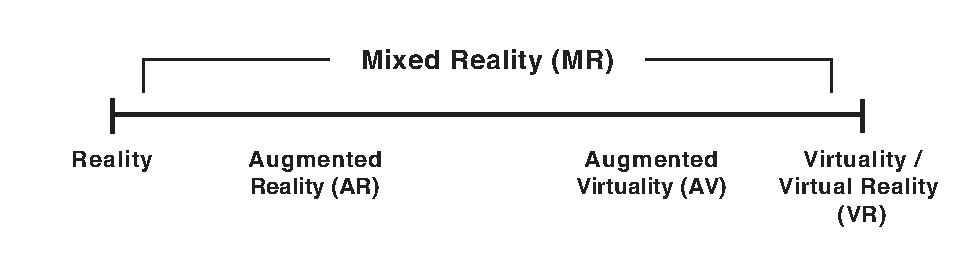
\includegraphics[width=.8\textwidth]{\figdir/rv-continuum}
  \caption{Das Reality-Virtuality-Kontinuum (nach \cite{milgram1995augmented})}
  \label{fig:rv-continuum}
\end{figure}

Dieses \emph{Reality-Virtuality-Kontinuum} ist in Abbildung \ref{fig:rv-continuum} dargestellt, in dem gut zu erkennen ist, dass AR zu der Mixed Reality gehört. In den meisten Quellen wie \cite{azuma1997survey, azuma2001recent, kato1999marker} wird bei der AR noch die Komponente der Interaktion aufgeführt. AR kann deshalb folgendermaßen definiert werden:

\begin{defbox}{AR}{ar}
   AR ist die Erweiterung der realen Welt durch computergenerierte Elemente, mit denen der Betrachter in Echtzeit interagieren kann.
\end{defbox}

Auch die \emph{Augmented Virtuality}, also die Erweiterung der virtuellen Welt durch reale Elemente, gehört zur MR.

Wie viele der einflussreichsten Menschen der Technologie-Industrie, sieht Tim Cook mehr Zukunft in der AR. Er begründet das in einem Interview damit, dass diese Technologie die wirkliche Welt nicht ausschließt, sondern die Realität erweitert und Teil von zwischenmenschlicher Kommunikation sein kann \cite{theindependent2017apple}.

Wir stellen uns ein Hologramm vor, dass auf einem Konferenztisch Gestalt annimmt und eine Software visualisiert. Entwickler, Projektleiter oder auch Kunden versammeln sich um den Tisch und können miteinander interaktiv die Software betrachten, evaluieren und wichtige Informationen daraus ziehen.

Dies wäre mit VR nicht möglich, da der Betrachter von der Außenwelt abgeschottet ist. Deshalb wird im Zuge dieser Arbeit mit der Stand heute am weitesten ausgereiften Technologie der AR gearbeitet -- der \emph{HoloLens} von Microsoft.

\section{Motivation für eine Softwarevisualisierung in der AR}
Die Technologie der AR bietet uns viele neue Möglichkeiten. Eine Motivation dieser Arbeit ist es sich produktiv mit einer neuen, zukunftsträchtigen Technologie zu beschäftigen. Das ist jedoch nur die eine Seite. Die weitaus größere Motivation ist, die zuvor noch nicht dagewesene Zugänglichkeit und Interaktion mit dreidimensionaler \emph{Visualisierung} auszunutzen. Visualisierung im Allgemeinen begegnet uns in vielen Bereichen unseres Lebens und nimmt eine wichtige Rolle ein.

Niemand konnte bislang unser Sonnensystem von außen betrachten. Dennoch haben wir alle eine ziemlich gute Vorstellung wie dieses aufgebaut ist. Durch die Visualisierung der Planeten und der Sonne entsteht in uns ein geistiges Abbild der Realität. Das Konzept komplexe Realitäten zu abstrahieren und zu visualisieren, um dadurch die Realität besser verstehen zu können, ist in vielen Disziplinen der Wissenschaft vertreten.

Neben Wissenschaften wie Physik, Chemie oder Biologie, nimmt Visualisierung auch besonders in der Informatik eine wichtige Rolle ein. In vielen Bereichen müssen Informationen in eine visuelle Form gebracht werden, die für das menschliche Auge besser zu lesen sind.

Gerade bei komplexen Software-Systemen ist das der Fall. Soll zum Beispiel die zu Grunde liegende Struktur einer Software Außenstehenden erklärt werden, gelingt das mit einem visuellen Modell wie einem UML-Diagramm sicherlich besser, als nur in den Source-Code zu schauen.

So wie UML-Diagramme, war die Darstellungsform der Softwarevisualisierung bislang meist zweidimensional. Mit AR wird dieser Disziplin der Visualisierung jedoch wortwörtlich ein neuer Raum an Möglichkeiten eröffnet und diese Arbeit soll damit beginnen den Raum ausfüllen.

\section{Zielsetzung der Arbeit}
Für die Zielsetzung einer 3D Softwarevisualisierung in der AR sollten zunächst die allgemeinen Ziele einer Softwarevisualisierung betrachtet werden. Softwarevisualisierung ist für Diehl die "`visualization of artifacts related to software and its development process"' \cite{diehl2007software}. Diese Definition ist sehr breit gefasst. Wird der Fokus mehr auf die Nutzerorientierung gelegt, lässt sich Softwarevisualisierung wie folgt definieren:

\begin{defbox}{Softwarevisualisierung}{software-visualization}
Softwarevisualisierung ist die bildliche oder auch metaphorische Darstellung einer Software, um dem Nutzer durch Vereinfachung und Abstraktion das bessere Verständnis oder die einfachere Analyse von Software zu ermöglichen.
\end{defbox}

In dieser Arbeit soll eine solche Softwarevisualisierung für die AR vorgestellt werden. Das neuartige Konzept \emph{CodeLeaves} bedient sich der Metapher des \textit{Software-Waldes} und soll vorgestellt und im Detail ausgearbeitet werden.

Im Vorfeld dieser Arbeit wurde in einer Studie erkannt, dass eine gute Softwarevisualisierung sowohl statische als auch dynamische Daten unterstützen sollte. Mit CodeLeaves soll dies möglich sein. Beliebige Daten sollen übersichtlich auf die Struktur der Software abgebildeten werden können.

Durch Expertengespräche sollen User-Storys erstellt werden, um den Mehrwert des neuen Konzepts zu veranschaulichen und für weitere Überlegungen Anforderungen zu definieren.

Um den Anforderungen gerecht zu werden, soll für CodeLeaves ein sprachunabhängiges Datenmodell entworfen werden, dass alle geforderten Informationen unterstützt.

Der Praktische Teil dieser Arbeit soll die prototypische Entwicklung von CodeLeaves sein. Dabei sollen zwei Schwerpunkte gesetzt werden. Zum einen soll die Generierung des Waldes und die dafür benötigten Layout-Algorithmen erarbeitet und für die HoloLens umgesetzt werden. Zum anderen soll ein Interkations-Konzept ausgearbeitet werden, mit dem CodeLeaves bedienbar wird und eine Software bis ins Detail erforscht werden kann.

\section{Aufbau der Arbeit}
Im nächsten Kapitel wird das Konzept von CodeLeaves zunächst auf High-Level-Ebene vorgestellt, um es anschließend detaillierter zu erörtern. Es werden Begriffe definiert, die für weitere Inhalte ein einheitliches Verständnis schaffen. Nachdem das Konzept verstanden wurde, werden Unterschiede und Vorteile von CodeLeaves zu alternativen 3D Softwarevisualisierungen hervorgehoben. Die Befragung von Experten der Softwareanalyse und die daraus abgeleiteten Anforderungen an CodeLeaves \ref{sec:requirements} schließen das erste Kapitel ab.

Das Kapitel \ref{ch:data-model} beschäftigt sich mit der Entwicklung eines geeigneten Datenmodells für CodeLeaves. Nachdem vorhandene Datenmodelle auf Tauglichkeit für CodeLeaves überprüft wurden, wird ein neues, in Schichten getrenntes Datenmodell entwickelt.

Mit diesem Datenmodell kann der Wald für CodeLeaves generiert werden, was Thema des \ref{ch:layout}. Kapitels ist. In diesem Zuge werden zwei Algorithmen und die verwendete Mathematik vorgestellt, die eine möglichst natürliche und übersichtliche Struktur des Waldes produzieren. Abbildungen der HoloLens-Applikation zeigen die praktische Anwendung der theoretischen Inhalte.

Kapitel \ref{ch:interaction-ar} behandelt Grundlagen der Interaktion in der AR, die bei der Interaktion mit CodeLeaves Anwendung finden. Es wird auch beschrieben wie mit reaktiver Programmierung die Interaktion technisch sinnvoll umgesetzt werden kann.

Die Interaktion mit CodeLeaves ist Thema des Kapitels \ref{ch:interaction}. Es wird gezeigt wie CodeLeaves mit den zur Verfügung stehenden Eingabemöglichkeiten bis ins Detail exploriert werden kann.

Das Kapitel \ref{ch:conclusion} fasst die Ergebnisse der Arbeit zusammen und ein Ausblick auf weiterführende Arbeiten runden die Arbeit ab.

\section{Abgrenzung}
\label{sec:distinction}

Die Beschaffung der Informationen über eine Software wird hier nur am Rande betrachtet. Für die Analyse einer Software müssen statische und dynamische Informationen gesammelt und aggregiert werden. Dafür gibt es verschiedenste Tools Open-Source- und proprietäre Tools. Die Anbindung an CodeLeaves würde den Rahmen dieser Arbeit jedoch bei Weitem sprengen. Diese Arbeit stellt jedoch den Anspruch, dass mit realistischen Beispieldaten gearbeitet wird, um eine valide Einschätzung des Mehrwerts von CodeLeaves geben zu können.

Weiterhin wird im Zuge dieser Arbeit mit Prototypen gearbeitet. Diese sind kein fertiges Produkt der Softwarevisualisierung, sondern dienen vielmehr einen technischen Durchstich für die HoloLens und als Basis für eine weiterführende Entwicklung.

\chapter{Das Konzept CodeLeaves}
\label{ch:concept}

\section{CodeLeaves und die Metapher Software-Wald}
\label{sec:idea}

\emph{``Hierarchies are almost ubiquitous [...]''} \cite{robertson1991cone} halten Robertson \emph{et al.}
 schon 1991 bei der Visualisierung von hierarchischen Informationen fest. So verhält es sich auch bei der Struktur einer Software. Jede Software mit einer geschachtelten Struktur ist hierarchisch und kann mithilfe eines Baumes dargestellt werden. \emph{"`Bäume sind eine der wichtigsten Datenstrukturen, die besonders im Zusammenhang mit hierarchischen Abhängigkeiten und Beziehungen zwischen Daten von Vorteil sind."'} \cite{ernst2016grundkurs} stellen auch Ernst \emph{et al.} fest.

Der Baum in der Informatik zeugt von einer ursprünglichen Metapher -- dem Baum, wie er draußen in der Natur wächst. Da dieser unbestritten dreidimensional ist, liegt eine Softwarevisualisierung für die Dreidimensionalität mit einer realitätsnahen Interpretation der Baum-Metapher nicht fern. Werden Bäume in 3D in natürlicher Wuchsrichtung modelliert und mehrere Bäume für eine Software verwendet, entsteht eine neue Metapher: der \emph{Software-Wald}.

CodeLeaves stellt ein Konzept dar, dass sich die Metapher des Software-Waldes zu nutze macht und wird im Folgenden auf High-Level-Ebene skizziert und danach genauer erläutert:

\begin{titlebox}{\textbf{Konzept:} CodeLeaves}
  \begin{enumerate}[leftmargin=1em]
    \item Die Struktur der Software wird mit nach oben wachsenden Bäumen dargestellt.
    \item Pakete\ im Hauptverzeichnis werden als Bäume, Unterpakete als Äste und Klassen als Blätter dargestellt.
    \item Die Blätter der Bäume können durch ihre Farbe eine beliebige \textit{Metrik}\footnotemark[1]{} visualisieren.
    \item \textit{Verbindungen}\footnotemark[2]{} zwischen einzelnen Klassen werden aggregiert auf die Struktur der Bäume als Dicke der Kanten abgebildet oder interaktiv als direkte \emph{Spinnweben} dargestellt.
    \item Zwischen den Bäumen entsteht ein Geflecht aus \emph{Wurzeln}, was aggregierte Verbindungen zwischen den Bäumen darstellt.
  \end{enumerate}
\end{titlebox}

%\footnotetext{siehe Definition \ref{def:softwareartefact}}
\stepcounter{footnote}
\footnotetext{siehe Definition \ref{def:metric}}
\stepcounter{footnote}
\footnotetext{siehe Definition \ref{def:connection}}

\paragraph{Punkt 1} ist dafür verantwortlich, dass der geistige Transfer zwischen realer Software und deren Visualisierung möglichst gering ist. Das bedeutet auch, dass diejenigen, die tatsächlich mit der Software arbeiten, sich aufgrund der bekannten Baumstruktur auch in der Visualisierung schnell zurecht finden. Im Fachjargon wird hier von der \emph{Habitability} gesprochen, also wie schnell oder gut sich ein Betrachter in einer Software oder auch deren Visualisierung "`zuhause"' fühlt \cite{wettel2007program}.

\paragraph{Punkt 2} beschreibt die Überführung der Struktur einer Software in einen Wald. Dabei sollen Klassen im Weiteren beispielhaft als die kleinsten betrachteten \textit{Softwareartefakte} angesehen werden.

\begin{defbox}{Softwareartefakt}{softwareartefact}
  Ein Softwareartefakt ist eine definierte Einheit einer Software.
\end{defbox}

Bei feinerer Granularität könnten Klassen aber auch mit Methoden oder sogar Code-Blöcke ersetzt werden. Für Softwareartefakte, die aus anderen Softwareartefakten bestehen, einigen wir uns auf die Bezeichnung Paket. Auch hier gilt, dass die Organisation von Software genauso in Module oder Komponenten aufgebaut sein kann, solange sie hierarchisch ist.
 
Die Darstellung einzelner Bäume für die Pakete im Hauptverzeichnis einer Software bietet sich an. Dieser Ansatz schließt jedoch nicht aus, dass Pakete aus einer tieferen Hierarchie-Ebene als neuer Waldboden verwendet werden. Interaktionen dieser Art sind Teil des Kapitels \ref{ch:interaction}. 

\paragraph{Punkt 3} bedeutet, dass in CodeLeaves durch die Farbe der Blätter eine gute Übersicht über eine ausgewählte Metrik der Software entsteht.

\begin{defbox}{Metrik}{metric}
  Eine Metrik ist eine Eigenschaft, die für jede Klasse gemessen und mit einem eindeutigen Zahlenwert festgelegt werden kann. Ein Beispiel dafür ist die Testabdeckung von Klassen.
\end{defbox}

Beispielsweise kann der Farbe der Blätter die Testabdeckung der einzelnen Klassen zugewiesen werden. Mit einer Skala von Grün bis Rot kann dann der Software-Wald bei guter Testabdeckung im sommerlichen Grün erstrahlen, oder bei einer weniger guten Testabdeckung eher in den Herbst übergehen. Die Färbung der Blätter ist flexibel auf jegliche Metrik anwendbar, die für die betrachtete Software zur Verfügung steht.

\paragraph{Punkt 4} heißt, dass die Verbindungen einer Software sehr übersichtlich auf die Struktur der Software abgebildet werden können, ohne diese negativ zu beeinflussen. Eine Verbindung in einer Software und die Aggregation einer solchen wird im Folgenden für das bessere Verständnis definiert.

\begin{defboxfullwidth}{Verbindung}{connection}
Unter einer Verbindung in einer Software verstehen wir eine gerichtete Beziehung eines bestimmten Typs zwischen zwei Klassen. Eine Klasse kann mehrere ein- und ausgehende Verbindungen besitzen. Ein Beispiel für ein Verbindungs-Typ sind statische Abhängigkeiten von Klassen.
\end{defboxfullwidth}



\begin{splitbox}{Aggregation von Verbindungen}{aggregation}
Bei der Aggregation von Verbindungen zwischen Klassen werden die Verbindungen nicht direkt dargestellt, sondern über die Eltern geleitet. Seien $x, y$ Pakete und Klasse $A \in x$ besitze eine Verbindung zu Klasse $B \in y$, dann geht die Verbindung von $A$ zunächst zu $x$. Angenommen $x$ und $y$ befinden sich zudem im Paket $z$, dann geht die aggregierte Verbindung weiter über $z$ zu $y$ und schließlich zu $B$.
\tcblower
%\raggedright
%Beispiel in CodeLeaves:\par\vspace{.6cm}
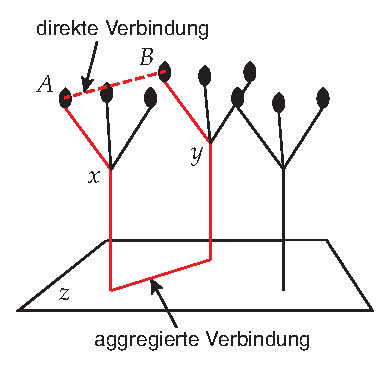
\includegraphics[width=\linewidth]{figures/aggregation}
\end{splitbox}

Auf der rechten Seite der Definition \ref{def:aggregation} ist eine aggregierte Verbindung am Beispiel von CodeLeaves zu sehen.

Bei mehreren Verbindungen zwischen benachbarten Paketen, überlagern sich die aggregierten Abhängigkeiten zwangsläufig. Falls im Beispiel von \ref{def:aggregation} eine weitere Abhängigkeit von einer anderen Klasse in $x$ zu einer anderen Klasse in $y$ bestünde, würden sich die aggregierten Verbindungen von $x$ bis $y$ überlagern. Daraus resultiert, dass nicht jede aggregierte Verbindung ohne Interaktion zwangsläufig eindeutig zuzuordnen ist.

Wird aber bei jedem Verbindungsstück, sei es eine Kante oder Wurzel, die Anzahl an überlagernden Verbindungen als Dicke des Verbindungsstücks dargestellt, bekommt der Betrachter eine gute Übersicht über die Gesamtheit der Verbindungen. Durch Interaktion mit einzelnen Verbindungsstücken soll eine fein granulärere Analyse der Verbindungen möglich sein.

Das zweite Element von Punkt 4 sind Spinnweben. Damit lassen sich die Verbindungen direkt darstellen. Um bei großen Software-Systemen aber die Übersicht über den Wald nicht zu verlieren, sollten diese mithilfe von Interaktion flexibel aktivierbar sein.

\paragraph{Punkt 5} bietet einen goßen Vorteil gegenüber der Zweidimensionalität. In Abbildung \ref{fig:3d-advantage} wird rechts das Prinzip des Wurzelgeflechts mit einem minimalistischen Beispiel illustriert.

\begin{figure}[htb]
  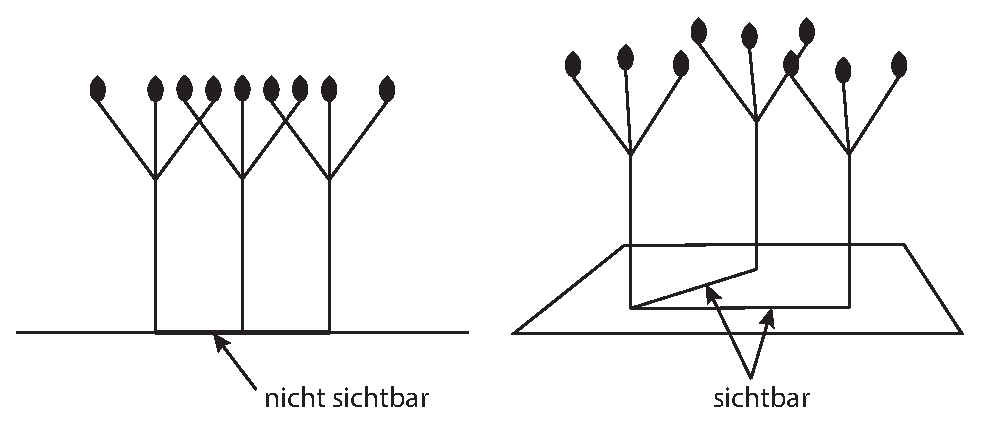
\includegraphics[width=.8\textwidth]{figures/3d-advantage}
  \caption{Vorteil der Dreidimensionalität bei der Darstellung von Wurzeln}
  \label{fig:3d-advantage}
\end{figure}

In 3D sind die Verbindungen zwischen den Bäumen auf einen Blick ersichtlich. Bei Betrachtung der Bäume in 2D, wie es im linken Teil der Abbildung dargestellt ist, verschwinden die Verbindungen hintereinander und sind nicht zuzuordnen.\\

Nachdem das grundlegende Konzept von CodeLeaves verstanden ist, muss eine Begriffsklärung ein einheitliches Verständnis der verwendeten Elemente schaffen. Es wurden bereits Elemente des Waldes intuitiv verwendet, müssen aber für die Verwendung im Datenmodell im nächsten Kapitel sowie in den entwickelten Layout-Algorithmen in Kapitel \ref{ch:layout} genau definiert werden.

\section{Begriffsklärung}
\label{sec:naming}

Die Bezeichnungen, die im Folgenden definiert werden, bauen stark auf die Datenstruktur eines Baumes in der Informatik auf -- \textit{"`the most important nonlinear structures that arise in computer algorithms"'}\cite{knuth1973fundamental} -- die in einschlägiger Literatur wie \cite{knuth1973fundamental, ernst2016grundkurs, gumm2009einfuehrung} definiert wird.

Da sich aber nicht alle Begriffe der Datenstruktur auf die Elemente von CodeLeaves eins-zu-eins übertragen lassen, passen wir einige Begriffe der Datenstruktur an die Gegebenheiten von CodeLeaves an und führen neue Begriffe ein.

\begin{itemize}
  \item Ein \textit{Baum} (engl.: \textit{tree}) besteht aus einer Menge von \textit{Knoten}, die so durch \textit{Kanten} so verbunden sind, dass keine Kreise auftreten (Abgewandelt aus \cite{gumm2009einfuehrung, ernst2016grundkurs}).
  \item Ein \textit{Knoten} beinhaltet Informationen zu sich selbst und hat $0$ bis $n$ \textit{Kinder} (engl.: \textit{childs}).
  \item Ein Knoten mit keinen Kindern wird als \textit{Blatt} (engl.: \textit{leaf}) bezeichnet. Alle anderen Knoten heißen \textit{innere Knoten} (engl.: \textit{inner nodes}) \cite{gumm2009einfuehrung}.
  \item Kinder des selben Knotens werden \textit{Geschwister} (engl.: \textit{siblings}) genannt.
  \item Alle Kinder und Kindeskinder eines Knoten werden \textit{Nachfahren} (engl.: \textit{descendants}) des Knotens genannt.
\end{itemize}

Bei der klassischen Definition eines Baumes wird bei dem Knoten ohne Elternteil von der "`Wurzel"' gesprochen. Im Modell von CodeLeaves ist der unterste Knoten eines Baumes jedoch noch durch eine Kante mit dem Waldboden verbunden. Darüber hinaus überschneidet sich die Bezeichnung von "`Wurzel"' mit den Verbindungen zwischen den einzelnen Bäumen, die bei der klassischen Definition nicht existieren. Deshalb wird für diesen speziellen Knoten eine neue Bezeichnung eingeführt. 

\begin{itemize}
  \item Der unterste Knoten eines Baumes wird als \textit{Kronenansatz} (engl.: \textit{crown base}) bezeichnet.
  \item Alle Knoten bis auf den Kronenansatz haben genau einen Knoten als \textit{Elternteil} (auch Vorfahre genannt, engl.: \textit{parent} oder \textit{ancestor}).
\end{itemize}

Nachdem in den meisten Fällen Bäume in 2D nach unten wachsend dargestellt werden, was wahrscheinlich auf die Tatsache zurück zu führen ist, dass handschriftliche Diagramme tendenziell nach unten wachsend gezeichnet werden \cite{knuth1973fundamental}, wird bei Knoten auch oft von einer Tiefe gesprochen. Diese Bezeichnung wird beibehalten.

\begin{itemize}
  \item Die \textit{Tiefe} eines Knotens gibt an, wie viele Kanten er vom Kronenansatz aus entfernt liegt (Abgewandelt aus \cite{ernst2016grundkurs}).
  \item Die \textit{Höhe} (engl.: \textit{height}) eines Knoten beschreibt die maximale Tiefe aller Nachfahren.
  \item Alle Knoten mit der gleichen Höhe befinden sich auf der selben \textit{Ebene}.
\end{itemize}

Alle nachfolgenden Kanten und Knoten eines Knotens $A$ werden in der Literatur unterschiedlich bezeichnet. Es ist die Rede von "`Teilbaum"' \cite{ernst2016grundkurs} oder auch "`Unterbäumen"' \cite{gumm2009einfuehrung}. Wir definieren dafür einen dem 3D Modell besser entsprechenden Begriff.

\begin{itemize}
  \item Ein \textit{Ast} (engl.: \textit{branch}) ist die Menge aller Nachfahren eines Knotens und die dazugehörigen Kanten.
\end{itemize}

Bisher wurden Bezeichnungen aus Literatur verwendet oder abgeändert. Betrachten wir nun Elemente von CodeLeaves, die so nicht in der klassischen Definition einer Baumes vorkommen.

\begin{itemize}
  \item Der Kronenansatz ist durch die Kante namens \textit{Stamm} (engl.: \textit{trunk}) mit dem \textit{Waldboden} (engl.: forest floor) verbunden.
  \item Der Schnittpunkt zwischen Stamm und Waldboden nennen wir \textit{Stammbasis} (engl.: \textit{trunk base}). Dieser ist jedoch kein Knoten und beinhaltet auch keine Informationen.
  \item Ein Wald mit $n$ Bäumen besitzt $0$ bis $n!$ \textit{Wurzeln} (engl. \textit{roots}), die jeweils zwei Stammbasen miteinander verbinden.
  \item Ein \textit{Wald} besteht aus einer disjunkten Menge an Bäumen, Wurzeln und dem Waldboden.
\end{itemize}

\begin{figure}[htb]
  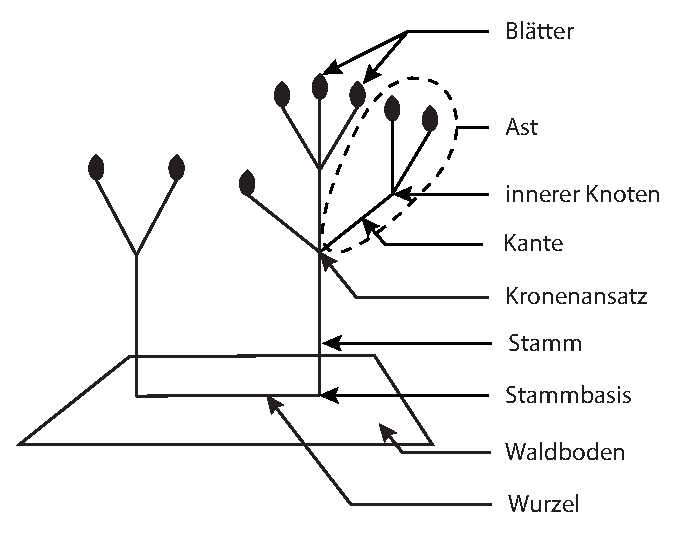
\includegraphics[width=.6\textwidth]{\figdir/naming}
  \caption{Begriffsklärung}
  \label{fig:naming}
\end{figure}

\section{Vergleich mit anderen Konzepten}
\label{sec:comparison}

Im Vorfeld dieser Arbeit wurde in \cite{puetz2017softwarevisualisierung} evaluiert, was eine gute Softwarevisualisierung ausmacht und unterstützen sollte. Ausgehend davon wurden vorhandene und neue Konzepte der 3D Softwarevisualisierungen miteinander verglichen. Die Ergebnisse dieser Untersuchung sollen im Folgenden vorgestellt werden.

Um herauszufinden welchen Mehrwert sich Nutzer einer Softwarevisualisierung von dieser versprechen, wurde eine Umfrage in der QAware GbmH durchgeführt. Die QAware ist ein Projekthaus mit den Kerngeschäften Diagnose, Sanierung, Exploration und Realisierung von Software \cite{qaware2017it-probleme}. Durch die Erfahrung in Projekten für namhafte Kunden zeichnen sich die Mitarbeiter durch fundiertes Wissen und Expertise aus. Es wurden insgesamt 22 Mitarbeiter mit unterschiedlichen Rollen in der Softwareentwicklung befragt.

\begin{figure}[hbt]
\begin{tikzpicture}
  \begin{axis} [
    width = \textwidth,
    height = 8cm,
    symbolic x coords={Lines-of-Code, Testabdeckung, Komplexität, Code-Violations, Struktur, Abhängigkeiten, Anzahl Aufrufe, Ausführungszeiten, Laufzeitfehler, Ressourcen-Auslastung, Evolution der Statik},
    xtick={Lines-of-Code, Testabdeckung, Komplexität, Code-Violations, Struktur, Abhängigkeiten, Anzahl Aufrufe, Ausführungszeiten, Laufzeitfehler, Ressourcen-Auslastung, Evolution der Statik},
    x tick label style={rotate=45, anchor=east, align=center},
    major x tick style = transparent,
    axis lines = left,
    axis line style = {-},
    ymajorgrids = true,
    ylabel=Anzahl,
    ylabel shift =1em,
    legend style = {at={(.99,.98)}, anchor=north east, legend columns=2, column sep=1ex},
    ymin=0,
    bar width=.6cm,
    ybar=-.6cm,
    enlarge x limits={abs=.6cm}
  ]
    \addplot[style={fill=primary}]
      coordinates {(Lines-of-Code, 1) (Testabdeckung, 1) (Komplexität, 3) (Code-Violations, 4) (Struktur, 5) (Abhängigkeiten, 7)};
    \addplot[style={fill=secondary}]
      coordinates {(Anzahl Aufrufe, 5) (Ausführungszeiten, 5) (Laufzeitfehler, 1) (Ressourcen-Auslastung, 1)};
    \addplot[style={fill=tertiary}]
      coordinates {(Evolution der Statik, 4)};

    \legend{Statik, Dynamik, Evolution}

  \end{axis}
\end{tikzpicture}
\caption{Informationen über Software, an deren Visualisierung Mitarbeitern der QAware Interesse haben} \label{fig:survey}
\end{figure}

In Abbildung \ref{fig:survey} ist zu sehen, wie oft welche Informationen genannt wurden. Alle Informationen lassen sich in Diel's Kategorien der Softwarevisualisierung \cite{diehl2007software} \textit{Statik}, \textit{Dynamik} und \textit{Evolution} einordnen und sind in Abbildung \ref{fig:survey} entsprechend farbig gruppiert.

\paragraph{Statik} sind die Informationen, die ohne die Ausführung der Software generiert werden können \cite{diehl2007software}. Als Metriken wurden Lines-of-Code (LOC), Komplexität, Testabdeckung und Code-Violations genannt. Letzteres sind Verletzungen von vereinbarten \emph{Code-Conventions}. Komplizierter zu visualisieren sind Struktur einer Software und Abhängigkeiten darin. Aus Abbildung \ref{fig:survey} geht hervor, dass diese Informationen gleichzeitig am meisten von Interesse sind.

\paragraph{Dynamik} beschreibt die Informationen, die zur Laufzeit einer Software generiert werden können \cite{diehl2007software}. Besonders oft wurden Ausführungszeiten und Anzahl von Aufrufen genannt. Mit der Kombination aus beiden Informationen können \emph{Bottlenecks} identifiziert werden. Auch die Visualisierung der Laufzeitfehler einer fehlerhaften Software ist für deren Analyse von Vorteil. Die Ressourcen-Auslastung ist dabei ebenfalls hilfreich, wirkt sich jedoch wenig auf das 3D Modell der Softwarevisualisierung aus, da diese Informationen parallel zur eigentlichen Software existieren.

\paragraph{Evolution} beschreibt den zeitlichen Verlauf einer Software und stellt den Entwicklungsprozess in den Vordergrund \cite{diehl2007software}. Beispielsweise kann die Entwicklung statischer Metriken verfolgt werden.

Aus den von den Mitarbeiten gewünschten Informationen und weitern Rahmenbedingungen wurden in \cite{puetz2017softwarevisualisierung} folgende Kriterien aufgestellt, anhand derer vier am vielversprechendsten erscheinende Modelle der 3D Softwarevisualisierung bewertet wurden.

\begin{itemize}
  \item Statische Metriken (z.\,B. Komplexität)
  \item Struktur
  \item Abhängigkeiten
  \item Dynamik (Primär Ausführungszeiten und Anzahl der Aufrufe)
  \item Evolution
  \item Habitability (vgl. Kapitel \ref{ch:concept} Punkt 1)
  \item Drilldown
  \item Technische Machbarkeit
\end{itemize}

Bei dem Kriterium Drilldown wurde bewertet, wie gut eine Visualisierung ihre Informationen von High-Level bis hin zu Details darstellen kann.

Bei der technischen Machbarkeit wurde berücksichtigt, ob eine existierende Softwarevisualisierung für die HoloLens verwendbar ist. In Abbildung \ref{fig:alternatives} sind die untersuchten Alternativen abgebildet, darunter auch ein erster Entwurf von CodeLeaves.

\subsubsection*{CodeCity}
2007 stellten R.\ Wettel et al. \textit{CodeCity} vor, die mithilfe der \textit{Stadt-Metapher} dreidimensionale Städte visualisiert. Darin werden Klassen als Gebäude und Pakete als Stadtviertel dargestellt \cite{wettel2007program, wettel2008visual, wettel2011software}. Für die Breite und Tiefe der Gebäude wurde für die Anzahl der Attribute (engl. \emph{number of attributes (NOA)}) und für die Höhe die Anzahl der Methoden (engl. \emph{number of methods (NOM)}) einer Klasse gewählt.

Die CodeCity ist als Konzept sehr durchdacht, bietet durch die Metapher gute Habitability und unterstützt die Darstellung der Evolution. Auch soll nach Wettel et al. die CodeCity die Analyse von Software im Vergleich zu herkömmlichen Analyse-Werkzeugen signifikant verbessern \cite{wettel2011software}.

Jedoch unterstützt CodeCity keine Dynamik und die Abhängigkeiten sind nur als direkte Verbindungen darstellbar, was bei größeren Software-Systemen sehr unübersichtlich wird. Die verfügbaren statischen Metriken sind begrenzt und vor allem ist die Technologie Stand heute nicht mehr produktiv einsetzbar \cite{puetz2017softwarevisualisierung}.

\newlength\fwidth
\setlength{\fwidth}{.49\textwidth}
\begin{figure}[htb]
  \centering
  \begin{subfigure}[b]{\fwidth}
   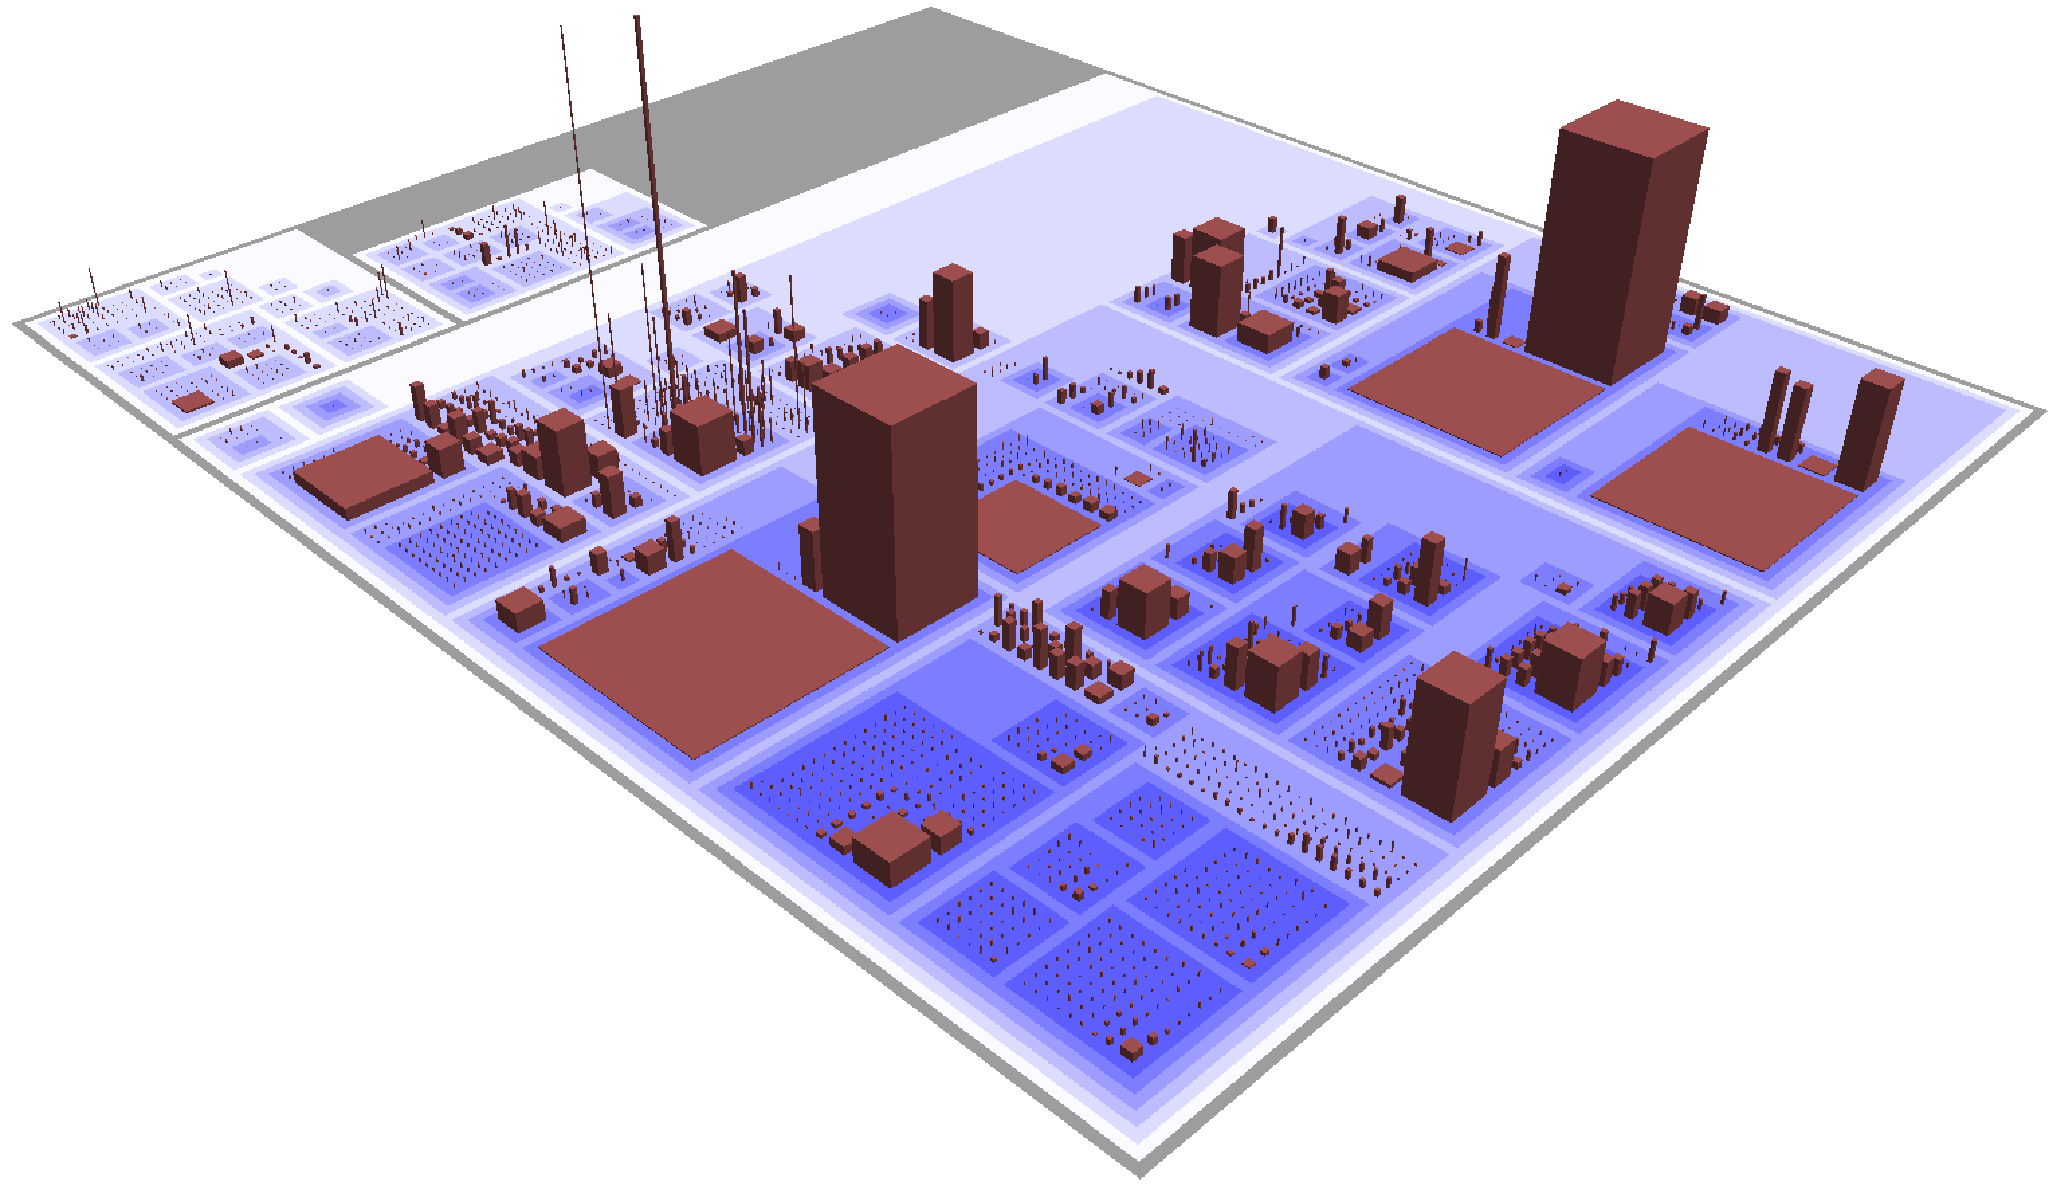
\includegraphics[width=\textwidth]{figures/code-city}
   \subcaption{CodeCity von ArgoUML \cite{wettel2008visual}} \label{fig:code-city}
  \end{subfigure}
  \hfill
  \begin{subfigure}[b]{\fwidth}
  	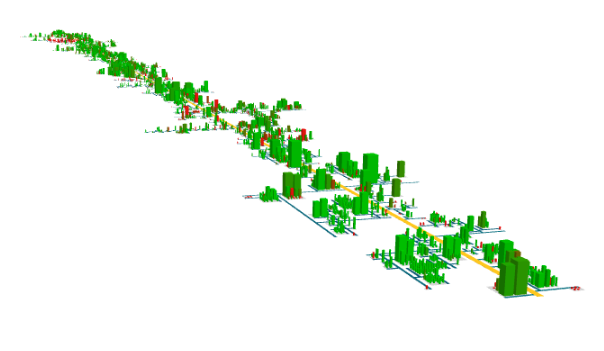
\includegraphics[width=\textwidth]{figures/softvis3d}
  	\subcaption{SoftVis3D mit Evostreet Layout} \label{fig:softvis3d}
  \end{subfigure}
  \hfill
  \vspace{1em}
  \begin{subfigure}[b]{\fwidth}
  	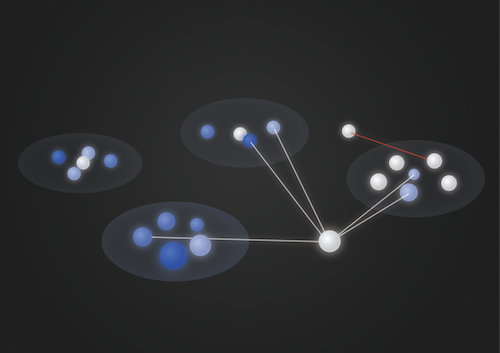
\includegraphics[width=\textwidth]{figures/code-universe}
  	\subcaption{Entwurf eines CodeUniverse} \label{fig:code-universe}
  \end{subfigure}
  \hfill
  \begin{subfigure}[b]{\fwidth}
  	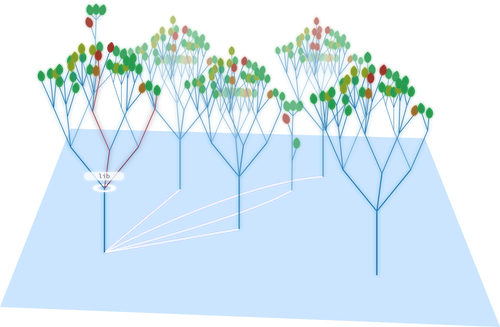
\includegraphics[width=\textwidth]{figures/code-leaves}
  	\subcaption{Erster Entwurf von CodeLeaves} \label{fig:code-leaves}
  \end{subfigure}
  \caption{CodeLeaves und alternative Ansätze der 3D Softwarevisualisierung} \label{fig:alternatives}
\end{figure}

\subsubsection*{SoftVis3D}
\textit{SoftVis3D} greift das Konzept der CodeCity auf und visualisiert als Plugin für SonarQube\footnote{SonarQube ist eine open-source Plattform für statische Code-Qualität, \url{https://www.sonarqube.org/}} Projekte direkt im Browser. Durch die direkte Anbindung an SonarQube ist SoftVis3D hoch konfigurierbar und kann alle Metriken darstellen, die auch in SonarQube zur Verfügung stehen. Neben dem \emph{District-Layout}, wie es in der CodeCity verwendet wird, unterstützt SoftVis3D darüber hinaus auch des \emph{Evostreet-Layout}, das ursprünglich in \cite{steinbruckner2013consistent} für die Evolution einer Software entworfen wurde. In diesem Layout, wie es in Abbildung \ref{fig:softvis3d} zu sehen ist, werden Pakete als sich verzweigende Straßen dargestellt. In Abbildung \ref{fig:softvis3d} fällt auf, dass die Städte mit vielen Geschwistern im root-Verzeichnis durch das Evo-Street-Layout sehr in die Länge gezogen werden, was sich negativ auf die Übersichtlichkeit auswirkt.

Die Evolution wird von SoftVis3D trotz Evostreet-Layout nicht unterstützt. Abhängigkeiten konnten in früheren Versionen aggregiert dargestellt werden. Dafür wurden Pakete im Distrikt-Layout in übereinander liegenden Ebenen abgebildet und die aggregierten Abhängigkeiten über ein zusätzliches Hilfsgebäude zu der darüberliegenden Ebene geleitet. Dadurch ging jedoch die Stadt-Metapher und die Übersichtlichkeit verloren. Die Dynamik kann in SoftVis3D ebenfalls nicht visualisiert werden. Die verwendete Technologie ist zwar mit \emph{WebGL} für den Browser State-of-the-Art, aber für die HoloLens aktuell noch nicht sinnvoll einsetzbar \cite{puetz2017softwarevisualisierung}.

\subsubsection*{CodeUniverse}

Im Zuge der der Studie \cite{puetz2017softwarevisualisierung} wurde eine weitere Metapher evaluiert. Ähnlich wie in der Arbeiten \cite{graham2004solar, balzer2004software} wird die Software als Universum dargestellt. Klassen gruppieren sich als Sterne in Galaxien. Statische Metriken können dann als Farbe und Größe der Sterne widergespiegelt werden. So können "`weiße Zwerge"' bis hin zu "`roten Riesen"' entstehen.

Das \textit{CodeUniverse} ist für statische Metriken gut geeignet. Auch die Evolution ist mit der Entstehung von neuen Sternen und Galaxien gut vorstellbar. Die Struktur der Software ist zwar mit der Gruppierung der Sterne gegeben, aber weniger offensichtlich wie andere Konzepte. Bei der Visualisierung von Abhängigkeiten und dynamischen Aufrufen stößt das CodeUniverse aber an seine Grenzen. Durch direkte Verbindungen zwischen den Sternen ist dies zwar möglich, aber bei großen Software-Systemen würde das schnell im Chaos enden. Auch in \cite{balzer2004software} wird beschrieben, dass eine übersichtliche Darstellung von Abhängigkeiten nur durch deren Aggregation erreicht werden kann. Deshalb wird in \cite{balzer2004software} ein Konzept entworfen, dass die Klassen mit einem \emph{"`hierarchischem Netz"'} verbindet. Dieses ist nichts anderes als die vorhandene Baumstruktur der Software und hat mit der Metapher des Universums auch nichts mehr zu tun. Folglich wären wir wieder bei dem neuen Konzept CodeLeaves angelangt.


\subsubsection*{Vorteile von CodeLeaves gegenüber anderen 3D Softwarevisualisierungen}
Die betrachteten Alternativen und andere haben gemein, dass sie Struktur, Dynamik und Evolution nicht vereinen. Darüber hinaus können Verbindungen zwischen Klassen nicht ohne Verlust der Übersichtlichkeit angezeigt werden. CodeLeaves soll alle drei Kategorien der Softwarevisualisierung unterstützen und ist bei der Visualisierung von Struktur und Verbindungen überlegen. Durch die Baumstruktur wie sie auch in der Software vorhanden ist, wird die Struktur eins-zu-eins wiedergegeben. Die aggregierten Abhängigkeiten lehnen sich an die Struktur an und beeinflussen diese nicht negativ. Zusätzlich zur dreidimensionalen Struktur der Bäume wird durch das Wurzelgeflecht und die Spinnweben die Dreidimensionalität sehr gut ausgenutzt.

\section{Anforderungen an CodeLeaves}
\label{sec:requirements}

Die Umfrage, die in Abschnitt \ref{sec:comparison} vorgestellt wurde, ergab einen gutes Stimmungsbarometer über die Wünsche im Bezug auf zu visualisierend Informationen. In diesem Abschnitt soll genauer auf die Anforderungen an einen CodeLeaves eingegangen werden. Dazu wurde das Konzept von CodeLeaves zwei Experten der Softwareanalyse vorgestellt und befragt was sie von CodeLeaves erwarten würden. Durch die Expertengespräche werden User-Storys gesammelt und Akzeptanzkriterien abgeleitet.

Aus der dynamischen Analyse wurde der promovierende Performance-Analyst F.\ Lautenschlager interviewt. Dieser hat im Zuge seiner Dissertation eine hochperformante Zeitreihendatenbank zur Speicherung und Auswertung von dynamischen Daten einer Software erarbeitet. Er ist führend auf diesem Gebiet und ist unter anderem als Sprecher auf internationalen Konferenzen geladen.

Als Experte der statischen Analyse wurde J.\ Weigend interviewt. Dieser ist "`Chefarchitekt, Geschäftsführer und Mitgründer der QAware. Er studierte Informatik mit Schwerpunkt \enquote*{Verteilte Systeme} an der Hochschule Rosenheim und hält dort seit 2001 Vorlesungen."' \cite{qaware2017johannes}

Die Expertengespräche werden unter Anwendung der Methoden aus \cite{cohn2004user} in User-Storys 1 - 5 zusammengefasst. Tabellen \ref{tab:acceptance1} -- \ref{tab:acceptance5} beinhalten die abgeleiteten Akzeptanzkriterien.

\begin{userstory}[u:quality]{Code-Qualität (Statik)}
  Als \textit{Softwarearchitekt}\\
  möchte ich \textit{Code-Qualität auf die Struktur abbilden können},\\
  um \textit{Anomalien und Qualitätsdefizite zu erkennen}.
\end{userstory}

\renewcommand{\arraystretch}{1.5}
\begin{tabularx}{\textwidth}{cX}
	\caption{Akzeptanzkriterien zu User-Story \ref{u:quality}} \label{tab:acceptance1}\\
	\tableheader{2}{\textbf{ID} & \textbf{Beschreibung}}
    \accid{acc:s-metrics} & Die Farbe der Blätter kann eine beliebige Metrik darstellen.\\
    \accid{acc:s-hotspots} & Ich kann Ausreißer der ausgewählten Metrik gut erkennen.\\
    \accid{acc:s-overview} & Ich möchte möglichst viele Blätter gleichzeitig betrachten können.\\
    \accid{acc:s-angle} & Ich möchte die Blätter aus allen Winkeln gut erkennen können.\\
\end{tabularx}

Die Blätter in CodeLeaves ermöglichen eine hervorragende Umsetzungsmöglichkeit von User-Story \ref{u:quality}. Sie können jegliche Metrik darstellen, seien es Zahlenwerte in Prozent oder andere Werte. Mit dem Minimum und Maximum einer ausgewählten Metrik lässt sich ein Farbverlauf festlegen mit dem die Metrik für jede Klasse gleichzeitig betrachtet werden kann und Ausreißer aus der Menge hervorstechen.

Für diese User-Story ist es besonders wichtig ein Layout für den Wald zu entwickeln, dass die Blätter so verteilt, dass sie sich so wenig wie möglich überlappen. Dieser Ansatz fließt in Kapitel \ref{ch:layout} mit ein.

\begin{userstory}[u:structure]{Kopplung und Struktur (Statik)}
  Als \textit{Softwarearchitekt}\\
  möchte ich \textit{die Kopplung und Struktur einer großen Software überblicken können},\\
  um \textit{die Zusammenhänge zu verstehen}.
\end{userstory}

\setaccid
\begin{tabularx}{\textwidth}{cX}
	\caption{Akzeptanzkriterien zu User-Story \ref{u:structure}} \\
	\tableheader{2}{\textbf{ID} & \textbf{Beschreibung}}
    \accid{acc:s-structure} & Die Struktur der Bäume spiegelt die tatsächliche Struktur der Software wider und ist gut zu erkennen.\\
    \accid{acc:s-metapher} & Ich verstehe die Metapher des Software-Waldes intuitiv.\\
    \accid{acc:s-thickness} & Die Dicke einer Kante oder Wurzel zeigt mir die Anzahl der durchfließenden Verbindungen des ausgewählten Verbindungs-Typs.\\
\end{tabularx}

Mit den Baumstrukturen und der Dicke der Kanten und Wurzeln ist User-Story \ref{u:structure} mit CodeLeaves besonders gut umsetzbar. In der AR kann der Nutzer um den Wald herum gehen, sodass er die Struktur mit den aggregierten Verbindungen aus jedem Winkel betrachten kann.

Jedoch setzten Akzeptanzkriterien \ref{acc:s-structure} - \ref{acc:s-metapher} bereits viel voraus. Aus beliebig geschachtelter Software sollen Bäume entstehen, die die Struktur korrekt wiedergeben und gleichzeitig übersichtlich sind. Überschneidungen sind zu vermeiden, da sonst die Struktur nicht eindeutig zu erkennen ist. Gleichzeitig sollen die Bäume stets natürlich wirken, was das intuitive Verständnis der Metapher fördert. Diesen Herausforderungen stellen sich die Algorithmen, die in Kapitel \ref{ch:layout} erarbeitet werden.

Akzeptanzkriterium \ref{acc:s-thickness} erfordert die Unterstützung von aggregierten Verbindungen, was in Datenmodell berücksichtigt wird.

\begin{userstory}[u:interaction]{Intuitive Erforschung (Statik)}
  Als \textit{Softwarearchitekt}\\
  möchte ich \textit{den Wald intuitiv erforschen können},\\
  um \textit{detaillierte Informationen zu erhalten}.
\end{userstory}

\setaccid
\begin{tabularx}{\textwidth}{cX}
	\caption{Akzeptanzkriterien zu User-Story \ref{u:interaction}} \\
	\tableheader{2}{\textbf{ID} & \textbf{Beschreibung}}
	\accid{acc:u-identify} & Ich kann Elemente im Wald identifizieren.\\
	\accid{acc:s-metric-value} & Ich kann mir die genaue Zahl der aktuellen Metrik für ein Blatt anzeigen lassen.\\
	\accid{acc:s-leaf-connections} & Wenn ich ein Blatt auswähle, dann kann ich die ein- bzw.\ ausgehenden Verbindungen hervorheben.\\
	\accid{acc:s-connection-count} & Wenn ich eine Kante oder Wurzel auswähle, dann kann ich sehen wie viele Verbindungen in welche Richtung fließen.\\
    \accid{acc:s-connection-highlight} & Wenn ich eine Kante oder Wurzel auswähle, dann kann ich die von den Verbindungen betroffenen Blättern hervorheben.\\
    \accid{acc:s-drilldown} & Ich kann einen Knoten als neuen Waldboden festlegen.\\
    \accid{acc:s-timestamp} & Ich kann den Zeitpunkt auswählen, auf die sich die dargestellten Daten beziehen.\\

\end{tabularx}

User-Story \ref{u:interaction} ist mit der AR sehr gut umsetzbar. Durch die AR ist der Nutzer mitten in der Visualisierung, die greifbar wird. Die Akzeptanzkriterien \ref{acc:u-identify} - \ref{acc:s-drilldown} liefern für die Interaktion mit CodeLeaves eine wertvolle Basis und werden in Kapitel \ref{ch:interaction} aufgegriffen.

\begin{userstory}[u:dynamic]{Dynamische Daten}
  Als \textit{Performance-Analyst}\\
  möchte ich \textit{Funktionsaufrufe, deren Antwortzeiten, Laufzeitfehler und Ressourcen-Auslastung visualisiert haben},\\
  um \textit{das Laufzeitverhalten der Software in einem bestimmten Zeitraum explorativ bewerten zu können.}
\end{userstory}

\setaccid
\begin{tabularx}{\textwidth}{cX}
	\caption{Akzeptanzkriterien zu User-Story \ref{u:dynamic}} \\
	\tableheader{2}{\textbf{ID} & \textbf{Beschreibung}}
    \accid{acc:d-metrics} & Die Farbe der Blätter kann eine beliebige Metrik darstellen.\\
    \accid{acc:d-hotspots} & Ich kann Ausreißer der ausgewählten Metrik gut erkennen.\\
     \accid{acc:d-thickness} & Die Dicke einer Kante oder Wurzel zeigt mir die Anzahl der durchfließenden Verbindungen des ausgewählten Verbindungs-Typs.\\
    \accid{acc:d-metric-value} & Ich kann mir die genaue Zahl der aktuellen Metrik für ein bestimmtes Blatt anzeigen lassen.\\
    \accid{acc:d-leaf-connections} & Wenn ich ein Blatt auswähle, dann kann ich die ein- bzw.\ ausgehenden Verbindungen hervorheben.\\
    \accid{acc:d-connection-highlight} & Wenn ich eine Kante oder Wurzel auswähle, dann kann ich die von den Verbindungen betroffenen Blättern hervorheben.\\
    \accid{acc:d-connection-count} & Wenn ich eine Wurzel oder Kante auswähle, dann kann ich sehen wie viele Verbindungen in welche Richtung gehen.\\
    \accid{acc:d-timespan} & Ich kann den Zeitraum auswählen, auf die sich die dargestellten Daten beziehen.\\
    \accid{acc:d-add-info} & Ich kann zusätzliche Informationen über den Wald als Ganzes visualisieren.\\
\end{tabularx}

Durch User-Story \ref{u:dynamic} wird deutlich, dass sich viele gleiche Akzeptanzkriterien aus statischen und dynamischen User-Storys ableiten lassen. Daran ist zu erkennen wie sinnvoll es ist diese beiden Sichten miteinander zu kombinieren. Ob es sich um statische oder dynamische Daten handelt, spielt für die Visualisierung großteils keine Rolle. Es ändert sich lediglich der betrachtete Zeitpunkt bei statischen Daten zu einem Zeitraum für dynamische Daten. Die Ressourcen-Auslastung sind zusätzliche Informationen, die den Wald als Ganzes betreffen und werden im Datenmodell berücksichtigt.

\begin{userstory}[u:overview]{Zustand der Software (Dynamik)}
  Als \textit{Systemverantwortlicher}\\
  möchte ich \textit{auf einen Blick den Zustand meiner Software erkennen},\\
  um \textit{bei Bedarf agieren zu können}.
\end{userstory}

\setaccid
\begin{tabularx}{\textwidth}{cX}
	\caption{Akzeptanzkriterien zu User-Story \ref{u:overview}} \label{tab:acceptance5}\\
	\tableheader{2}{\textbf{ID} & \textbf{Beschreibung}}
    \accid{acc:d-overview} & Wenn ich die Laubfarbe des Waldes betrachte, dann möchte ich eine möglichst gute Gesamtübersicht über die ausgewählte Metrik haben.\\
    \accid{acc:d-overview} & Ich möchte möglichst viele Blätter gleichzeitig betrachten können.\\
\end{tabularx}

User-Story \ref{u:overview} weißt wiederum Ähnlichkeiten zu User-Story \ref{u:overview} auf. Die Laubfarbe ist auch für den Systemzustand sehr gut geeignet, da sie eine gute Übersicht liefert, aber gleichzeitig jede Klasse einzeln anzeigt. Die Metapher des Software-Waldes kommt auch hier besonders zur Geltung, da auf einen Blick ersichtlich wird, ob es der Software gut geht (sommerlicher Wald) oder schlecht (herbstlicher Wald).

\subsubsection*{User-Storys zur Benutzbarkeit von CodeLeaves}

Aus anfänglichem Prototyping mit in der AR sind weitere User-Story entstanden, ohne die die anderen erst gar nicht möglich sind. Somit werden User-Storys \ref{u:adjust} und \ref{u:project-selection} und deren Akzeptanzkriterien in Tabellen \ref{tab:acceptance6} und \ref{tab:acceptance7} im Folgenden beschrieben.

\begin{userstory}[u:adjust]{Anpassung im Raum (Nutzbarkeit)}
  Als \textit{Nutzer} in der AR\\
  möchte ich \textit{den Wald meinen Räumlichkeiten und Wüschen anpassen können},\\
  um \textit{den Wald sinnvoll nutzen zu können}.
\end{userstory}

\setaccid
\begin{tabularx}{\textwidth}{cX}
	\caption{Akzeptanzkriterien zu User-Story \ref{u:adjust}} \label{tab:acceptance6}\\
	\tableheader{2}{\textbf{ID} & \textbf{Beschreibung}}
    \accid{acc:u-place} & Ich kann den Wald im Raum platzieren.\\
    \accid{acc:u-scale} & Ich kann den Wald skalieren.\\
    \accid{acc:u-rotate} & Ich kann den Wald rotieren.\\
\end{tabularx}

Vor allem am Anfang der Nutzung von CodeLeaves ist es wichtig den Wald dorthin zu platzieren, wo es am meisten Sinn macht. Ist der Wald initial von realen Objekten verdeckt, kann der Nutzer nicht damit arbeiten. Für den Wechsel zwischen Übersicht und der Betrachtung von Details ist es essentiell die Größe des Waldes jederzeit einfach anpassen zu können. Die Rotation des Waldes kann komfortabler sein, als um den ganzen Wald herum zu laufen.

Vor der Platzierung des Waldes ist noch ein weiterer Schritt erforderlich. Es muss als erstes ein Projekt ausgewählt werden können, das dargestellt werden soll. Die letzte User-Story beschreibt deshalb die Auswahl bzw.\ den Import von Projekten und Tabelle \ref{tab:acceptance7} deren Akzeptanzkriterien.

\begin{userstory}[u:project-selection]{Auswahl eines Projekts (Nutzbarkeit)}
  Als \textit{Nutzer}\\
  möchte ich \textit{ein bestehendes Projekt öffnen und neue importieren können},\\
  um \textit{das Projekt zu betrachten, das mich interessiert}.
\end{userstory}

\setaccid
\begin{tabularx}{\textwidth}{cX}
	\caption{Akzeptanzkriterien zu User-Story \ref{u:project-selection}} \label{tab:acceptance7}\\
	\tableheader{2}{\textbf{ID} & \textbf{Beschreibung}}
    \accid{acc:u-project-selection} & Ich kann bereits gespeicherte Projekte öffnen.\\
    \accid{acc:u-import} & Ich kann ein neues Projekt aus unterstützen Datenquellen importieren.\\
    \accid{acc:u-add-data} & Ich kann Daten zu einem bereits gespeicherten Projekt aus unterstützen Daten hinzufügen.\\
\end{tabularx}

Akzeptanzkriterium \ref{acc:u-project-selection} ist für einen vollständigen technischen Durchstich wichtig, da so in der HoloLens Applikation ein Beispielprojekt geöffnet werden kann.

User-Storys \ref{u:quality} - \ref{u:overview} sind auf High-Level-Ebene formuliert. Viele der Akzeptanzkriterien finden jedoch schon im Prototyping Anwendung. Im weitern Verlauf des Textes wird deshalb bei der Adressierung eines Akzeptanzkriteriums in folgender Form darauf verwiesen: \textit{(Akz. <ID>)}.

Im nächsten Kapitel wird ein Datenmodell entworfen, mit dem alle vorgestellten User-Storys umgesetzt werden können.

\chapter{Datenmodell}
\label{ch:data-model}
\section{Trennung in Schichten}
\label{ch:data-layers}

Das Datenmodell für CodeLeaves nimmt einen zentralen Baustein ein, auf den sich der Prototyp für die HoloLens stützt. Bei dem Entwurfsmuster wird ein wichtiges Prinzipien beachtet. Wie Buschmann et al. in \cite{frank2007pattern} beschreibt, ist das Pattern \textit{Layers} ein Grundprinzip bei Software-Architekturen. Durch die \textit{Separation of concerns} werden einzelnen Schichten voneinander getrennt und können so später leichter ausgetauscht werden: ``Using semi-independent parts [...] enables the easier exchange of individual parts at a later date.`` \cite{frank2007pattern}

\subsubsection*{Backend}
Gerade bei der Visualisierung von abstrakten Daten, wie es eine Software ist, ist eine Schichtentrennung besonders wichtig. CodeLeaves hat das Ziel eine beliebige objektorientierte Software darstellen zu können. Da aber nicht für jede Programmiersprache CodeLeaves angepasst werden soll und die Informationen über die Software aus unterschiedlichen Quellen stammen können, ist hier die erste Schicht \textit{Backend} sinnvoll. In der Backend Schicht werden die Daten über eine Software aggregiert, seien es statische oder dynamische Informationen und in ein Sprach-agnostisches Format -- dem \textit{Software-Meta-Modell} -- gebracht. So können beliebig viele Konnektoren, d.h. die Verbindungen zu den verschiedenen Datenquellen, implementiert werden.

Wie in Abschnitt \ref{sec:distinction} bereits festgehalten, soll der Schritt des Transfers der realen Software in deren abstrakte Repräsentation jedoch nicht Schwerpunkt dieser Arbeit sein. Das Datenmodell ist hingegen sehr wohl zu definieren, um die Daten darstellen zu können.

\subsubsection*{Application-logic}
Die Einteilung in Schichten geht nach der Transformation der Software in ein Meta-Modell weiter. CodeLeaves könnte neben Software prinzipiell auch jegliche anderen, hierarchisch strukturierten Informationen darstellen. Für die interne Datenhaltung wird deshalb in der Schicht \textit{Application-logic} das Datenmodell weiter abstrahiert und in ein Format gebracht, dass sich stark an der Baumstruktur der Informatik orientiert und nicht rein auf Software zugeschnitten ist. So könnten später auch leicht gänzlich andere Daten angebunden werden. Wir nennen das Datenmodell dieser Schicht das \textit{interne Datenmodell}.

\subsubsection*{Presentation}
Die letzte Schicht ist die der \textit{Presentation}. Das interne Datenmodell wird für die Darstellung der Bäume weiter verarbeitet. Zum Beispiel muss für die Layout-Algorithmen die Höhe der einzelnen Knoten verfügbar sein. Dies sind aber Informationen, die nur von der UI benötigt werden und im internen Datenmodell nichts zu suchen haben. Auf der anderen Seite enthält das \textit{UI-Datenmodell} nur Informationen, die auch tatsächlich zum Rendern der 3D Objekte benötigt werden.

Diese Schicht könnte wieder ausgetauscht werden und unterschiedliche Layout-Algorithmen könnten unterstützt werden.

In Abbildung \ref{fig:data-layers} ist die Beziehung der Datenmodelle in den drei Schichten abgebildet.

\begin{figure}[htb]
  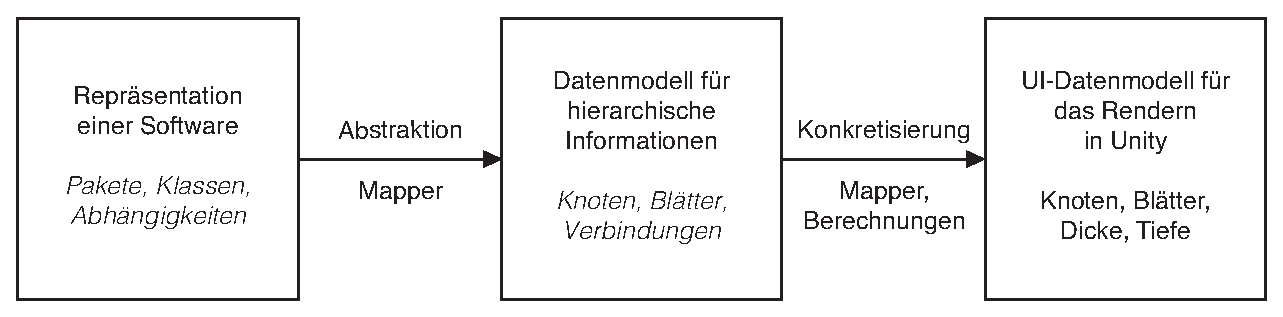
\includegraphics[width=\textwidth]{\figdir/data-layers}
  \caption{Schichtentrennung im Datenmodell}
  \label{fig:data-layers}
\end{figure}

\section{Software-Meta-Modell}
\label{sec:software-model}

\subsubsection*{Vorhandene Meta-Modelle}

CodeCity verwendet als Meta-Modell für Software das sogenannte \textit{FAMIX}-Modell in Version 2.1. Dieses wird bis heute von \textit{Moose}, dem Software-Analyse-Tool, auf dem CodeCity basiert, protegiert und ist heute in Version 3.0 verfügbar \cite{merrill1916moose}. Das Meta-Modell ist sehr umfangreich und beinhaltet 51 verschiedene Entities. Es wird in einem eigenen Dateiformat namens MSE, vergleichbar mit JSON oder XML, gespeichert. Da aber dynamische Informationen nicht im FAMIX-Modell enthalten sind, eignet sich das Format nicht um in CodeLeaves verwendet zu werden.

Ein Meta-Modell, das dynamische und statische Informationen vereint, existiert nach heutigem Wissensstand nicht.

Für eine reine dynamische Analyse ist das Tool \textit{ExplorVis} sehr ausgereift \cite{fittkau2017software}. Das im nachfolgende entwickelte Meta-Modell ist von Aspekten aus dem FAMIX- und dem ExplorVis-Modell inspiriert. Dabei soll das Modell aber möglichst simpel gehalten werden und nur das beinhalten, was CodeLeaves auch darstellen kann.

\subsubsection*{Entwicklung eines eigenen Modells}

Um uns vor Augen zu führen, welche Informationen relevant sind, rufen wir uns die User-Storys aus Kapitel \ref{ch:concept} in Erinnerung.

Aus den User-Storys \ref{u:quality} und \ref{u:dynamic} ergeben sich folgende Metriken, die das Software-Meta-Modell unterstützen muss:

\begin{itemize}
  \item Statische Metriken zur Code-Qualität
  \item Antwortzeiten
  \item Laufzeitfehler
\end{itemize}

Aus User-Story \ref{u:structure} und \ref{u:dynamic} gehen folgende Verbindungen hervor:

\begin{itemize}
  \item Statische Abhängigkeiten
  \item Dynamische Aufrufe
\end{itemize}

Diese Metriken und Verbindungen müssen auf die Struktur der Software abgebildet werden. Damit lässt sich das Modell einer Software, ob statisch oder dynamisch betrachtet, auf drei wesentliche Elemente reduzieren:

\begin{enumerate}
  \item Struktur
  \item Metriken
  \item Verbindungen
\end{enumerate}

Diese drei Elemente sind in Abbildung \ref{fig:meta-model} mit den Klassen \texttt{SoftwareArtefact}, \texttt{Metric} und \texttt{Relation} zu finden. Für den besseren Lesefluss wird im Folgenden auf den Zusatz "`\dots-Klasse"' verzichtet.

Die \texttt{Metric} ist ein Schlüssel-Wert-Paar, das durch \texttt{Codesnippets} ergänzt werden kann. So ist es zum Beispiel möglich bei Laufzeitfehler zu sehen, an welcher Stelle die Fehler aufgetreten sind. Der \texttt{Key} identifiziert die Metrik, wie zum Beispiel statische Testabdeckung oder dynamische Laufzeitfehler und der \textit{Value} enthält die Zahl, die dann in die Farbe der Blätter umgewandelt werden kann.

%\begin{figure}[htb]
%  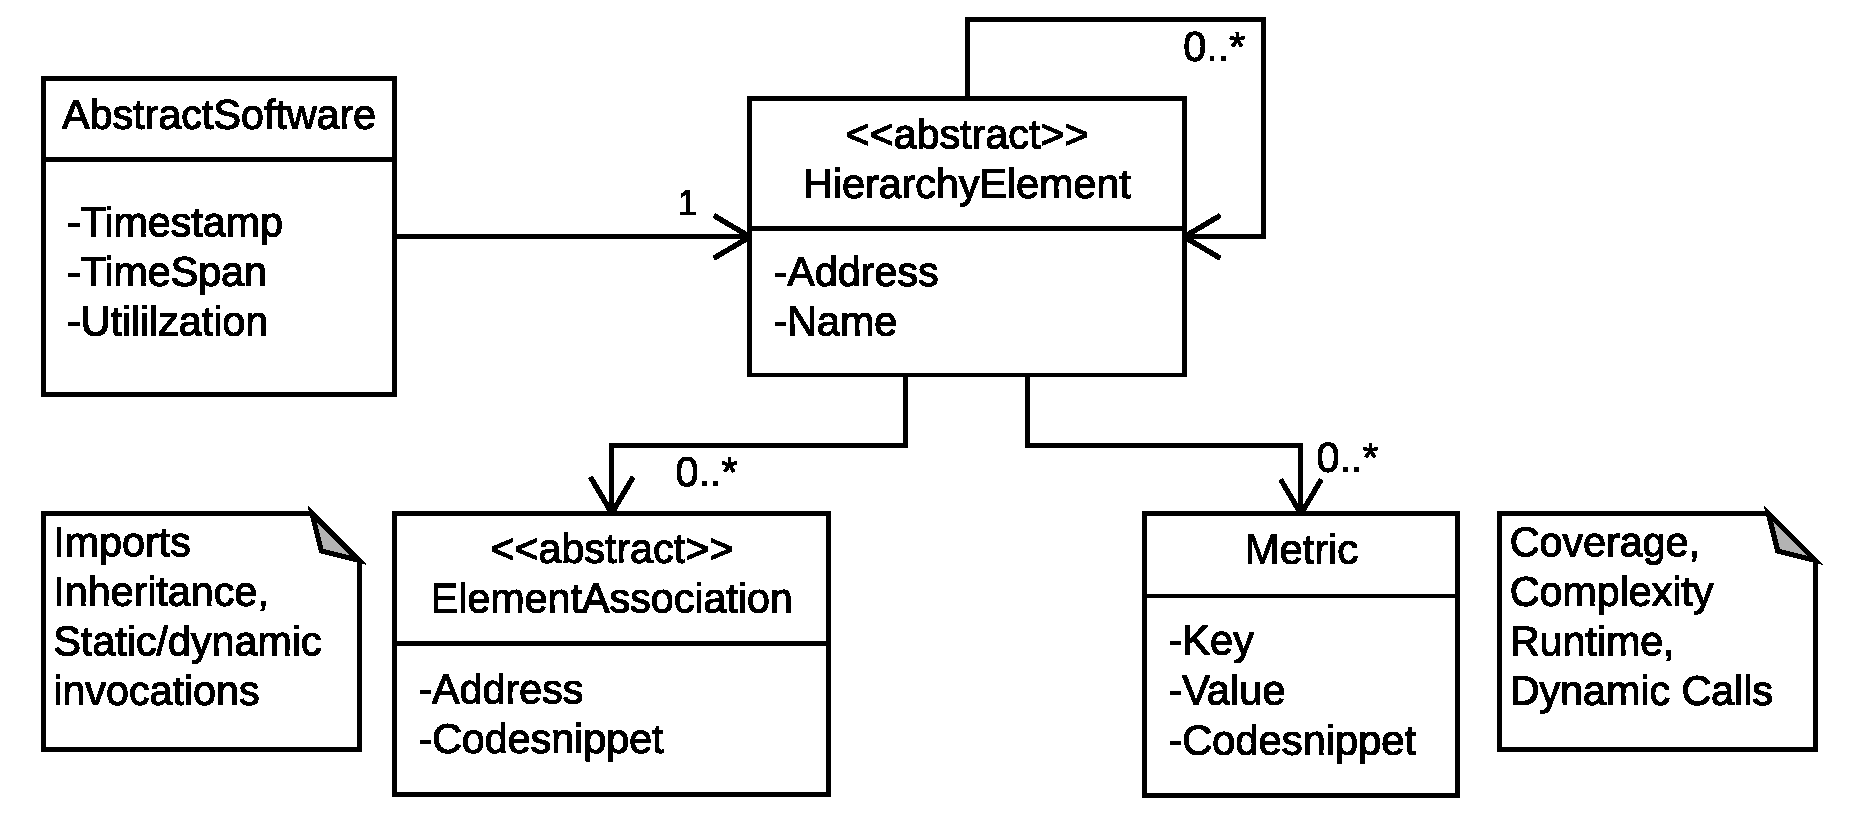
\includegraphics[scale=0.5]{\figdir/meta-model}
%  \caption{Meta-Modell einer Software}
%  \label{fig:meta-model}
%\end{figure}

\begin{figure}[htb]
\begin{tikzpicture}
  \umlsimpleclass[x=-6]{Software}
  \umlsimpleclass[type=abstract]{Record}
  \umlclass[x=6, y=1.5]{StaticRecord}{
    Timestamp \\
  }{}
  \umlclass[x=6, y=-1.5]{DynamicRecord}{
    Timespan \\
    Utilization \\
  }{}
  \umlclass[y=-5, x=6]{Metric}{
    Key \\
    Value \\
    Codesnippets \\
  }{}
  \umlclass[y=-5]{SoftwareArtefact}{
    Key \\
    Name \\
  }{}
  \umlclass[y=-5, x=-6]{Relation}{
    Key \\
    Type \\
    Start \\
    End \\
  }{}
  \umluniassoc[mult=0..*]{Software}{Record}
  \umlinherit[geometry=-|-]{StaticRecord}{Record} 
  \umlinherit[geometry=-|-]{DynamicRecord}{Record}
  \umluniassoc[geometry=|-|, mult=1, pos=2.6]{Record}{SoftwareArtefact}
  \umluniassoc[mult=0..*]{SoftwareArtefact}{Metric}
  \umluniassoc[geometry=|-|, mult=0..*, pos=2.6]{Record}{Relation}
  \umluniassoc[mult=0..*, angle1=-120, angle2=180, loopsize=2cm]{SoftwareArtefact}{SoftwareArtefact}
\end{tikzpicture}
\caption{Meta-Modell einer Software}
\label{fig:meta-model}
\end{figure}

Die Struktur wird im Software-Meta-Modell nicht wie in den anderen beiden Schichten mit einem Kompositum-Muster entworfen, sondern nur mit dem \texttt{SoftwareArtefact}, das eine Liste von Kindern besitzt. Diese Liste ist für eine Klasse leer. Grund für diese Modellierung ist die leichtere Serialisierung. Das Kompositum-Muster, wie es in den andern beiden Schichten Verwendung findet, beinhaltet eine abstrakte Klasse, die das Blatt und das Kompositum spezialisieren. Für die Deserialisierung müssten bei der Erzeugung von Objekten Zusatzinformationen angegeben werden, ob es sich um ein Blatt, oder ein Kompositum handelt. Mögliche Datenquellen wie SonarQube haben in ihrem Modell für die Struktur ebenfalls nur eine Klasse, wodurch die Logik beim Import der Daten möglichst gering gehalten wird.

Analog zur Definition \ref{def:softwareartefact} spielt es bei einem \texttt{SoftwareArtefact} keine Rolle, wie die Software organisiert ist. Egal ob ein ganzes Projekt, Paket oder eine einzelne Methode, alles wird zu einem Softwareartefakt.

Jedes \texttt{SoftwareArtefact} besitzt einen für den Nutzer lesbaren Namen und einen eindeutigen Schlüssel, mit dem es eindeutig identifiziert werden kann. Daneben beinhaltet ein \texttt{SoftwareArtefact} beliebig viele Objekte des Klasse \texttt{Metric}. Werden diese jedoch einem \texttt{SoftwareArtefact} mit Kinder, d.\,h.\ einem Paket zugeordnet, finden sie in der weiteren Verarbeitung keine Relevanz, da in CodeLeaves für innere Knoten keine Metriken vorgesehen sind.

Mit der \texttt{Relation} können Verbindungen in einer Software wie statische Abhängigkeiten oder dynamische Aufrufe gespeichert werden. Der \texttt{Type} gibt die Art der Verbindung an. Eine \texttt{Relation} ist nicht direkt mit einem \texttt{SoftwareArtefact} assoziiert, um zyklische Abhängigkeiten im Datenmodell zu vermeiden. Stattdessen werden Start- und Endpunkt der Verbindung mit den Schlüsseln der verbundenen Klassen angegeben.

Durch die Expertengespräche ging hervor, dass sowohl bei Metriken als auch bei Verbindungen ein Bezug zum Code wichtig ist. Demnach beinhaltet die Klasse \texttt{Relation} ebenfalls die Möglichkeit \texttt{Codesnippets} zu speichern, sodass ersichtlich wird, wo im Code die Verbindung ihren Ursprung hat.

Neben Struktur, Metriken und Verbindungen einer Software muss der Zeitraum bzw.\ der Zeitpunkt angegeben werden können. Damit wird auch die Evolution einer Software zu unterstützt.

Deshalb werden Struktur und Verbindungen in einem Datensatz -- dem \texttt{Record} -- gespeichert. Eine Software wiederum kann beliebig viele Datensätze enthalten. Bei einem Datensatz muss zwischen einem statischem und einem dynamischen unterschieden werden. Bei statischen Daten wird nur ein bestimmter Zeitpunkt betrachtet, bei dynamischen ist es dagegen ein bestimmter Zeitraum. Daraus resultiert, dass ein \texttt{Record} von einem \texttt{StaticRecord} und einem \texttt{DynamicRecord} spezialisiert wird.

Aus User-Story 1 geht hervor, dass es bei dynamischen Daten gilt auch die Ressourcen-Auslastung zu visualisieren. Die Informationen dazu können im \texttt{DynamicRecord} in \texttt{Utilization} gespeichert werden.

\section{Internes Datenmodell}
\label{sec:app-model}

Wie in Abbildung \ref{fig:internal-model} zu sehen, ist das interne Datenmodell sehr ähnlich zu dem des Software-Meta-Modells. Das Modell ist zunächst die semantische Transformation einer Software in ein Format, das beliebige hierarchische Daten darstellt. So wird beispielsweise \texttt{Software} zum \texttt{Forest}, eine \texttt{Relation} zur \texttt{Connection} und eine \texttt{Metric} zu \texttt{LeafData}.

Neben der semantischen Transformation wird das \texttt{SoftwareArtefact} durch ein Kompositum-Pattern mit \texttt{Node}, \texttt{InnerNode} und \texttt{Leaf} ersetzt. Mit der Methode \texttt{Find} wird das Suchen eines Knotens in den Spezialisierungen von \texttt{Node} implementiert. Die Metriken aus dem Software-Meta-Modell sind im internen Datenmodell nur noch bei Blättern verfügbar.

\begin{figure}[htb]
\begin{tikzpicture}
  \umlsimpleclass[x=-5.7]{Forest}
  \umlclass[type=abstract]{Record}{
    AdditionalData \\
  }{}
  \umlclass[x=5.7]{Moment}{
    Timestamp \\
  }{}
  \umlclass[x=5.7, y=-2.5]{Period}{
    Timespan \\
  }{}
  \umlclass[y=-5]{Node}{
    Key \\
    Name \\
  }{
    \textit{Find()}
  }
  \umlclass[y=-10, x=-1.8]{InnerNode}{
  }{
    Find()
  }
  \umlclass[y=-10, x=1.8]{Leaf}{
  }{
    Find()
  }
  \umlclass[y=-10, x=5.7]{LeafData}{
    Key \\
    Value \\
    AdditionalData\\
  }{}
  \umlclass[y=-5, x=-5.7]{AggregatedConnection}{
    Type \\
    Key \\
    Start \\
    End \\
  }{}
  \umlclass[y=-10, x=-5.7]{Connection}{
    Key \\
    Start \\
    End \\
  }{}
  \umluniassoc[mult=0..*]{Forest}{Record}
  \umlinherit{Moment}{Record}
  \umlinherit[geometry=-|-]{Period}{Record}
  \umluniassoc[geometry=|-|, mult=1, pos=2.5]{Record}{Node}
  \umluniassoc[geometry=|-|, mult=0..*, pos=2.5]{Record}{AggregatedConnection}
  \umlunicompo[mult=1..*]{AggregatedConnection}{Connection}
  \umluniassoc[geometry=|-, mult=0..*, anchor1=120, anchor2=180]{InnerNode}{Node}
  \umlinherit[geometry=|-|]{InnerNode}{Node}
  \umlinherit[geometry=|-|]{Leaf}{Node}
  \umluniassoc[mult=0..*]{Leaf}{LeafData}
\end{tikzpicture}
  \caption{Internes Datenmodell}
  \label{fig:internal-model}
\end{figure}

Beim Transfer in das interne Datenmodell werden ebenfalls die einzelnen Verbindungen aggregiert. Eine \texttt{AggregatedConnection} besteht mindestens aus einer direkten Verbindung.

Die \texttt{Utilization} aus dem \texttt{DynamicRecord} wandert als \texttt{AdditionalData} in die den abstrakten \texttt{Record}, da bei andern hierarchischen Daten eventuell auch für einen Zeitpunkt zusätzliche Daten relevant sein könnten.

Die Multiplizität zwischen \texttt{InnerNode} und \texttt{Node} wird mit $0..*$ angegeben, was der klassischen Definition eines inneren Knoten (vgl. \ref{sec:naming}) widerspricht. Jedoch kann es auch bei Ausnahmefällen auch vorkommen, dass ein Softwareartefakt weder Daten, noch Kinder besitzt. Bei einem leeren Paket ohne weitere Unterpakete und Klassen wäre das der Fall. Mit der angegebenen Multiplizität kann das Datenmodell auch mit diesen Fällen umgehen. In der Visualisierung resultiert daraus eine Kante ohne Blatt.

In Abbildung \ref{fig:internal-model} wurden nur Klassen berücksichtigt, die auch Daten zur Software enthalten. Über die Datensätze zur Software hinaus, werden für den internen Zustand von CodeLeaves weitere Informationen benötigt. Beispielsweise muss gespeichert werden, welche Metriken aktuell angezeigt werden. Einen Eindruck über die Einstellungen, die der Nutzer in CodeLeaves vornehmen kann, wird in Kapitel \ref{ch:interaction} ausgeführt.

\section{UI-Datenmodell}
\label{sec:hierarchical-model}

Das UI-Datenmodell ist stark von der Praxis des Prototypings mit der HoloLens beeinflusst. Es wurde darauf geachtet, dass das Modell nur Daten beinhaltet, das auch zwangsläufig für das Rendern der Visualisierung nötig ist.

Das ist bei einem Blatt die Farbe und bei einem inneren Knoten die Dicke der dazugehörigen Kante. Beide Spezialisierungen eines \texttt{UiNode} beinhalten zusätzlich einen beliebigen Text, der abhängig von der Interaktion des Nutzers ist. Zusätzlich sind mit \texttt{isHighlighted} und \texttt{isSelected} zwei Zustände gegeben, denen entsprechend die Darstellung des Knotens angepasst werden muss. Wie die Reaktion auf Zustandsänderungen im UI-Datenmodell mit reaktiver Programmierung technisch sinnvoll umgesetzt werden kann, ist in Kapitel \ref{ch:interaction-ar} zu finden.

In Abbildung \ref{fig:ui-model} ist das UI-Datenmodell zu sehen.

%\begin{figure}[htb]
%  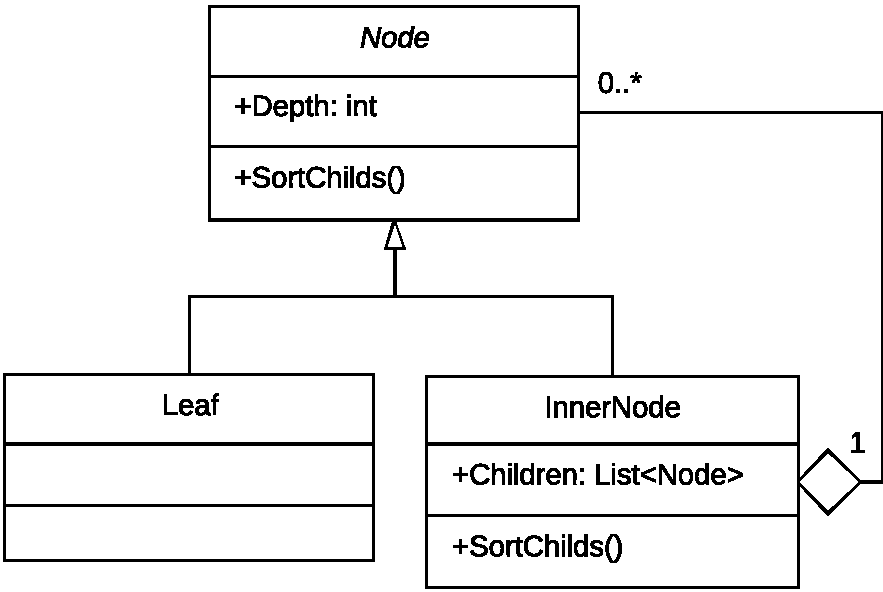
\includegraphics[width=.6\textwidth]{\figdir/ui-model}
%  \caption{UI-Datenmodell}
%  \label{fig:ui-model}
%\end{figure}

\begin{figure}[htb]
\begin{tikzpicture}
  \umlsimpleclass[x=-8]{UiForest}
  \umlclass{UiNode}{
    Key \\
    Text \\
    IsHighlighted \\
    IsSelected \\
    \textit{Circle}
  }{
    \textit{Find()}\\
    \textit{GetHeight()}\\
    \textit{GetDescendantsCount()}\\
    \textit{SortChildren()}\\
  }
  \umlclass[y=-7, x=-3]{UiInnerNode}{
    Thickness \\
    Circle \\
  }{
    Find()
    GetHeight()\\
    GetDescendantsCount()\\
    SortChildren()\\
  }
  \umlclass[y=-7, x=3]{UiLeaf}{
    Color \\
    Circle
  }{
    Find()
    GetHeight()\\
    GetDescendantsCount()\\
    SortChildren()\\
  }
  \umluniassoc[geometry=-|, mult=0..*, anchor2=110, pos2=2.8]{UiForest}{UiInnerNode}
  \umluniassoc[geometry=|-, mult=1..*, anchor2=180]{UiInnerNode}{UiNode}
  \umlinherit[geometry=|-|, arm1=0.5, anchor1=70]{UiInnerNode}{UiNode}
  \umlinherit[geometry=|-|, arm1=0.5, anchor1=110]{UiLeaf}{UiNode}
\end{tikzpicture}
\caption{UI-Datenmodell}
\label{fig:ui-model}
\end{figure}

Die \texttt{AdditionalData} aus dem internen Datenmodell finden sich in dem Entwurf des UI-Datenmodells nicht wieder. Grund dafür ist, dass der Kern der Visualisierung davon nicht betroffen ist. Die Anzeige dieser Daten kann beliebig zum Wald dargestellt werden.

Auf den \texttt{Circle} bzw.\ dem \textit{Kreis} eines Knotens, wird im Zuge des Layouts im nächsten Kapitel eingegangen. Für das Layout ist es außerdem nötig die Knoten sortieren zu können. Die abstrakten Methoden von \texttt{UiNode} sind dazu erforderlich und werden entsprechend in \texttt{UiInnerNode} und \texttt{UiLeaf} realisiert.

% ----===== Chapter ====---- %
\chapter{Modellierung und Layout des Waldes}
\label{ch:layout}

\section{Grundlegender Ansatz}

CodeLeaves steht und fällt mit der korrekten und übersichtlichen Darstellung der Baumstruktur. Wegen Akzeptanzkriterien \ref{acc:s-overview} und \ref{acc:d-overview} ist die Struktur der Bäume so zu generieren, dass so viele Blätter wie möglich gleichzeitig im Blickfeld des Betrachters sind. Auf der anderen Seite gilt es wegen Akzeptanzkriterien \ref{acc:s-structure} und \ref{acc:d-overview} die Struktur übersichtlich und deswegen mit so wenig Überschneidungen wie möglich zu generieren. In Abschnitt \ref{sec:sunflower} und \ref{sec:Circle-Packing} werden deshalb zwei Algorithmen vorgestellt, die zusammen eine solche Darstellung der Baumstruktur ermöglichen. 

\subsubsection*{Prototypen}

Die Algorithmen werden in einem \textit{High-Fi Prototyp}\footnote{englisch High Fidality, aus: high = hoch und fidelity = Genauigkeit; High-Fi Prototypen zeichnen sich durch eine High-Tech-Darstellung der Designkonzepte aus, die zu einer partiellen bis vollständigen Funktionalität führt \cite{egger2000fi}.} für die HoloLens implementiert. Der High-Fi Prototyp ist wichtig, da nur damit CodeLeaves in der AR erlebt werden kann. Auch die wichtigsten Interaktionen, die im Kapitel \ref{ch:interaction} beschrieben werden, können im High-Fi Prototyp schon getestet werden. Weitere Interaktions-Elemente werden in Kapitel \ref{ch:interaction} mit einem Papier \textit{Low-Fi Prototyp}\footnote{englisch Low Fidality, aus: low = gering und fidelity = Genauigkeit; Low-Fi Prototypen zeichnen sich durch eine schnelle und einfache Übersetzung von Designkonzepten auf hohem Niveau in greifbare und testbare Artefakte aus \cite{egger2000fi}.} ergänzt.

Bei dem High-Fi Prototyp wird auf den Standard-Workflow der HoloLens-Entwicklung gesetzt. HoloLens-Applikationen werden in \textit{Unity}\footnote{https://unity3d.com/de} entwickelt. Unity ist eine platt\-form\-über\-grei\-fen\-de 2- und 3D Game-Engine und nach eigenen Angaben \textit{"`Die weltweit führende Software der Game-Industrie"'} \cite{unity2017public}. d

Für die HoloLens wird die Position der Hauptkamera in Unity auf die Position der HoloLens übertragen. Hologramme entstehen durch normale 3D Objekte in Unity. Diesen Objekten können Skripte zugewiesen werden, die zur Laufzeit ausgeführt werden. Die verwendete Skript-Sprache im Prototyp von CodeLeaves is C\#.

Für die Generierung von Bäumen mussten zunächst 3D Objekte entworfen werden, die die Knoten und Blätter repräsentieren. Dies wurde nicht in Unity, sondern mithilfe des professionellen 3D Modellierungs-Software Maya\footnote{https://www.autodesk.de/products/maya/overview} von Audodesk bewerkstelligt.

\subsubsection*{3D Objekte}

Die Bäume für CodeLeaves kommen mit den Objekten Kante und Blatt aus. Ein innerer Knoten wird der Baum Metapher folgend immer durch die Kante zum Elternteil bzw.\ zum Waldboden dargestellt.

\paragraph{Kanten-Objekt} Eine Kanten-Objekt ist ein vertikal ausgerichteter, nach oben leicht zulaufender Zylinder was die Abbildung \ref{fig:edge} veranschaulicht ist. Die Pivots zur Position, Rotation und Skalierung wurden so gewählt, dass eine Manipulation des Objekts immer um den Mittelpunkt der Grundfläche erfolgt.\\

\paragraph{Blatt-Objekt} Das Blatt-Objekt wurde als Abstraktion eines echten Blattes modelliert und ist in Abbildung \ref{fig:leaf} zu sehen.\\

\setlength{\fwidth}{.3\textwidth}
\begin{figure}[htb]
  \centering
  \begin{subfigure}[b]{\fwidth}
   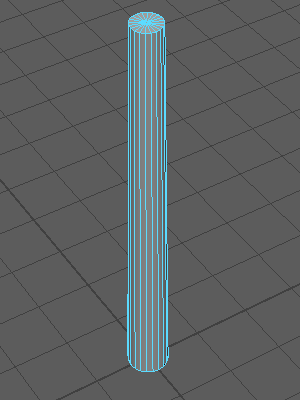
\includegraphics[width=\textwidth]{figures/edge}
   \subcaption{Kante} \label{fig:edge}
  \end{subfigure}
  \hspace{.5 cm}
  \begin{subfigure}[b]{\fwidth}
  	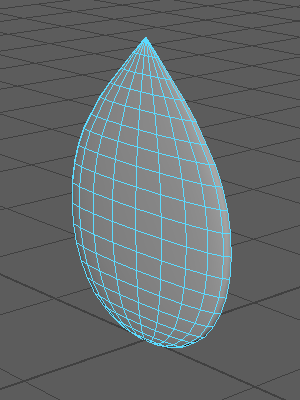
\includegraphics[width=\textwidth]{figures/leaf}
  	\subcaption{Blatt} \label{fig:leaf}
  \end{subfigure}
  \caption{3D Objekte für den High-Fi Prototyp} \label{fig:3d-objects}
\end{figure}

Das Blatt-Objekt hat aufgrund der flachen Form die Eigenschaft, dass die sichtbare Fläche bei seitlicher Betrachtung deutlich geringer ist als von vorne. Wir stellen uns einen Baum vor, bei dem der Betrachter nur die Kanten der Blätter sieht. Dadurch lassen sich die Farben der Blätter nur schwer miteinander vergleichen. Dies sollte aber aus jedem Winkel möglich sein (Akz. \ref{acc:s-angle}).

Eine Abhilfe könnte ein Blatt-Objekt sein, dass in allen Dimensionen gleich dick ist. Dies würde aber eher an eine Knospe erinnern und schaut wenig natürlich aus. Deshalb wird dem Blatt-Objekt in Unity eine Script hinzugefügt, dass das Blatt zur Laufzeit immer in die Richtung des Betrachters rotieren lässt. Ein 3D-Objekt mit einer solchen Verhalten wird \textit{Billboard} genannt. Mithilfe des Billboard-Verhaltens ist gewährleistet, dass der Nutzer von jedem Winkel aus immer eine optimale Übersicht über das Blätterdach besitzt.

\subsubsection*{Beschaffung von realistischen Beispieldaten}
Für die Generierung der Struktur im Prototyp wurde mit einem Beispielprojekt gearbeitet. Das Projekt lautet \textit{Air} und ist eines der größten Software-Projekte der QAware und wird seit rund 5 Jahren entwickelt.

In Tabelle \ref{tab:air} sind hinsichtlich des entstehenden Waldes Eckdaten von Air angegeben.

\begin{table}[htb]
  \caption{Eckdaten des Beispielprojektes Air}\label{tab:air}
  \begin{tabular}{*{4}{C{2cm}}}
    Bäume & Knoten & Blätter & innere Knoten\\
    \hline
    40    & 6736   & 5373    & 1363 \\
  \end{tabular}
\end{table}

Alle Projekte von QAware werden in SonarQube überwacht. SonarQube bietet eine Web-API, durch die die Struktur eines Projekts und unterstützte statische Metriken abgefragt werden können. Diese API wird im Prototyp genutzt, um die benötigten Informationen für Struktur der Software und eine Beispiel-Metrik abzufragen. Die Struktur wird bei der Abfrage der API rekursiv zusammengebaut, da SonarQube immer nur die direkten Kinder eines Pakets liefert.

Das Format von SonarQube wird dabei schon in das generische Software-Meta-Modell von CodeLeaves transferiert. Da bei Air sehr viele HTTP-Requests entstehen, wird das entstandene Meta-Modell lokal in eine Datei geschrieben, sodass dieses als Beispiel-Datensatz für den Prototypen dient. Prinzipiell können aber auch dynamisch andere Projekte geladen werden.

Das Datenmodell des Backends wird in das interne Datenmodell der Application-logic und weiter in das UI-Datenmodell transferiert.

Nun liegt eine Struktur vor, die es gilt in Bäume zu verwandeln. Der Grundlegende Ablauf des Algorithmus zur Generierung eines Baumes mit Knoten $K$ als Kronenansatz und dessen Kindern $\lbrace(K_i) \mid i=1,2\hdots N\rbrace$ lässt sich wie folgt beschreiben:

\begin{enumerate}[(i), labelindent=0pt, align=left, itemsep=0pt, parsep=0pt, labelsep=.5em, leftmargin=!]
  \item Instanziiere eine Kanten-Objekt $E$ als Stamm des Baums.
  \item Falls Knoten $K$ ein Blatt ist, füge ein Blatt-Objekt am Ende von $E$ an.
  \item Falls Knoten $K$ ein innerer Knoten ist ist, finde für jedes Kind $K_i$ eine passende Position, füge ein Kanten-Objekt $E_i$ zwischen dem Ende von $E$ und $K_i$ an, setze $K$ gleich $K_i$ und $E$ gleich $E_i$ und und geht zu (ii).
\end{enumerate}

Wie die Kinder eines Knotens sinnvoll verteilt und deren Kanten entsprechend rotiert und gestreckt werden müssen, soll im Folgenden erarbeitet werden.

Es stellt sich zunächst die Frage auf Grundlage welcher geometrischen Figur die Kinder verteilt werden. In Frage kommt eine Kugel und eine Kreisfläche.

\subsubsection*{Verteilung von Kindern auf einer Kugel}
Werden die Kinder gleichmäßig auf der Oberfläche einer Kugel verteilt, wird der 3D Raum maximal ausgenutzt. Das Ergebnis käme einem \textit{Fractal-Tree} sehr nahe. Diese Bäume werden rekursiv durch die Neigung der Kanten konstruiert. Ein solcher Fractal-Tree ist in Abbildung \ref{fig:Fractal-Tree} dargestellt. Das Konzept ließe sich ohne Schwierigkeiten auf die Dreidimensionalität übertragen. Das Problem dabei ist, dass bei diesem Ansatz die Kanten auch rekursiv verkürzt werden. Dadurch wird gewährleistet, dass die Äste nicht in den Boden wachsen.

Für CodeLeaves wären immer kleiner werdende Kanten wenig sinnvoll, da so eine Interaktion mit Kanten und Blättern kaum möglich wäre. Auch wären die Überschneidungen, die in Abbildung \ref{fig:Fractal-Tree} zu sehen sind, bei größeren Bäumen nur durch Neigung der Kanten nicht zu vermeiden.

\begin{figure}[htb]
  \includegraphics[width=.5\textwidth]{figures/Fractal-Tree}
  \caption{Fractal tree \cite{rocchini2017fractal}}
  \label{fig:Fractal-Tree}
\end{figure}

\subsubsection*{Verteilung von Kindern auf einer Kreisfläche}
Werden die Kinder stattdessen auf einer Kreisfläche überhalb des Elternteils positioniert, entstehen dadurch drei Vorteile.

Erstens befinden sich Softwareartefakte mit der gleichen hierarchischen Tiefe auch auf gleicher Höhe, was sich positiv auf die Übersichtlichkeit auswirkt.

Zweitens wird das Blätterdach primär am Ende des Baumes auf einer Ebene angezeigt, was aus der Vogelperspektive eine gute Betrachtung der Metriken verspricht. Gleichzeitig wird von der Seite der Blick auf die Struktur des Baumes nicht versperrt.

Drittens kann durch die erforderliche Längenanpassung der Kanten Kollisionen von Ästen vermieden werden. Der Abstand zischen zwei Geschwister muss so groß gewählt werden, dass die Kanten aller Nachfahren beider Geschwister nicht miteinander kollidieren.\\

Der Prototyp von CodeLeaves verwendet aus genannten Gründen eine Kreisfläche für die Verteilung von Kinder eines Knotens.

\section{Verteilung von Blättern mit dem Sonnenblumen-Algorithmus}
\label{sec:sunflower}

Betrachten wir nun zunächst den Fall eines inneren Knotens, der nur Blätter als Nachfahren besitzt. D.\,h.\ die Verteilung kann gleichmäßig erfolgen und muss die Breite nachfolgender Knoten nicht miteinbeziehen.

Dieser Fall tritt in realen Softwareprojekten häufig auf. In Air existieren 1154 solcher Knoten, was $85\%$ aller inneren Knoten ausmacht. Die Verteilung der Kinder eines inneren Knotens mit weiteren inneren Knoten, wird in Abschnitt \ref{subsec:collision} behandelt.

\begin{quote}
  \textit{Es wird ein Algorithmus gesucht, bei dem Punkte auf einer Kreisfläche gleichmäßig verteilt werden.}
\end{quote}

Dazu liefert uns die Natur ein schönes Beispiel. Die kleinen inneren Blüten der Sonnenblume, die sogenannten Röhrenblüten, die nach ihrer Befruchtung die Sonnenblumenkerne ausbilden, nutzen den Platz innerhalb der gelben Zungenblüten optimal aus \cite{zimmermann2017sonnenblume}. Die spiralförmige Anordnung ist nicht nur schön anzusehen, sondern folgt auch einem genauen Muster.

\begin{figure}[htb]
  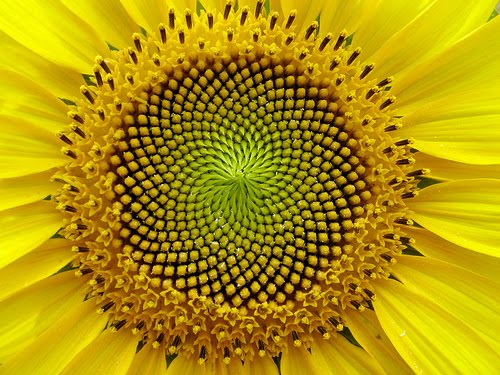
\includegraphics[width=.5\textwidth]{figures/sunflower-seeds}
  \caption{Spiralförmige Anordnung der Röhrenblüten einer Sonnenblume \cite{blender2017howto}}
  \label{fig:sunflower-seeds}
\end{figure}

\subsubsection*{Der Goldene Winkel}
Ausgehend von dem Mittelpunkt der Sonnenblume ist jede nachfolgender Röhrenblüte um rund \ang{137.5} um den Mittelpunkt rotiert. Dieser sogenannte \textit{Goldener Winkel} entsteht durch die Teilung des Vollkreises durch den \textit{Goldenen Schnitt}. Der goldene Schnitt ist ein Teilungsverhältnis das oft bei Größenverhältnissen von einfachen geometrischen Figuren vorkommt und ist wie folgt definiert \cite{wolfram2017golden}:

\begin{equation}
  \Phi = \frac{a}{b} = \frac{a + b}{a} = \frac{1 + \sqrt{5}}{2} \approx 1.618
\end{equation}

Wird der Vollwinkel durch den Goldenen Schnitt geteilt, entsteht der Winkel

\begin{equation}
  \frac{2\pi}{\Phi} \approx \ang{222.5} \,.
\end{equation}

Die Ergänzung zum Vollwinkel ist der Goldene Winkel
\begin{equation}
  2\pi - \frac{2\pi}{\Phi} = \frac{2\pi}{\Phi^2} \approx \ang{137.5} \,.
\end{equation}

Dieser hat die Eigenschaft, dass er aufaddiert nie den selben Winkel ergibt. Diese Eigenschaft machen sich viele Pflanzen zunutze und kann auch in CodeLeaves Anwendung finden.

\subsubsection*{Berechnungen für das Hinzufügen eines Blattes}
Mit dem Vielfachen des goldenen Winkels ist der Winkel $\varphi$ gegeben, um den eine neue Kante eines neuen Blattes um die Senkrechte rotiert werden muss. Für die Position eines neuen Blattes sind aber noch andere Größen zu berechnen.

Angenommen eine Kante mit der endgültigen Länge $l$ wird an einen Knoten K angefügt, um die x-Achse mit dem Winkel $\theta$ geneigt und anschließend um die y-Achse mit den Winkel $\varphi$ rotiert, entsteht ein \textit{Kugelkoordinatensystem} mit der Position von K als Ursprung, der y-Achse als Polachse, der Position des $n$-ten Kindknoten als Punkt $P$, dem \emph{Polarwinkel} $\theta$ und dem \emph{Azimutwinkel} $\varphi$ \cite{papula2001mathematik}.

\begin{figure}[htb]
  \tdplotsetmaincoords{60}{110}
%
\pgfmathsetmacro{\rvec}{1}
\pgfmathsetmacro{\thetavec}{30}
\pgfmathsetmacro{\phivec}{60}
%
\begin{tikzpicture}[scale=7,tdplot_main_coords]

\coordinate (O) at (0,0,0);
\draw[dashdotted,->] (0,0,0) -- (1,0,0) node[anchor=north east]{$z$};
\draw[dashdotted,->] (0,0,0) -- (0,1,0) node[anchor=north west]{$x$};
\draw[dashdotted,->] (0,0,0) -- (0,0,1) node[anchor=south]{$y$};

\tdplotsetcoord{P}{\rvec}{\thetavec}{\phivec}
\coordinate (E) at (Pz);

\draw[thick] (O) node[point,label=above left:$O$]{} -- node[left=3pt]{$h$} (E) node[point,label=above left:$E$]{};
\draw[thick] (O) -- node[below right]{$l$} (P) node[point,label=above right:$P$]{};
\draw (E) -- node[above right]{$a_n$} (P);
\draw[dashed] (O) -- (Pxy);
\draw[dashed] (P) -- (Pxy);
%\draw[dashed] (P) -- (Pyz);
%\draw[dashed] (E) -- (Pyz);

\tdplotsetthetaplanecoords{\phivec}
\tdplotdrawarc[tdplot_rotated_coords]{(E)}{0.1}{90}%
    {180}{above left}{$\cdot$}
\tdplotdrawarc{(O)}{0.2}{0}{\phivec}{anchor=north}{$\varphi$}
\tdplotdrawarc[tdplot_rotated_coords]{(0,0,0)}{0.3}{0}%
    {\thetavec}{anchor=south west}{$\theta$}
    
\end{tikzpicture}

%%Angle Definitions
%%-----------------
%
%%set the plot display orientation
%%synatax: \tdplotsetdisplay{\theta_d}{\phi_d}
%\tdplotsetmaincoords{0}{0}
%
%%define polar coordinates for some vector
%\pgfmathsetmacro{\rvec}{.8}
%\pgfmathsetmacro{\thetavec}{30}
%\pgfmathsetmacro{\phivec}{60}
%
%%start tikz picture, and use the tdplot_main_coords style to implement the display 
%%coordinate transformation provided by 3dplot
%\begin{tikzpicture}[scale=5, tdplot_main_coords]
%
%%set up some coordinates 
%%-----------------------
%\coordinate (O) at (0,0,0);
%
%%determine a coordinate (P) using (r,\theta,\phi) coordinates.  This command
%%also determines (Pxy), (Pxz), and (Pyz): the xy-, xz-, and yz-projections
%%of the point (P).
%%syntax: \tdplotsetcoord{Coordinate name without parentheses}{r}{\theta}{\phi}
%\tdplotsetcoord{P}{\rvec}{\thetavec}{\phivec}
%
%%draw figure contents
%%--------------------
%
%%draw the main coordinate system axes
%\draw[thick,->] (0,0,0) -- (1,0,0) node[anchor=north east]{$x$};
%\draw[thick,->] (0,0,0) -- (0,1,0) node[anchor=north west]{$y$};
%\draw[thick,->] (0,0,0) -- (0,0,1) node[anchor=south]{$z$};
%
%%draw a vector from origin to point (P) 
%\draw[-stealth,color=red] (O) -- (P);
%
%%draw projection on xy plane, and a connecting line
%\draw[dashed, color=red] (O) -- (Pxy);
%\draw[dashed, color=red] (P) -- (Pxy);
%
%%draw the angle \phi, and label it
%%syntax: \tdplotdrawarc[coordinate frame, draw options]{center point}{r}{angle}{label options}{label}
%\tdplotdrawarc{(O)}{0.2}{0}{\phivec}{anchor=north}{$\phi$}
%
%
%%set the rotated coordinate system so the x'-y' plane lies within the
%%"theta plane" of the main coordinate system
%%syntax: \tdplotsetthetaplanecoords{\phi}
%\tdplotsetthetaplanecoords{\phivec}
%
%%draw theta arc and label, using rotated coordinate system
%\tdplotdrawarc[tdplot_rotated_coords]{(0,0,0)}{0.5}{0}{\thetavec}{anchor=south west}{$\theta$}
%
%%draw some dashed arcs, demonstrating direct arc drawing
%\draw[dashed,tdplot_rotated_coords] (\rvec,0,0) arc (0:90:\rvec);
%\draw[dashed] (\rvec,0,0) arc (0:90:\rvec);

%set the rotated coordinate definition within display using a translation
%coordinate and Euler angles in the "z(\alpha)y(\beta)z(\gamma)" euler rotation convention
%syntax: \tdplotsetrotatedcoords{\alpha}{\beta}{\gamma}
%\tdplotsetrotatedcoords{\phivec}{\thetavec}{0}

%translate the rotated coordinate system
%syntax: \tdplotsetrotatedcoordsorigin{point}
%\tdplotsetrotatedcoordsorigin{(P)}

%use the tdplot_rotated_coords style to work in the rotated, translated coordinate frame
%\draw[thick,tdplot_rotated_coords,->] (0,0,0) -- (.5,0,0) node[anchor=north west]{$x'$};
%\draw[thick,tdplot_rotated_coords,->] (0,0,0) -- (0,.5,0) node[anchor=west]{$y'$};
%\draw[thick,tdplot_rotated_coords,->] (0,0,0) -- (0,0,.5) node[anchor=south]{$z'$};

%WARNING:  coordinates defined by the \coordinate command (eg. (O), (P), etc.)
%cannot be used in rotated coordinate frames.  Use only literal coordinates.  

%draw some vector, and its projection, in the rotated coordinate frame
%\draw[-stealth,color=blue,tdplot_rotated_coords] (0,0,0) -- (.2,.2,.2);
%\draw[dashed,color=blue,tdplot_rotated_coords] (0,0,0) -- (.2,.2,0);
%\draw[dashed,color=blue,tdplot_rotated_coords] (.2,.2,0) -- (.2,.2,.2);

%show its phi arc and label
%\tdplotdrawarc[tdplot_rotated_coords,color=blue]{(0,0,0)}{0.2}{0}{45}{anchor=north west,color=black}{$\phi'$}

%change the rotated coordinate frame so that it lies in its theta plane.
%Note that this overwrites the original rotated coordinate frame
%syntax: \tdplotsetrotatedthetaplanecoords{\phi'}
%\tdplotsetrotatedthetaplanecoords{45}

%draw theta arc and label
%\tdplotdrawarc[tdplot_rotated_coords,color=blue]{(0,0,0)}{0.2}{0}{55}{anchor=south west,color=black}{$\theta'$}

%\end{tikzpicture}

%\end{document}
  \caption{Kugelkoordinatensystem mit den zu berechnenden Größen für das Hinzufügen eines neuen Blattes}
  \label{fig:spherical-coordinates}
\end{figure}

Diese Größen sind in Abbildung \ref{fig:spherical-coordinates} dargestellt, wobei die Höhe $h$ als Standardhöhe einer Kante gegeben gilt und $E$ mit $(0, h, 0)$ die Position des $0$-ten Kindes ist. Die y-Achse wird in Anlehnung an Unity in dieser Arbeit als Senkrechte verwendet. Der Waldboden liegt demnach in einer xz-Ebene.

Der Abstand $a_n$ zwischen dem Punkt $E$ und $P$ berechnet sich für den $n$-ten Knoten nach \cite{vogel1979better} mit

\begin{equation}
\label{eq:r}
  a_n = c \sqrt{n} \,,
\end{equation}

wobei $c$ eine Konstante ist und den Abstand der Kindknoten untereinander beeinflusst.

Die Rotation um die y-Achse $\varphi$ ist wie oben hergeleitet das $n$-te Vielfache vom Goldenen Winkel:

\begin{equation}
  \varphi = \frac{2\pi \cdot n}{\Phi^{2}}
\end{equation}

Der Polwinkel $\theta$ lässt sich mithilfe von $h$ und $r$ berechnen:

\begin{equation}
  \theta = \tan^{-1} \left(\frac{r}{h}\right)
\end{equation}

Die Länge $l$ der Kante kann mit

\begin{equation}
  l = h \cdot \cos\left(\theta\right)
\end{equation}

berechnet werden.

Für die Positionierung des Kindknotens muss der Punkt $P$ vom konstruierten Kugelkoordinatensystem in das kartesische Koordinatensystem umgerechnet werden. Dies wird durch die Formel

\begin{equation}
  \vv{P} =
  \begin{pmatrix}
    \sin\left(\varphi\right) \cdot \sin\left(\theta\right) \cdot l\\
    \cos\left(\theta\right) \cdot l\\
    \cos\left(\varphi\right) \cdot \sin\left(\theta\right) \cdot l
  \end{pmatrix}
\end{equation}

erreicht \cite{wolfram2017spherical}.

Damit ist alles für den Algorithmus gegeben, der Blätter eines Knotens mit gleichmäßigem Abstand auf eine gegebene Höhe verteilt und die Kanten entsprechend rotieren und skalieren kann.

In Unity und C\# ist dieser Algorithmus in vereinfachter Form in Listing \ref{lst:addnode} zu sehen ist.

\begin{codesnippet}{Hinzufügen von Blättern eines Knotens}{lst:addnode}
for (var i = 0; i < node.Children.Count; i++)
{
    var d = TreeGeometry.CalcDistance(i);
    var phi = TreeGeometry.CalcPhi(i);
    var theta = TreeGeometry.CalcTheta(DefaultEdgeHeight, r);
    var l = TreeGeometry.CalcEdgeLength(DefaultEdgeHeight, theta);
    var pVec = TreeGeometry.CalcNodePosition(l, theta, phi);

    AddEdgeObject(l, theta, phi);
    AddEmptyNodeObject(pVec);
}
\end{codesnippet}

Das Ergebnis ist in Abbildung \ref{fig:sunflower-algorithm} zu sehen. Auf der linken Seite (\ref{fig:sunflower-30}) sind 30 Blätter verteilt worden. Die Ähnlichkeit zur Verteilung der Röhrenblüten der Sonnenblume wird auf der rechen Seite (\ref{fig:sunflower-200}) mit der Extremsituation mit 200 Blättern und kleiner Konstante $c$ sichtbar. Darin wurde um die Blätter ein Umrandung hinzugefügt, um die Blätter voneinander abgrenzen zu können.

\setlength{\fwidth}{.49\textwidth}
\begin{figure}[htb]
  \centering
  \begin{subfigure}[b]{\fwidth}
   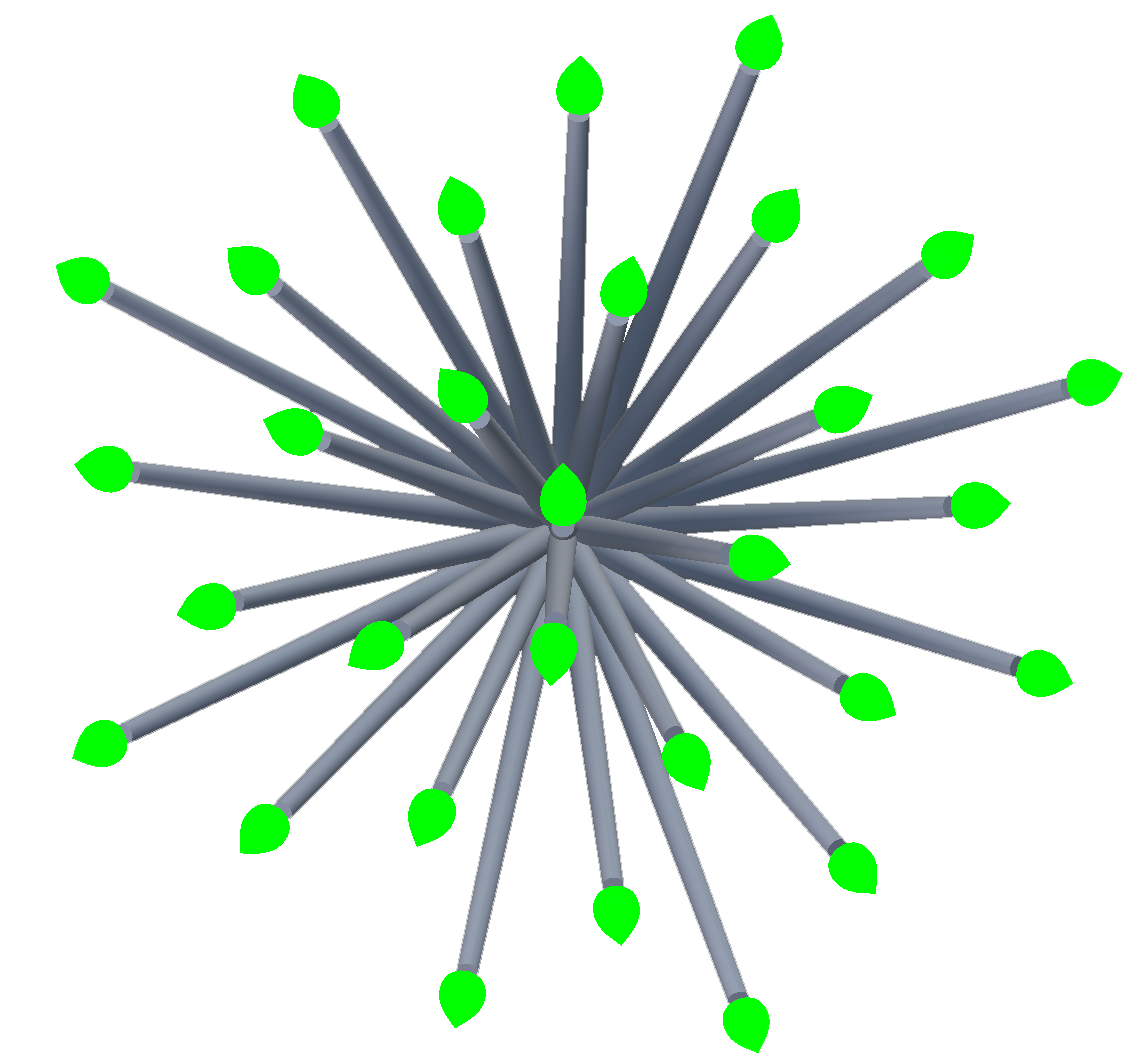
\includegraphics[width=\textwidth]{figures/sunflower-30_2}
   \subcaption{30 Blätter mit $c = 0.05$} \label{fig:sunflower-30}
  \end{subfigure}
  \hfill
  \begin{subfigure}[b]{\fwidth}
  	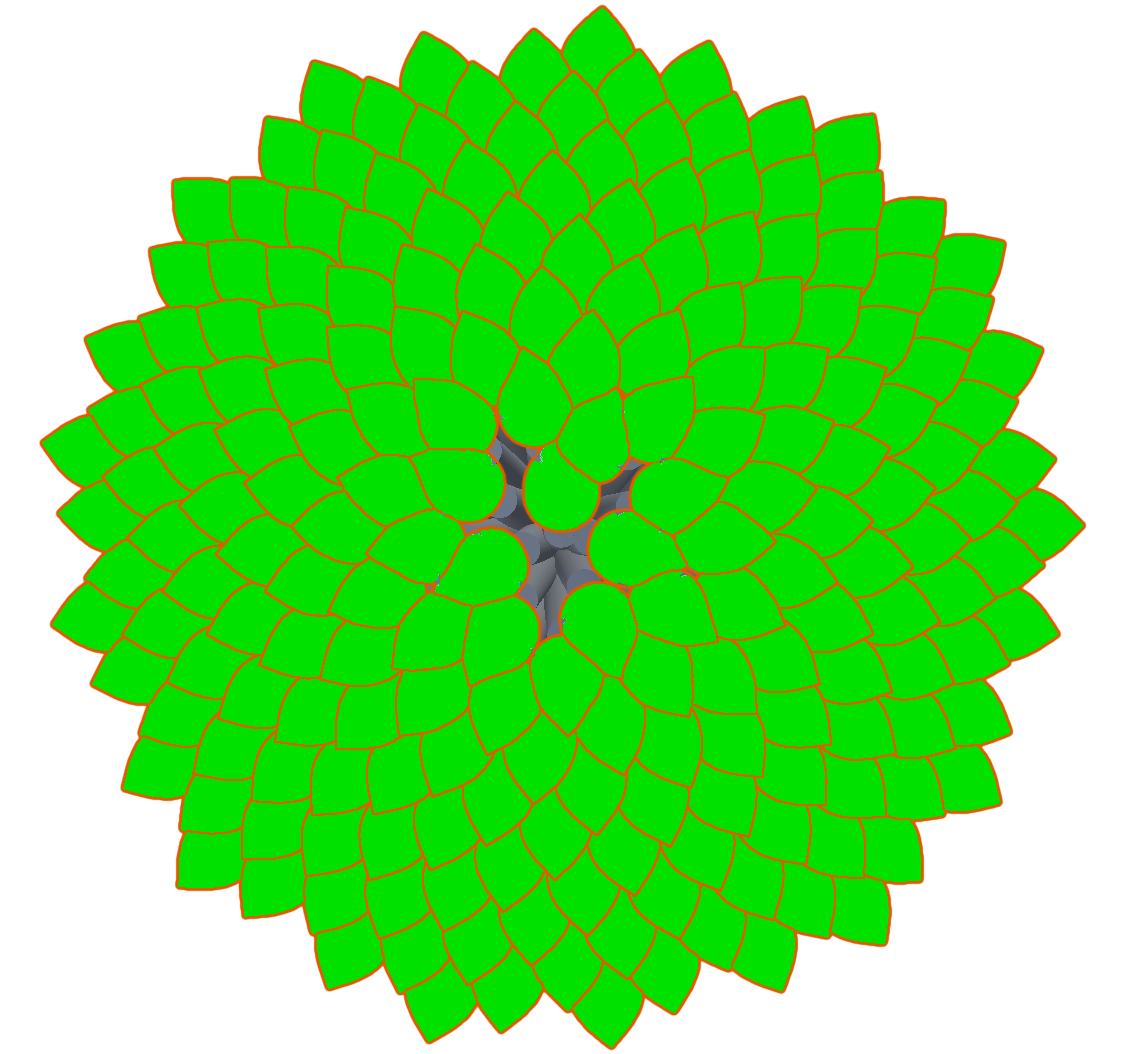
\includegraphics[width=\textwidth]{figures/sunflower-200}
  	\subcaption{200 Blätter mit $c = 0.01$} \label{fig:sunflower-200}
  \end{subfigure}
  \caption{Sonnenblumen-Algorithmus zur Verteilung von Blättern} \label{fig:sunflower-algorithm}
\end{figure}

\section{Verteilung innerer Knoten mit Circle-Packing}
\label{sec:Circle-Packing}

Die Verteilung mit dem Sonnenblumen-Algorithmus beruht auf der Tatsache, dass die Kinder des Knotens mit gleichmäßigem Abstand zueinander verteilt werden können. Dies ist bei inneren Knoten, die wiederum innere Knoten als Kinder besitzen, nicht gegeben. In diesem Fall muss die Breite der Kinder mit berücksichtigt werden, sodass die Äste der einzelnen Kinder nicht kollidieren.

Für die Verteilung der inneren Knoten führen wir ein weiteres Merkmal ein.

\begin{defbox}{Kreis eines inneren Knotens}{radius}
   Der Kreis eines inneren Knotens ist der Kreis, aus dem alle Nachfahren des Knotens von oben betrachtet nicht hinaus ragen.
\end{defbox}

Bei einem inneren Knoten, dessen $N$ Kinder nach dem Sonnenblumen-Algorithmus verteilt wurden, kann der Radius seines Kreises leicht berechnet werden. Der Radius $r$ ist gleich dem Abstand $a_N$ des $N$-ten Blattes, der nach Formel \ref{eq:r} mit $a_N = c \sqrt{N}$ berechnet werden kann.

Werden nun alle inneren Knoten so verteilt, dass sich von oben betrachtet die Kreise der Kinder nicht überschneiden, sind alle Äste eines Baumes kollisionsfrei verteilt und alle Blätter sind von oben sichtbar.

Das Problem der Verteilung von inneren Knoten kann demnach auf jeder Ebene eines Baumes auf 2D reduziert werden.\\

\textit{Es wird ein Algorithmus gesucht, der Kreise unterschiedlicher Größe auf möglichst kleinem Raum überschneidungsfrei positioniert.}\\

Diese Aufgabenstellung wird vom sogenannten \textit{Circle-Packing} gelöst.

Dazu hat W.\ Wang in \cite{wang2006visualization} 2006 einen Algorithmus entworfen, der seitdem von vielen adaptiert worden ist. Zum Beispiel verwendet M.\ Bostock, der Schöpfer in der populären JavaScript Library \textit{d3.js} zur Datenvisualisierung, diesen Circle-Packing-Algorithmus in d3.js \cite{bostock2017abetter}. In 3D wurde er jedoch noch nicht angewandt.

Der Algorithmus muss noch an die Gegebenheiten von CodeLeaves angepasst werden. Bei Wang's Version startet der Algorithmus bereits mit drei tangentialen Kreisen. Der Mittelpunkt, um den zusätzliche Kreise positioniert werden, befindet sich zwischen den drei initialen Kreisen. Bei CodeLeaves sind aber nicht zwangsläufig bei jedem Knoten mindestens drei Kindknoten zu verteilen und als Mittelpunkt für die Verteilung der Kreise ist der Mittelpunkt des $0$-ten Kreises sinnvoll, da sich so immer eine Verlängerung des Stammes ergibt.

Ist nur ein Knoten zu verteilen, wird der Mittelpunkt seines Kreises von oben gesehen (in der xz-Ebene) in den Ursprung gelegt. Der Kreis eines zweiten Knotens wird in einem zufälligen Winkel tangential zum Kreis des ersten Knotens positioniert. Bereits bei einem dritten Kreis kann Wangs's Algorithmus Anwendung finden.

Es wird eine sogenannte \textit{Front-Chain} verwendet, eine zyklische Liste, die alle Kreise enthält, an die potentiell ein neuer Kreis angefügt werden könnte. Die Front-Chain ist in Abbildung \ref{fig:circle-packing} als dickere Linie dargestellt. Bei der Positionierung des ersten bzw.\ des zweiten Kreises werden diese zur Front-Chain hinzugefügt.

Im Ganzen ist der leicht modifizierte Algorithmus für eine Menge von Kreisen $\lbrace C_i \mid i = 0, 2 \cdots N \rbrace$ im Folgenden beschrieben:

\subsubsection*{Abgewandelte Form von Wang's Circle-Packing-Algorithmus (nach \cite{wang2006visualization})}

\begin{enumerate}[(i), labelindent=0pt, align=left, itemsep=0pt, parsep=0pt, labelsep=.5em, leftmargin=!]
  \item Falls $i = 0$ setzte den Mittelpunkt von $C_0$ in den Ursprung und füge $C_0$ zur Front-Chain hinzu.
  \item Falls $i = 1$ setzte den Mittelpunkt von $C_1$ so, dass $C_1$ in einem zufälligen Winkel tangential zu $C_0$ ist und füge $C_1$ zur Front-Chain hinzu.
  \item Für $1 < i < N$ suche $C_m$, der Kreis dessen Mittelpunkt am nächsten zum Ursprung liegt. $C_n$ ist der Kreis in der Front-Chain nach $C_m$ ($n=m+1$).
  \item Berechne den Mittelpunkt von $C_i$ so, dass er tangential zu $C_m$ und $C_n$ ist.
  \item Suche einen Kreis $C_j$ der sich mit $C_i$ überschneidet.
  \item Falls der $C_j$ nicht existiert, setze $C_i$ gleich $C_{i+1}$ und gehe zu (iii).
  \item Falls $C_j$ in der Front-Chain näher an $C_m$ als an $C_n$ liegt, lösche alle Kreise aus der Front-Chain, die zwischen $C_j$ und $C_n$ liegen. Setze $C_m$ gleich $C_j$ und gehe zu (iv).
  \item Falls $C_j$ in der Front-Chain näher an $C_n$ als an $C_m$ liegt, lösche alle Kreise aus der Front-Chain, die zwischen $C_m$ und $C_j$ liegen. Setze $C_n$ gleich $C_j$ und gehe zu (iv).
\end{enumerate}

\label{subsec:collision}\setlength{\fwidth}{.4\textwidth}
\begin{figure}[htb]
  \captionsetup{justification=centering}
  \begin{subfigure}[t]{\fwidth}
   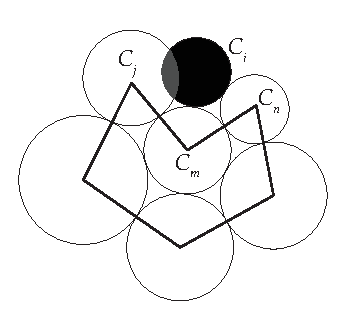
\includegraphics[width=150px]{figures/add-circle}
   \subcaption{Platzieren eines neuen Kreises} \label{fig:add-circle}
  \end{subfigure}
  \hspace{1cm}
  \begin{subfigure}[t]{\fwidth}
  	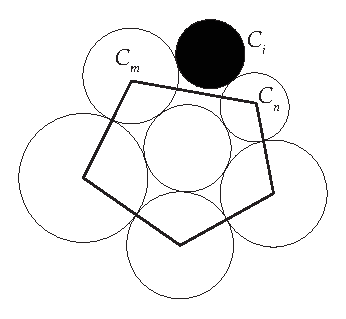
\includegraphics[width=150px]{figures/update-frontchain}
  	\subcaption{Anpassung der Front-Chain und erneutes Platzieren} \label{fig:update-frontchain}
  \end{subfigure}
  \caption{Wang's Circle Packing Algorithmus (nach \cite{bostock2017abetter})}
  \label{fig:circle-packing}
\end{figure}

In Abbildung \ref{fig:Circle-Packing} ist ein Ausschnitt aus dem Algorithmus visualisiert. Auf der linken Seite (\ref{fig:add-circle}) ist Schritt (iv) dargestellt, wobei $C_j$ existiert und und näher an $C_m$, als an $C_n$ liegt. Demnach werden alle Knoten zwischen $C_j$ und $C_n$ aus der Front-Chain entfernt (im Beispiel nur $C_m$) und $C_i$ wird erneut platziert. Das Resultat ist auf der rechten Seite (\ref{fig:update-frontchain}) zu sehen.

Werden die Knoten vor der Durchführung des Algorithmus nach deren Radien sortiert, befindet sich der Knoten mit dem größten Kreis genau über dem Stamm und nach außen hin werden die Äste kleiner, was einem natürlichem Wuchs am nächsten kommt. Durch die zufällige Positionierung des $1$-ten Knotens, wächst der Baum nicht bei jedem Knoten "`in die gleiche Richtung"' was das natürliche Bild des Waldes ebenfalls fördert.

Der oben beschriebene Algorithmus setzt in (ii) und in (iv) die Berechnung eines Mittelpunktes voraus, sodass dessen Kreis tangential zu einem bzw.\ zwei weiteren Kreisen ist.

Bei dem $1$-ten Kreis mit Radius $r_1$ und Mittelpunkt $M_1$, der nur tangential zu dem $0$-ten Kreis mit $r_0$ und $M_0 = (0,0)$ ist und mit dem zufälligen Winkel $\alpha$ platziert wird, ergibt sich für die xz-Ebene folgende Koordinate:

\begin{equation}
  \vv{M}_1 =
  \begin{pmatrix}
    x = \cos\left(\alpha\right) \cdot \left(r_1 + r_2\right)\\
    y = \sin\left(\alpha\right) \cdot \left(r_1 + r_2\right)\\
  \end{pmatrix}
\end{equation}

Bei allen weitern Kreisen $C_i$ ist die Berechnung komplexer. Der Sachverhalt ist in Abbildung \ref{fig:tangent-circle} abgebildet. Gesucht ist $M_3$. Gegeben sind die Mittelpunkte $M_1$ und $M_2$ sowie die Radien der drei Kreise.

\begin{figure}[htb]
  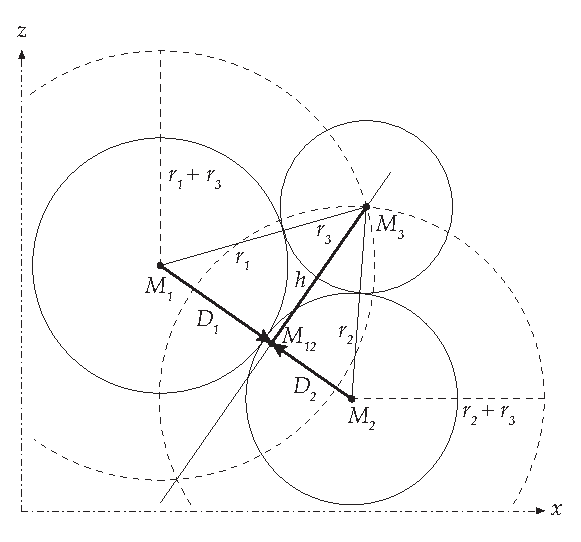
\includegraphics[width=261.593px]{figures/tangent-circle}
  \caption{Berechnung des Mittelpunktes eines Kreises, tangential zu zwei anderen Kreisen}
  \label{fig:tangent-circle}
\end{figure}

$M_3$ befindet sich genau an einem Schnittpunkt der beiden Kreise $\lbrace X \in XZ \mid \overline{M_1 X} = r_1 + r_3 \rbrace$ und $\lbrace X \in XZ \mid \overline{M_2 X} = r_2 + r_3 \rbrace$, die in Abbildung \ref{fig:tangent-circle} gestrichelt veranschaulicht sind. Diese Schnittpunkte lassen sich mithilfe von Vektorrechnung nach \cite{wikipedia2017schnitt} wie folgt errechnen:

\begin{equation}
  \vv{M}_{3_{1/2}} = \vv{M}_1 + \vv{D}_{1} \pm h \cdot \vv{e}
\end{equation}

Dabei ist $e$ ein zu $M_2 - M_1$ orthogonaler Einheitsvektor, für $h$ gilt

\begin{equation}
\label{equ:h}
  h = \sqrt{r_1^2 - \vert \vv{D_1} \vert^2} = \sqrt{r_2^2 - \vert \vv{D_2} \vert^2}
\end{equation}

und $D_1$ lässt sich durch Umformen der Gleichung \ref{equ:h} mit

\begin{equation}
  \vv{D}_1 = \frac{1}{2} \cdot \left( \frac{r_1^2 - r_2^2}{\vert \vv{M}_2 - \vv{M}_1 \vert} + 1 \right)
\end{equation}

darstellen.

Mit diesen Gleichungen kann der Circle-Packing-Algorithmus für Kinder eines Knotens angewandt werden. Für die Positionierung der Knoten im dreidimensionalen Raum kommt für die y-Koordinate jeweils noch die Länge der Kante des $0$-ten Geschwisters hinzu. Die Kanten der Geschwister müssen entsprechend deren Position angepasst werden

\subsubsection*{Knoten mit gemischten Kindern}

Für den Fall, dass ein Paket innere Knoten \textbf{und} Blätter enthält, kann der Circle-Packing-Algorithmus ebenfalls angewandt werden. Dafür muss lediglich einem Blatt ein Radius zugewiesen werden. Mit der Verwendung der Konstante $c$ aus dem Sonnenblumen-Algorithmus als Radius, haben die Blätter bei beiden Verteilungs-Algorithmen den gleichen Abstand zueinander. Lediglich die Ausbreitung der Blätter um den Ursprung erfolgt weniger natürlich, als beim Sonnenblumen-Algorithmus.

\subsubsection*{Hierarchische Anwendung}

Für die Anwendung auf mehreren Ebenen ist nach der Verteilung von Kindern eines Knotens $K$ auf Ebene $n$ die Berechnung des Kreises von $K$ nötig, dass in Ebene $n - 1$ die Generation von $K$ verteilt werden kann.

Der Kreis von Knoten $K$, mit Mittelpunkt an der Position von $K$, der alle Kreise der Kinder von $K$ umschließt und mindestens zu einem Kreis eines Kindes tangential ist, nennen wird den \textit{größten umschließenden Kreis}. Sein Radius ist der Abstand vom $0$-ten Kind zum $n$-ten Kind, zuzüglich des Radius des $n$-ten Kindes. Diese Methode ist nicht der \textit{kleinste umschließende Kreis}, reicht für die Generierung von überschneidungsfreien Bäume jedoch aus.

Für die vollständige hierarchische Anwendung des Circle-Packing wird für jeden Knoten das Circle-Packing rekursiv durchgeführt und anschließend der Radius des eigenen Kreises gesetzt. Abbruchbedingung für die Rekursion ist, dass der Knoten ein Blatt oder ein innerer Knoten mit ausschließlich Blättern ist. In letzterem Fall greift der Sonnenblumen-Algorithmus.

Das heißt der Algorithmus fängt mit dem Knoten mit der maximalen Tiefe an und arbeitet sich über Geschwister und Elternteile bis hin zum Kronenansatz fort, bis alle Knoten eines Baumes verteilt sind.

\subsubsection*{Verteilung von Bäumen}


Nachdem die Kronenansätze Kreise besitzen, sind damit auch die Radien der ganzen Bäume bekannt. Damit können die Bäume prinzipiell beliebig platziert werden, ohne dass sich deren Äste überschneiden. Es wäre zum Beispiel eine Verteilung in einem Gitter möglich, was dann an eine Baumschule mit Baumreihen erinnern würde. Es ist jedoch auch ganz einfach möglich die Bäume ebenfalls mit Circle-Packing anzuordnen. Damit entsteht ein runder Wald und die Bäume nehmen möglichst wenig Platz ein.

Mit den beiden beschriebenen Algorithmen können Bäume garantiert überschneidungsfrei generiert und verteilt werden. Der damit generierte Wald des Projektes Air ist von der Seite in Abbildung \ref{fig:layout-side} und von oben in \ref{fig:layout-top} zu sehen. Die Kreise in Abbildung \ref{fig:layout-top} sind die Visualisierungen der durch das Circle-Packing entstehenden Kreise. Aus der Vogelperspektive ist gut zu erkennen, wie die Blätter innerhalb ihrer Eltern mithilfe des Sonnenblumen-Algorithmus sehr gleichmäßig verteilt werden. Die Farben der Blätter werden in Abschnitt \ref{sec:data} aufgegriffen.

Auch das Circle-Packing ist durch die Kreise gut zu sehen. Jedoch lässt sich feststellen, dass durch die Wahl des größten umschließenden Kreises Platz "verschenkt" wird. Besonders in der Mitte der Abbildung wird dies durch die große Fläche deutlich, in der keine weiteren Knoten platziert sind.

Um das zu umgehen, müsste anstelle des größten umschließenden Kreises der kleinste umschließende Kreis verwendet werden. Dies ist ein weiteres mathematisches Problem und als Teil des \textit{Appollonius} Problem bekannt \cite{dergiades2007soddy}.

Für den Prototyp ist die Umsetzung des kleinsten umschließenden Kreises für CodeLeaves aber nicht essentiell. Entscheidend ist, dass die Struktur der visualisierten Software ohne Überschneidungen dargestellt wird, was auch mit dem größten umschließenden Kreis möglich ist. Die Umstellung auf den kleinsten umschließenden Kreis ist deshalb eine weiterführende Aufgabe.

\begin{figure}[htbp]
  \centering
  \begin{subfigure}[t]{\textwidth}
    \centering
    \includegraphics[width=\textwidth]{figures/layout}
    \subcaption{Seitenansicht} \label{fig:layout-side}
  \end{subfigure}
  \par\bigskip
  \begin{subfigure}[t]{\textwidth}
    \centering
  	\includegraphics[width=\textwidth]{figures/Circle-Packing}
  	\subcaption{Vogelperspektive mit visualisierten Circle-Packing} \label{fig:layout-top}
  \end{subfigure}
  \caption{Layout des Waldes} \label{fig:layout}
\end{figure}

\section{Verwendete Algorithmen in der Praxis}

Für die Praxis in Unity ist bei der Verteilung der Bäume noch zu beachten, dass deren Radien erst verfügbar sind, nachdem der Circle-Packing-Algorithmus für alle Bäume vollständig durchlaufen wurde. Das heißt, dass bei der Generierung der einzelnen Bäume noch nicht bekannt ist, an welcher Position die Bäume letztendlich gesetzt werden müssen und zunächst zum Beispiel an der gleichen Stelle generiert werden müssen. Das bedeutet wiederum, dass bei nicht blockierendem Rendern und großen Projekten wie Air zunächst die Bäume überlagernd gerendert werden und dies auch durchaus für einige Sekunden für den Nutzer sichtbar ist, bevor sich die Bäume verteilen.

Bei Air dauert die Generierung der 40 Bäume im Unity Editor auf einer Hardware mit 2.3 GHz Intel Core i7 CPU und 16 GB 1600 MHz DDR3 RAM bei 10 Messungen zwischen 6,5 und 6,8 Sekunden. Auf der HoloLens stehen keine genauen Messdaten zur Verfügung, die Generierung dauert aber noch etwas länger.

Soll vermieden werden, dass der Nutzer zunächst die überlagernde Generierung mit ansieht, dürften die Bäume erst sichtbar werden, nachdem alle Bäume fertig generiert und verteilt worden sind.

Ein weiterer zu beachtender Punkt ist die Leistungsfähigkeit der HoloLens. Für Air werden über 12 Tausend 3D Objekte gleichzeitig gerendert. Die aktuelle Entwickler-Version der HoloLens ist für diese Summe an zu rendernden Objekten nicht ausgelegt. Bei Generierung des Waldes wird das Bild zunächst kurz schwarz und stockt während und auch nach fertiger Generierung merklich. Auch bei kontinuierlichen Interaktionen wie das Skalieren reagiert die HoloLens erst nach beendeter Eingabe. Die Nutzung von so großen Software-Projekten wie Air ist demnach mit der aktuellen Entwickler-Version der HoloLens möglich, aber nicht besonders angenehm. Dagegen laufen kleinere Projekte, oder ein Ausschnitt von Air mit z.\,B.\ nur 5 statt den eigentlichen 40 Bäumen flüssig.

\section{Abbildung von Daten auf die Struktur}
\label{sec:data}

In Abbildung \ref{fig:layout} waren bereits unterschiedliche Blattfarben zu sehen. Mit der Generierung des Waldes ist das schwierigste geschafft. Das Färben der Blätter und das Anpassen der Dicke der Kanten und Wurzeln ist dagegen trivial.

\subsubsection*{Farbe der Blätter}

In den Abbildung \ref{fig:layout} - \ref{fig:root} wird mit der Blattfarbe die Testabdeckung im Projekt Air visualisiert. Damit ist es möglich eine beliebige Metrik darzustellen, die im Software-Meta-Modell vorliegt (Akz. \ref{acc:s-metrics} und \ref{acc:d-metrics}). Die Metrik kann in einem stufenlosen Farbverlauf dargestellt werden, im Beispiel der Testabdeckung von Rot (0\%) über Gelb (50\%) bis hin zu Grün (100\%). Klassen, bei denen im Beispiel-Datensatz keine Testabdeckung verfügbar ist, erscheinen in Grau.

In Abbildung \ref{fig:leaf-color} ist schön zu sehen, dass die Testabdeckung im Durchschnitt sehr gut ist, obwohl immer wieder Klassen dabei sind, bei denen die Testabdeckung gering ist. Im linken oberen Eck der Abbildung ist ein Ast zu sehen, bei dem alle Blätter keine gute Testabdeckung vorweisen können. Ausreißer der aktuellen Metrik und ganze Hotspots sind demnach im Prototyp gut zu erkennen (Akz. \ref{acc:s-hotspots} und \ref{acc:d-hotspots}).

\begin{figure}[htb]
  \includegraphics[width=\textwidth]{figures/leaf-color}
  \caption{Farbe der Blätter und Erkennung von Ausreißern}
  \label{fig:leaf-color}
\end{figure}

\subsubsection*{Dicke der Kanten}

Die Dicke der Kanten lässt sich ebenfalls leicht anpassen. Die Standard-Dicke kann je nach Anzahl der direkten Verbindungen mit einer geeigneten mathematischen Funktion erhöht werden. Da der Beispiel-Datensatz von Air jedoch keine Verbindungen wie Abhängigkeiten aufweist, wird in Abbildung \ref{fig:thickness} ein Baum gezeigt, der mit zunehmender Höhe der Knoten entsprechend dickere Kanten besitzt. Dies ist für richtige Verbindungen wie Abhängigkeiten natürlich wenig realistisch, zeigt aber das Potential dieser Darstellung. Die Beschaffung und der Transfer von Daten über Abhängigkeiten in Air in das Software-Meta-Modell ist keine triviale Aufgabe und muss außerhalb dieser Arbeit bewältigt und vor allem auch automatisiert werden.

Akzeptanzkriterium \ref{acc:s-thickness} und \ref{acc:d-thickness} wird demnach im High-Fi Prototyp bereits technisch erfüllt. Es muss aber mit realistischen Beispieldaten noch evaluiert werden, welche mathematische Funktion für die Dick der Kanten geeignet ist.

\begin{figure}[htb]
  \includegraphics[width=\textwidth]{figures/thickness}
  \caption{Unterschiedliche Dicke der Kanten}
  \label{fig:thickness}
\end{figure}

\subsubsection*{Wurzeln}

Bislang haben wir nur Wälder ohne Wurzeln gesehen. Eine realistische Darstellung vom Wurzelgeflecht ist aufgrund der unzureichenden Beispieldaten ebenfalls nicht möglich. Jedoch werden Wurzeln im High-Fi Prototyp prinzipiell  unterstützt. In Abbildung \ref{fig:root} ist eine Beispiel-Wurzel zu sehen, die zwei Bäume miteinander verbindet. Für eine Wurzel wird als 3D Objekt ein Zylinder verwendet, sodass Wurzeln auch von der Seite gut erkennbar sind.

\begin{figure}[htb]
  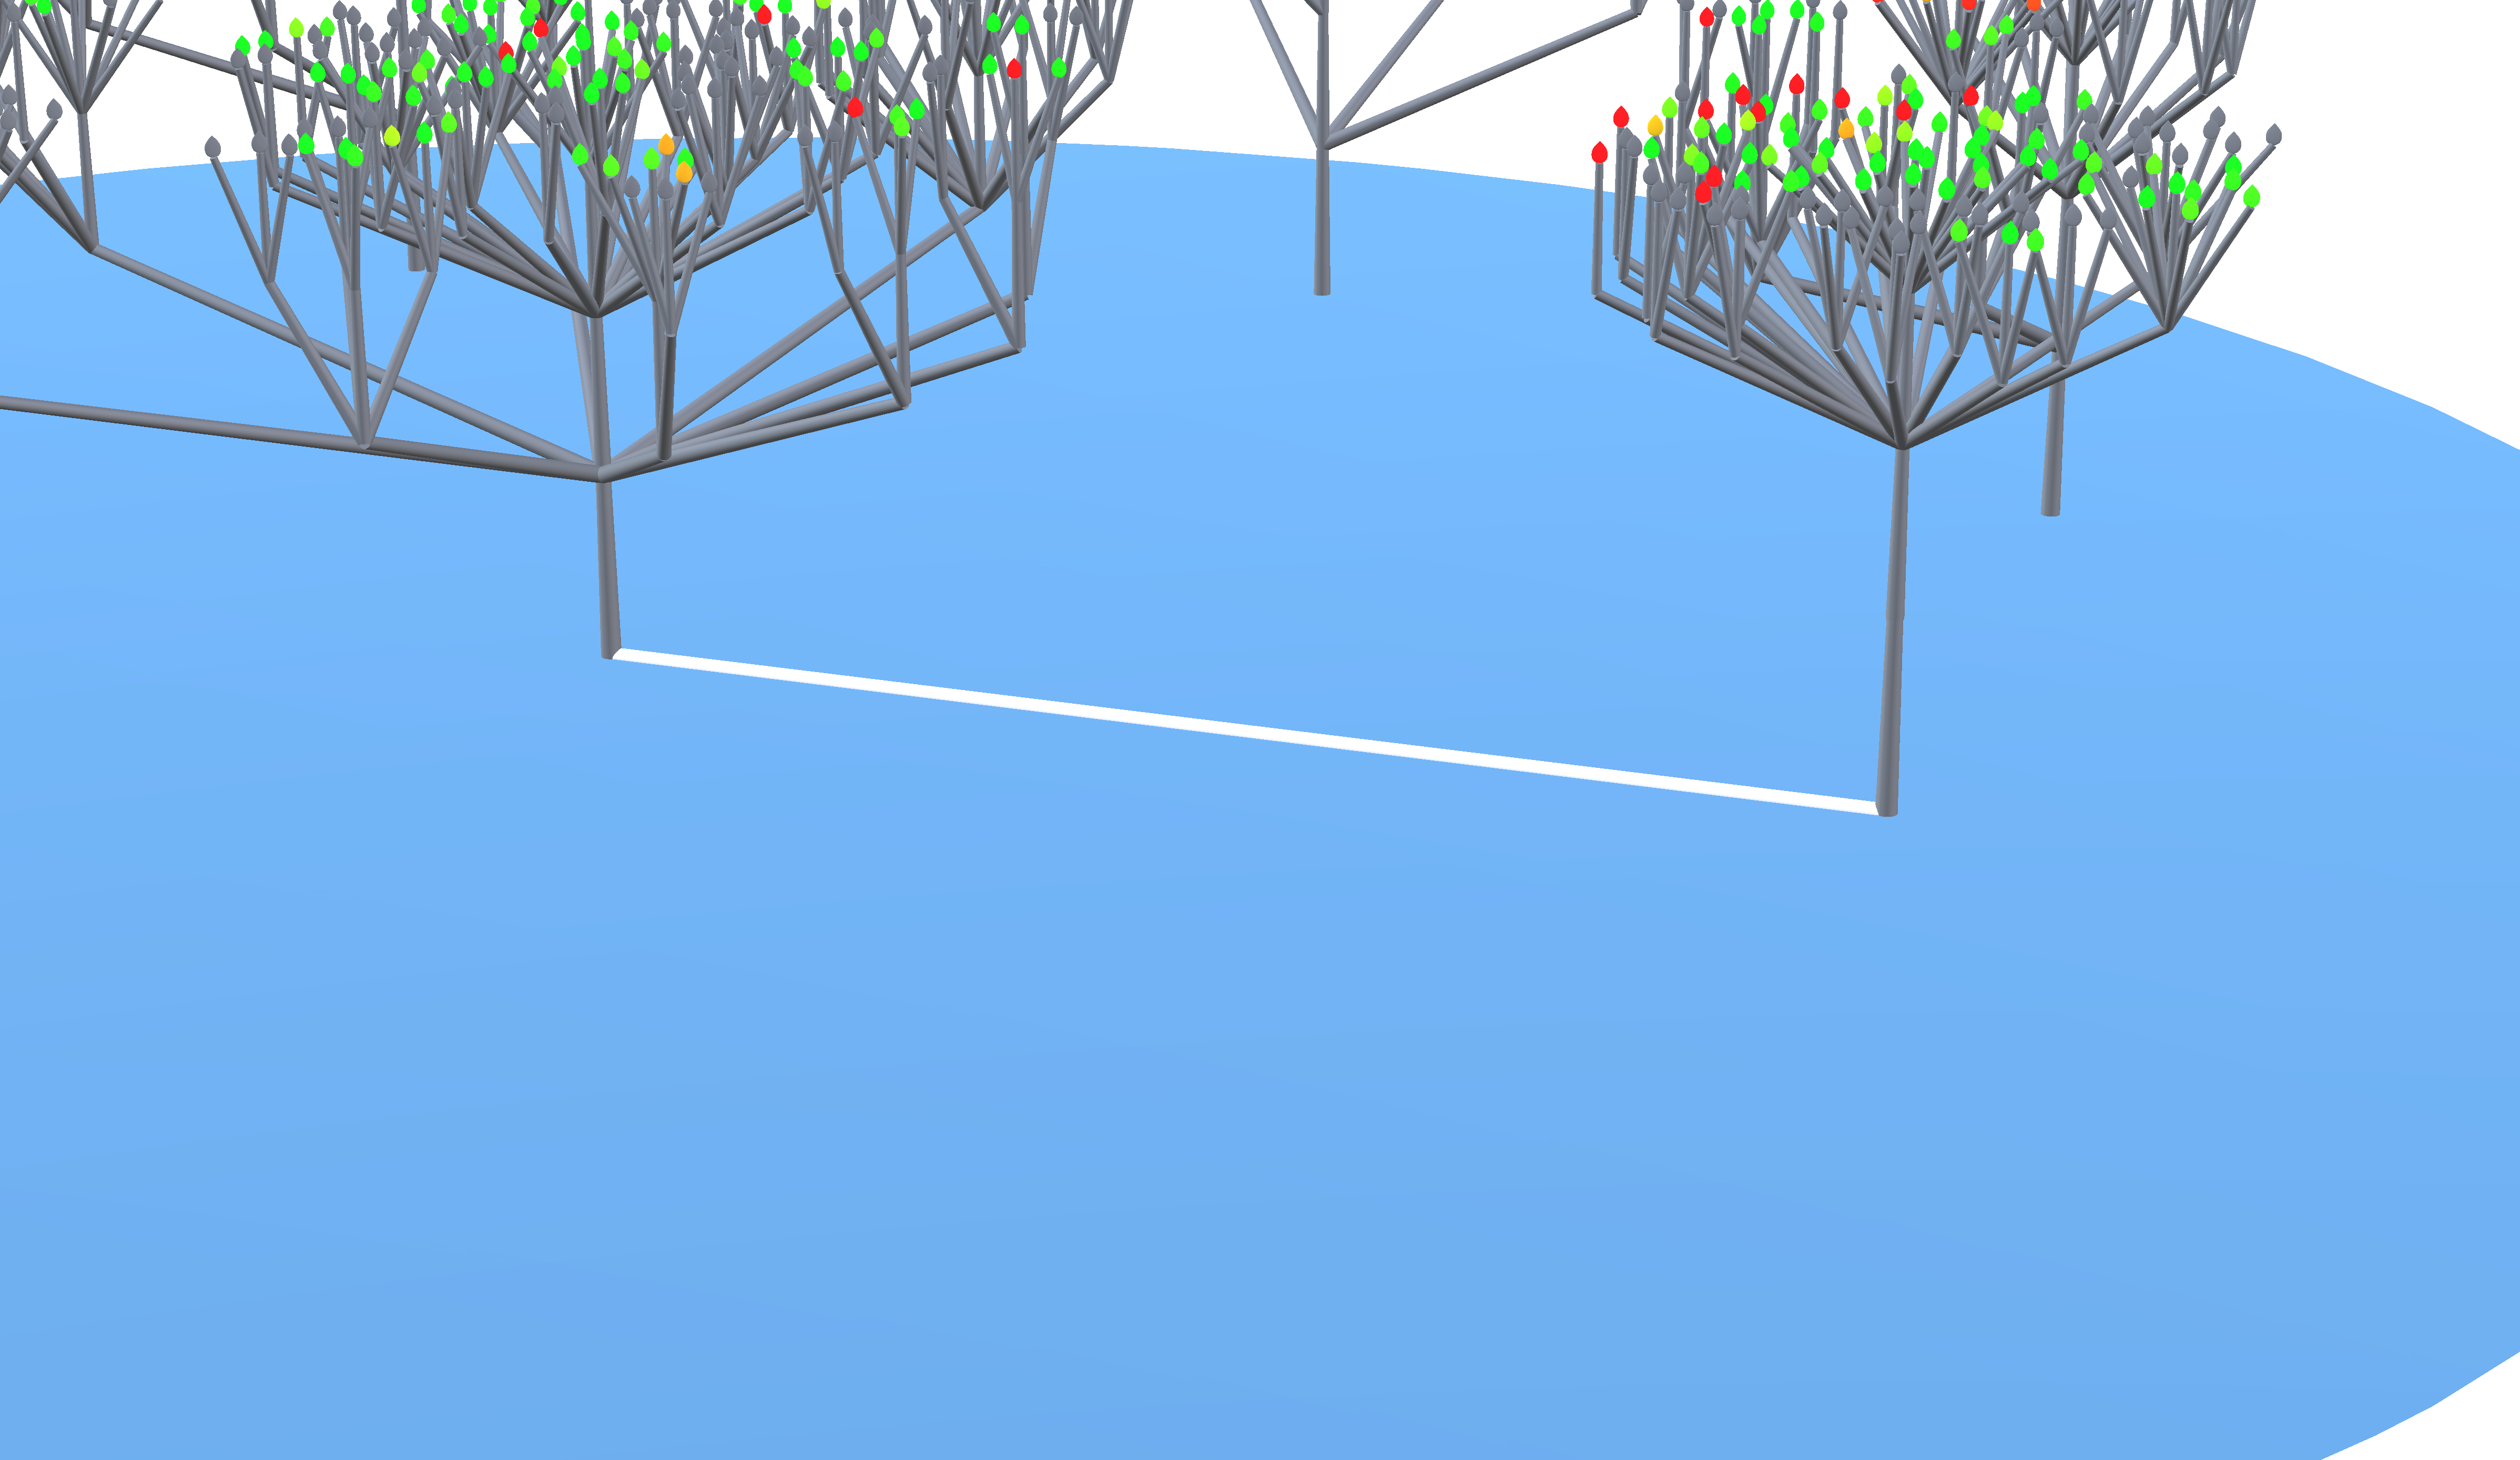
\includegraphics[width=\textwidth]{figures/root}
  \caption{Beispiel einer Wurzel}
  \label{fig:root}
\end{figure}

Die Struktur des Waldes kann nun generiert, die Blätter gefärbt und die Dicke der Kanten und Wurzeln angepasst werden. Was fehlt, ist die Interaktion. Dazu wird im nächsten Kapitel zunächst auf Grundlagen der Interaktion in der AR eingegangen, um diese dann in Kapitel \ref{ch:interaction} bei der Interaktion in CodeLeaves anzuwenden.

% ----==== Chapter ====---- %
\chapter{Grundlagen der Interaktion in der AR}
\label{ch:interaction-ar}

\section{Eingabemöglichkeiten in der AR und mit der HoloLens}
\label{sec:interaction-hololens}

In den frühen 70er-Jahren wurden erste Modelle der Computermaus entwickelt und mit Apple's Lisa aus dem Jahr 1983 wurde sie zum Markterfolg. Heute ist die zeigerbasierte Interaktion mit Computer nicht mehr weg zu denken.

Neben der zeigerbasierten Eingabe hat sich mit dem Einzug von Smartphones und Tablets die auch die touchbasierte Eingabe etabliert. Diese Art der Eingabe kann für Monitor-basierte AR verwendet werden. Ein Beispiel dafür sind iOS Geräte, die Apple's AR-Kit unterstützen.

Für die AR mit \textit{Head-Mounted-Displays} (HMD) Devices, die wie die HoloLens vom Nutzer als Brille getragen werden, ergeben sich neue Möglichkeiten mit Anwendungen zu interagieren. Dies sind folgende:

\begin{enumerate}
  \item Blickrichtung
  \item Gesten
  \item Sprache
  \item Controller
\end{enumerate}

\subsubsection*{Blickrichtung}
Bei der HoloLens ist die \textit{Blickrichtung} (engl.: \textit{Gaze}) ein elementarer Bestandteil der Bedienung der HoloLens \cite{windows2017interaction}. Die Blickrichtung wird im Normalfall mithilfe eines Cursors visualisiert, der der Kopfbewegung des Nutzers folgt und so immer zentral im Sichtfeld der Hololens bleibt. Der Cursor wird so positioniert und orientiert, dass er sich auf der Oberfläche des Objekts befindet, das sich in Blickrichtung befindet und dem Nutzer am nächsten ist. Das Ziel der Blickrichtung nennen wir \textit{fokussiertes} Objekt.

\subsubsection*{Gesten}
Nachdem bei HDM-Devices Hologramme im realen Raum platziert werden, ist Gestensteuerung eine intuitive Eingabemöglichkeit. Beispielsweise muss die Möglichkeit der Auswahl, Platzierung, Skalierung oder Rotation von Hologrammen ermöglicht werden.

Allgemein kann zischen zwei Arten von Gesten unterschieden werden \cite{windows2017gesture}.

\paragraph{Diskrete Gesten} sind solche, in denen die Ausführung der Geste einen binären Status besitzt. D.\,h\ die Ausführung der Geste ist die Information selbst und trägt keine weiteren Informationen. Diese Gesten lassen sich mit einem Klick einer Computermaus vergleichen.

\paragraph{Kontinuierliche Gesten} sind solche, bei denen das Ausmaß der Geste eine Rolle spielt. Das Ausmaß bestimmt die Größe der Eingabe. Vergleichen wir diese Gesten mit einer Computermaus, wäre das die Mausbewegung.\\

Theoretisch sind beliebig viele Gesten denkbar. Zum Beispiel könnte für das Rotieren von Objekten die Rotation einer Hand verwendet werden. Mit Produkten wie zum Beispiel Kinetic\footnote{\url{https://developer.microsoft.com/de-de/windows/kinect}} können solche Gesten auch erkannt werden. Bei der HoloLens sind die unterstützen Gesten jedoch stark begrenzt. Es existieren insgesamt fünf verschiedene Gesten, die von der HoloLens als solche identifiziert werden können. Die sogenannte \textit{Bloom}-Geste ist für das Windows-Menü reserviert. Sie wird ausgeführt, indem der Nutzer alle Fingerspitzen zusammen führt und dann die Hand öffnet und eine aufgehende Blume imitiert.

Als weitere diskrete Geste kann der \textit{Air-Tap} verwendet werden. Dieser ist in Abbildung \ref{fig:Air-Tap} veranschaulicht. In Verbindung mit der Blickrichtung können so Hologramme angeklickt werden.

\begin{figure}[htb]
  \includegraphics[width=.8\textwidth]{\figdir/Air-Tap}
  \caption{Air-Tap \cite{windows2017gesture}}
  \label{fig:Air-Tap}
\end{figure}

Neben dem Air-Tap werden auch der \textit{Double-Tap} und die \textit{Tap-and-hold}-Geste erkannt.

Mit der \textit{Manipulation}-Geste stellt Microsoft eine kontinuierliche Geste zur Verfügung. Wird ein Air-Tap gehalten und die Hand anschließend bewegt, so kann als Eingabe die Positionsänderung der Hand verwendet werden. Damit ist beispielsweise ein Drag-and-Drop von Hologrammen möglich.

Die HoloLens kann zwischen linker und rechtem Hand unterscheiden. Das bedeutet, dass auch eine Interaktion mit der Verwendung von beiden Händen denkbar sind.

\subsubsection*{Sprache}
Neben den Gesten kann auch durch Sprachsteuerung mit Hologrammen interagiert werden. In einer Applikation können beliebige Befehle definiert werden, die dann von der HoloLens automatisch erkannt werden.

Da die Interaktion mit Gesten auf Dauer für die Arme ermüdend sein kann, bietet sich die Sprachsteuerung zur Unterstützung der Gestensteuerung an. Beide Eingabemethoden können auch gut miteinander kombiniert werden. So kann z.\,B. mithilfe von Sprachbefehlen zwischen unterschiedlichen Interaktionsmodi umgeschalten werden. Dadurch können unterschiedliche Interaktionen wie Skalieren und Rotieren mit der gleichen Geste durchgeführt werden.

\subsubsection*{Controller}
Die vierte Möglichkeit der Interaktion mit HMD-Devices sind Controller. Die meisten VR-Headsets sind nur mit solchen Controllern zu bedienen. In der aktuellen Version unterstütz die HoloLens jedoch kein Controller. Bei anderen Windows Mixed Reality Geräten wie die \textit{Immersive} Headsets von Acer und HP\footnote{\url{https://developer.microsoft.com/en-us/windows/mixed-reality/immersive_headset_hardware_details}} können mit den \textit{Motion} Controllern, ähnlich wie bei Gaming Konsolen, mit verschiedenen Tasten unterschiedliche Eingaben getätigt werden. Bei der HoloLens steht lediglich der \textit{Clicker} zur Verfügung, ein kleines Bluetooth-Gerät, das durch physisches Klicken den Air-Tap ersetzen kann. Bei Dauerhafter Eingabe von Air-Tap-Gesten ist der Einsatz vom Clicker angenehm, da man die Hand nicht im Sichtfeld der HoloLens halten muss.

\section{Herausforderungen}

Bei der Entwicklung von AR-Applikationen sind einige Herausforderungen zu beachten, die auch für CodeLeaves von Relevanz sind. Im Zuge der Entwicklung von der HoloLens-Anwendung HoloStudio hat Senior Holographic Designer M.\ Ghaly in \cite{windows2017casestudy3} eine Case Study veröffentlicht. Mitunter traten die im Folgenden betrachteten Herausforderungen auf.

\subsubsection*{Hologramme außerhalb des Sichtfelds}

Da Hologramme im ganzen Raum, in dem sich der Betrachter befindet, platziert werden können, ist nicht immer gewährleistet, dass sie sich auch im Blickfeld des Betrachters befinden. Besonders bei der aktuellen Entwickler-Version der HoloLens ist das Sichtfeld, in dem Hologramme angezeigt werden können, mit rund 30 Grad \cite{czerulla2017microsoft} gering.

Eine Variante dies zu umgehen, ist es \textit{Tag-along}-Objekte zu verwenden. Diese Objekte bleiben immer im Blickfeld des Betrachters. Schaut der Nutzer in eine andere Richtung, wird das Objekt neu positioniert, sodass es wieder ins Blickfeld des Nutzers gelangt. Innerhalb des Blickfelds bleiben Tag-along-Objekte aber stationär, sodass der Nutzer mit der Blickrichtung weiterhin mit ihnen interagieren kann. Das Windows-Startmenü der HoloLens ist ein solches Tag-along-Objekt.

In der Case Study aus \cite{windows2017casestudy3} wurde festgestellt, dass die Probanden sich von solchen Tag-along-Objekten in manchen Fällen bedrängt fühlen und sollten deshalb sparsam verwendet werden.

Eine andere Möglichkeit ist es auf Hologramme, die sich außerhalb des Sichtfelds befinden, gezielt aufmerksam zu machen. Das kann mit verschiedenen Techniken erreicht werden. Eine davon ist die Verwendung von \textit{Spacial-Sound}, was bedeutet, dass Geräusche ebenfalls im Raum platziert werden können und vom Nutzer dreidimensional mit Richtung und Entfernung wahrgenommen werden können. Dies bietet sich vor allem bei Spielen mit bewegten Charakteren an. Bei statischem Content wie CodeLeaves, sind Geräusche nicht besonders intuitiv.

Es kann auch mit zusätzlichen Objekten gearbeitet werden, die dem Nutzer darauf hinweisen, wo seine Aufmerksamkeit erfordert wird. Solche Hilfs-Objekte werden in der HoloLens-Entwicklung \textit{Direction-Indicators}. Diese können unterschiedliche Gestalt annehmen. Bei anderen HoloLens-Applikationen sind Pfeile, Licht oder Denkblasen im Einsatz.

\subsubsection*{UI von anderen Objekten verdeckt}

Ein Problem, das in vielen HoloLens-Applikationen auftritt, ist dass UI-Elemente von anderen Hologrammen, die näher am Nutzer positioniert sind, verdeckt werden können.

Das Problem ist in Abbildung \ref{fig:occlusion} illustriert. Darin wird in CodeLeaves ein Button eines Kontextmenüs (siehe Abschnitt \ref{ch:interaction} von einem Stamm verdeckt.

\begin{figure}[htb]
  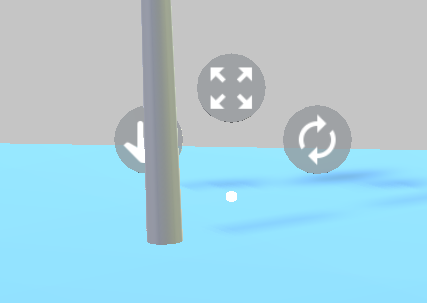
\includegraphics[width=.6\textwidth]{\figdir/occlusion}
  \caption{Verdeckung von UI-Elementen}
  \label{fig:occlusion}
\end{figure}

Analog zum 2D Pop-ups ist es möglich UI-Elemente vor allen anderen Elementen zu platzieren. In 3D bedeutet das, dass das UI-Element vor dem Hologramm erscheinen muss, dass sich am nächsten am Nutzer befindet. Dabei ist zu beachten, dass durch den räumlichen Versatz der Bezug zum fokussierten Objekt nicht verloren gehen darf.

Ein alternativer Lösungsansatz ist der \textit{Shine-through}-Effekt, wie er bei HoloStudio Verwendung findet und in Abbildung \ref{fig:shine-through} veranschaulicht wird. Dabei bleiben UI-Elemente räumlich bei dem fokussiertem Objekt, jedoch scheinen sie durch davor liegende Hologramme durch. Diese Variante ist auch für anzuzeigenden Text gut geeignet.

\begin{figure}[htb]
  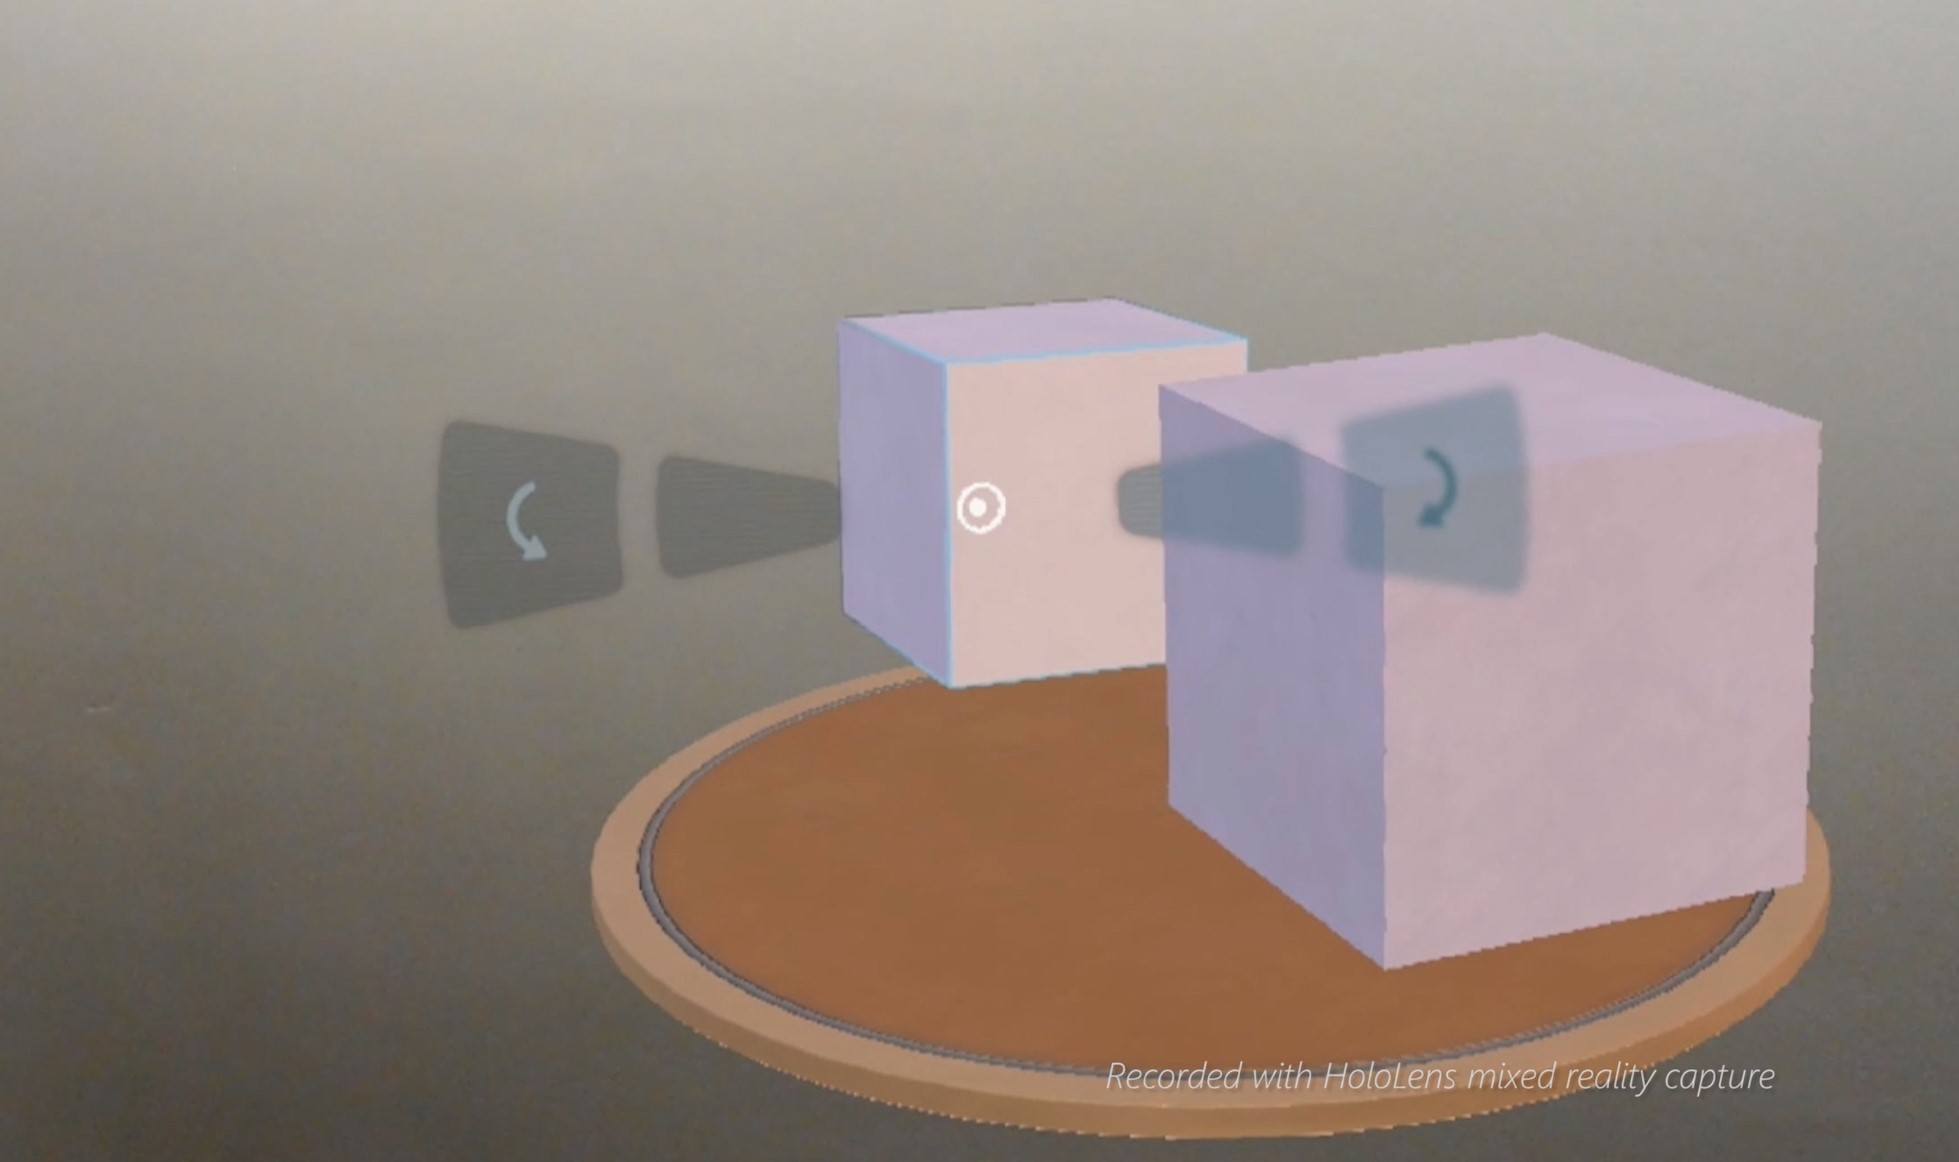
\includegraphics[width=.6\textwidth]{\figdir/shine-through}
  \caption{Shine-through-Effect von UI-Elementen in HoloStudio \cite{windows2017casestudy3}}
  \label{fig:shine-through}
\end{figure}

\section{Technische Umsetzung von Interaktionen mit Reaktiver UI}

\subsubsection*{Motivation}
Eine der offensichtlichen Interaktionen mit CodeLeaves ist das Anklicken von Knoten. Der Nutzer erwartet damit nähere Informationen zu einem Paket oder einer Klasse zu erfahren. Betrachten wir zunächst eine sehr einfaches Szenario:

\begin{quotation}
  \textit{Wenn der Nutzer auf ein Blatt klickt, soll daraufhin der Name der repräsentierten Klasse über dem Blatt erscheinen.}
\end{quotation}

Diese Interaktion ist in Abbildung \ref{fig:leaf-interaction} veranschaulicht.

\setlength{\fwidth}{.49\textwidth}
\begin{figure}[htb]
  \centering
  \begin{subfigure}[b]{\fwidth}
   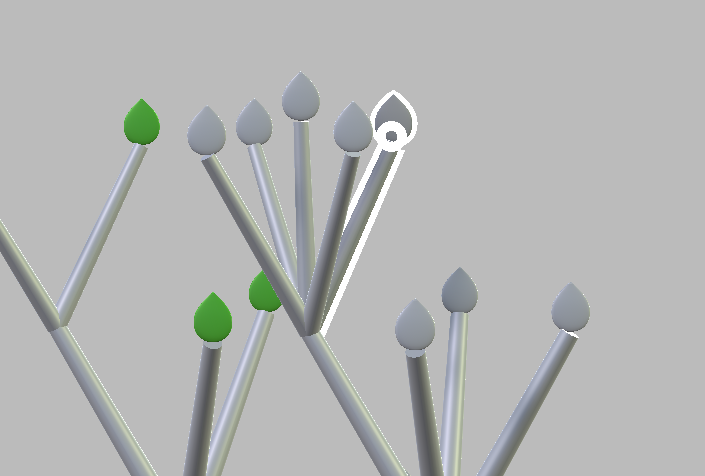
\includegraphics[width=\textwidth]{figures/leaf-focused}
   \subcaption{Fokussiertes Blatt} \label{fig:leaf-focused}
  \end{subfigure}
  \hfill
  \begin{subfigure}[b]{\fwidth}
  	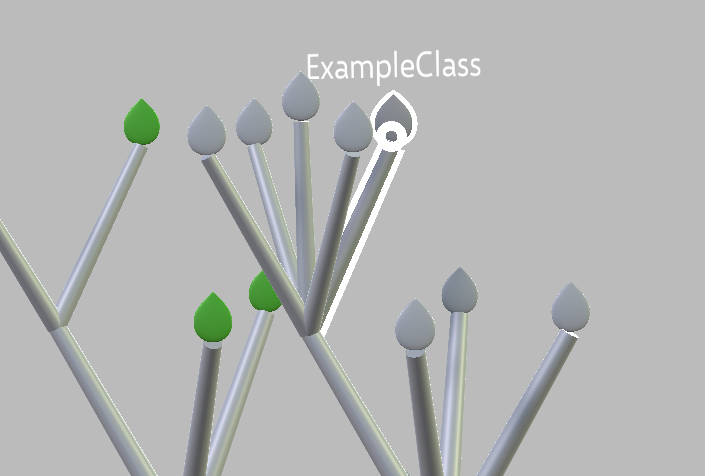
\includegraphics[width=\textwidth]{figures/leaf-clicked}
  	\subcaption{Angeklicktes Blatt} \label{fig:leaf-clicked}
  \end{subfigure}
  \caption{Beispielhafte Interaktion mit einem Blatt} \label{fig:leaf-interaction}
\end{figure}

Bei der Generierung des Baumes wird zu jedem Blatt ein Label hinzugefügt, in dem beliebiger Text gespeichert werden kann. Das Anzeigen des Namens ist demnach kein Problem und könnte wie folgt implementiert werden:

\begin{codesnippet}{Direkte Manipulation (Negativbeispiel)}{lst:direct-manipulation}
public class NodeInputHandler : MonoBehaviour, IInputClickHandler
{
    public void OnInputClicked(InputClickedEventData eventData)
    {
        // Get label of currently clicked node
        var labelObject = GetLabelObject(gameObject);

        // Toggle active
        labelObject.SetActive(!labelObject.activeSelf);
    }
}
\end{codesnippet}

Mit diesem Ansatz könnte also auf das Ereignis des Air-Taps auf einfachste Weise reagiert werden. Wird das Blatt angeklickt, wird das Label-Objekt des Blattes aktiviert und der Name wird damit sichtbar. Entsprechend kann bei erneutem Klick das Label-Objekt wieder deaktiviert werden. Wird die Businesslogik aber komplexer, kommt dieser Ansatz schnell an seine Grenzen.

Eventuell könnte sich zum Beispiel folgende Einstellung in der Applikation als sinnvoll erweisen:

\begin{quotation}
  \textit{Der Nutzer kann einstellen, ob bei einem Klick auf ein Blatt der Klassenname oder die Zahl der gerade visualisierten Metrik angezeigt wird.}
\end{quotation}

Woher weiß die Funktion jetzt was angezeigt werden soll?

Das eigentliche Problem bei der beschriebenen Situation ist, dass Businesslogik und UI eng gekoppelt wurde. Dies sollte tunlichst vermieden werden. Bei einem Klick auf einem Blatt sollte nicht die UI entscheiden was zu tun ist, sondern die Businesslogik. Die Entkopplung von UI und Logik, ist mit reaktiver Programmierung möglich.

Was ist reaktive Programmierung? A.\ Staltz beschreibt es in \cite{staltz2016introduction} als "`Programmierung mit asynchronen Datenströmen."' Dies trifft den Kern. Es geht darum auf Änderungen von Werten zu reagieren, die durch \textit{Streams} propagiert werden.

Streams sind nichts anderes als \textit{Observables}, die bei jeder Änderung ihrer Werte allen registrierten \textit{Subscribers} den neuen Wert mitteilen.

Betrachten wir in Abbildung \ref{fig:label-stream} konkret das Beispiel des Textes, der im Label eines Blattes steht.

\begin{figure}[htb]
  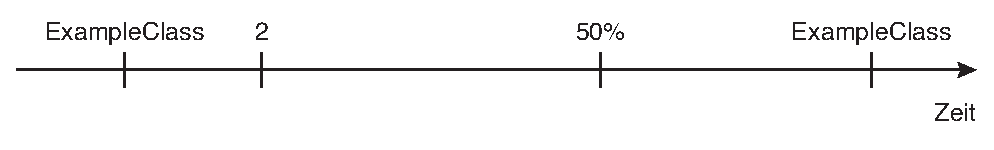
\includegraphics[width=.8\textwidth]{\figdir/label-stream}
  \caption{Datenstrom eines Labels für reaktive Programmierung}
  \label{fig:label-stream}
\end{figure}

Über die Zeit hinweg, kann sich durch die Businesslogik der darzustellende Text verändern. Im Beispiel soll der Klassenname, dann vielleicht Laufzeitfehler, Testabdeckung und dann wieder der Klassenname dargestellt werden.

Bei der Generierung des Baumes muss dann lediglich der Label-Wert observiert und der Text entsprechend gesetzt werden.

\subsubsection*{Verwendung in Unity}

In Unity steht für reaktive Programmierung das Open-Source-Projekt \textit{UniRx}\footnote{\url{https://github.com/neuecc/UniRx}} zur Verfügung, das die Funktionalität der reaktiven .NET Library \textit{Rx} für Unity zugänglich macht. UniRx implementiert z.\,B. \textit{ReactiveProperties}, mit denen eine einfache Verwendung des Observer-Pattern möglich ist. Darüber hinaus bietet die API hilfreiche Stream-Funktionen wie \texttt{filter}, \texttt{map}, \texttt{merge} oder \texttt{join}.

In unserem Beispiel von oben wird der Text eines Blattes des UI-Models zu einer ReactiveProperty und bei jeder Änderung wird der Text des Labels angepasst. Auch das aktivieren des Labels wird über eine ReactiveProperty realisiert. So ist zum Beispiel das deaktivieren von allen Labels gleichzeitig leicht möglich.

In Listing \ref{lst:reactive-property} wird gezeigt, wie eine ReactiveProperty für den Status \texttt{isSelected} eines \textit{UiNodes} definiert wird. Im \texttt{TreeBuilder} (Zeile 9) wird das Label bei Aktualisierung von \texttt{isSelected} entsprechend aktiviert.

\begin{codesnippet}{Observieren von Werten}{lst:reactive-property}
public abstract class UiNode
{
    public ReactiveProperty<bool> isSelected { get; set; }
    ...
}

public class TreeBuilder {
    ...
    node.IsSelected.Subscribe(label.SetActive);
    ...
}

public class NodeInputHandler : MonoBehaviour, IInputClickHandler
{
    public void OnInputClicked(InputClickedEventData eventData)
    {
        InteractionManager.HandleNodeClick(GetNodeId(gameObject));
    }
    ...
}
\end{codesnippet}

Im \texttt{NodeInputHandler} wird nun die Ui nicht mehr direkt manipuliert, sondern es wird eine Funktion des \texttt{InteractionManagers} aufgerufen, die sich darum kümmert, das UI-Model entsprechend zu aktualisieren.

\chapter{Interaktion mit CodeLeaves}
\label{ch:interaction}

CodeLeaves kann ohne Interaktion die Struktur einer Software, eine Metrik und einen Verbindungs-Typ zwischen Klassen darstellen. Damit kann bereits einen Überblick über die Software geschaffen werden. Der größere Mehrwert von CodeLeaves wird aber erst erreicht, wenn mit dem Software-Wald interagiert werden kann. Die intuitive Bedienung von CodeLeaves ist essentiell für ein tieferes Verständnis der visualisierten Informationen.

In diesem Kapitel wird deswegen ein Konzept entwickelt, mit dem es möglich ist alle Informationen zugänglich zu machen, die CodeLeaves zur Verfügung stellen kann. Es besteht jedoch kein Anspruch auf vollständiges Interactions Design nach \cite{goodwin2011designing} oder \cite{cooper2014face}. Vielmehr soll im Zuge dieser Arbeit Prototyping betrieben werden, durch das CodeLeaves bedienbar ist und der Mehrwert von CodeLeaves beurteilt werden kann.

Für eine weiterführende Realisierung von CodeLeaves müsste das Interaktionskonzept in einer Evaluations-Phase durch Nutzerbefragungen validiert werden und bei Bedarf verfeinert oder angepasst werden.

\section{Basisinteraktionen}
Grundlegend muss der gesamte Wald einige \textit{Basisinteraktionen} unterstützen (Akz. 6.1 - 6.3). Diese sind:

\begin{itemize}
  \item Platzieren
  \item Skalieren
  \item Rotieren
\end{itemize}

Das Platzieren ist von Anfang an notwendig um den Wald im Raum dahin zu setzten, wo es für den Nutzer am meisten Sinn macht. Bequemerweise kann das z.\,B. auf einem Tisch sein, oder wenn ein solcher nicht zur Verfügung steht auch auf dem Fußboden.

Das Skalieren ist auch unerlässlich. Gerade bei großen Systemen kann auch der Wald sehr groß werden. Daher muss die Größe des Waldes auf die Gegebenheiten der Räumlichkeiten angepasst werden können.

Ist der Wald einmal platziert und skaliert, möchte der Nutzer sich den Wald von allen Seiten anschauen können. Er kann natürlich darum herumlaufen, aber vielleicht reicht der Platz dazu nicht aus, oder ein Drehen des Waldes ist einfach bequemer.

\subsubsection*{Bounding-Box}

Das Repository "`Mixed Reality Design Labs"'\footnote{\url{https://github.com/Microsoft/MRDesignLabs_Unity}} bietet für genau diese Interaktionen eine Lösung. Die \textit{Bounding-Box}, wie sie in Abbildung \ref{fig:Bounding-Box} zu sehen ist, rendert ein 3D Rahmen um das zu manipulierende Objekt. Das Platzieren des Objekts kann mit einer Manipulation auf den gesamten Bereich der Bounding-Box erreicht werden. Mit den kleinen Würfeln an den Ecken der Bounding-Box kann skaliert werden und die kleine Kugeln auf den vertikalen Kanten der Bounding-Box ist für das Rotieren vorgesehen.

\begin{figure}[htb]
  \includegraphics[width=.8\textwidth]{\figdir/Bounding-Box}
  \caption{Bounding-Box als Option für die Basisinteraktionen \cite{microsoft2017mixed}}
  \label{fig:Bounding-Box}
\end{figure}

Dieser Ansatz hat den Vorteil, dass dem Nutzer ein Interface angeboten wird, das ihm aus dem Zweidimensionalen wohl bekannt ist. In vielen Bereichen wie Text- und Bild- oder Grafikverarbeitung ist die Bounding-Box Standard. In die Dreidimensionalität übertragen kennt der Nutzer das Prinzip und weiß was er für eine gewünschtes Ziel zu tun hat.

\subsubsection*{Interaktionsmodi}

Für CodeLeaves ist dieser Ansatz jedoch aus einem einfachen Grund schwierig. Der Wald muss nicht zwangsläufig in seiner Gänze im Blickfeld des Nutzers sein. Angenommen der Nutzer interessiert sich vor allem für ein bestimmten Baum, möchte er diesen genauer betrachten und vergrößert den Wald soweit, dass andere Bäume aus dem Sichtfeld verschwinden. Möchte er dann den Wald wieder verkleinern, müsste er erst soweit zurück gehen, bis er die Bounding-Box nutzen kann. Das ist aber aufgrund der Räumlichkeiten vielleicht gar nicht möglich und wenn doch, nicht besonders benutzerfreundlich.

Eine Alternative muss daher gefunden werden. Es stellt sich die Frage, was immer im Sichtfeld des Nutzers ist und den Wald für den Nutzer als Ganzes repräsentiert. Die Antwort auf diese Frage liegt auf der Hand -- der Waldboden. Dieser ist auch bei näherer Betrachtung von Ausschnitten des Waldes immer präsent und da alles aus ihm wächst, ist eine Interaktion mit ihm für die Basisinteraktionen intuitiv.

Damit steht das Ziel der Interaktion fest, jedoch können mit der begrenzten Anzahl an Gesten nicht alle Basisinteraktionen bedient werden. Daher wird bei einem Air-Tap ein Kontextmenü dargestellt, mit dem der Nutzer zwischen den drei verschiedenen Basisinteraktionen wählen kann. Bei der Auswahl der Modi Skalieren und Rotieren kann der Nutzer mithilfe der Manipulation-Geste den Wald entsprechend manipulieren. Die Ausführung dieser Geste werden näher im Abschnitt \ref{subsec:manipulation-indicators} ausgeführt.

\subsubsection*{Interaktion mit Spacial Mapping}
Für den Platzierungs-Modus bietet sich für die HoloLens die Nutzung des \textit{Spatial-Mapping} an. Die HoloLens ist fähig den Raum, in dem sie sich befindet, zur Laufzeit zu erfassen und einer Applikation zur Verfügung zu stellen \cite{windows2017spacial}. Mit diesen Informationen ist es Möglich ein Spatial-Mapping-Mesh darzustellen, das über die reale Oberfläche des Raumes gelegt wird. Damit können Hologramme mit der Oberfläche des Raumes kollidieren und entsprechend der Umgebung platziert werden. So ist es zum Beispiel möglich den Wald komfortabel auf einen Tisch oder auf den Boden zu positionieren.

Bei aktivem Platzieren des Waldes wird das Spatial-Mapping-Mesh angezeigt, sodass der Nutzer sieht, wo genau der Waldboden mit der Umgebung kollidiert. Die Platzierung selbst wird nicht mit der Manipulation-Geste ausgeführt, sondern mithilfe der Blickrichtung. Der Wald folgt der Blickrichtung des Nutzers und wird immer dort platziert, wo die Blickrichtung das Spatial-Mapping-Mesh trifft. Die Manipulation-Geste ist besonders für die Eingabe eines Deltas geeignet. Für die Eingabe einer bestimmten Richtung, die für Kollision mit dem Spatial-Mapping-Mesh benötigt wird, ist die Blickrichtung die bessere Wahl. Zudem ist der "`Transport"' des Waldes auf diese Weise auch über größere Strecken komfortabel möglich, da die Hand des Nutzers nicht dauerhaft oben gehalten werden muss, wie es bei der Manipulation-Geste nötig ist. 

Der Platzierungs-Modus wird durch einen Air-Tap auf den Wald beendet. Der aktive Modus mit dem Spatial-Mapping-Mesh kann in Abbildung \ref{fig:spatial-mapping} betrachtet werden.

\begin{figure}[htb]
  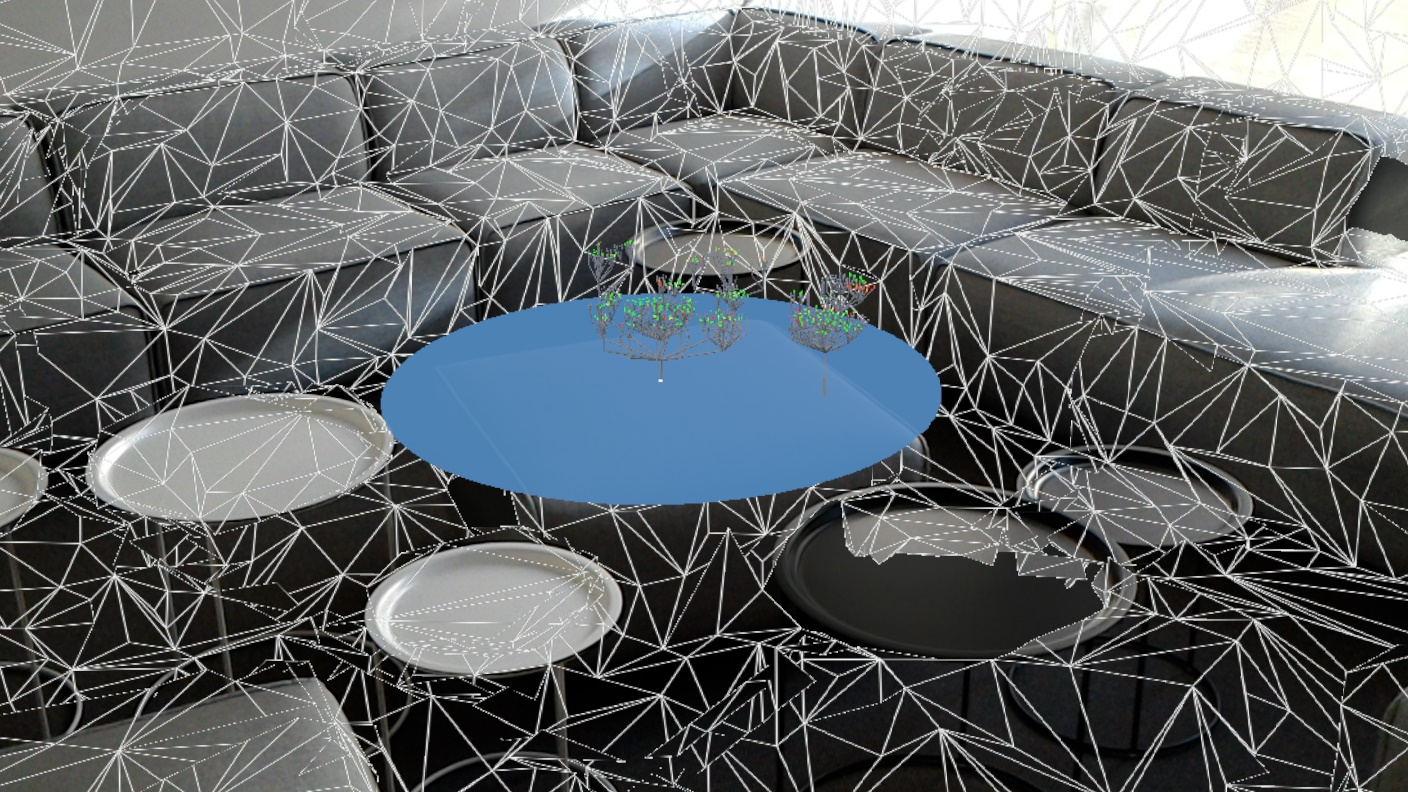
\includegraphics[width=.8\textwidth]{\figdir/spatial-mapping}
  \caption{Spatial Mapping beim Platzieren des Waldes}
  \label{fig:spatial-mapping}
\end{figure}

\section{Das Kontextmenü}
Das Kontextmenü, mit dem die verschiedenen Interaktionsmodi für den gesamten Wald ausgewählt werden können, lässt sich aber nicht nur für die Interaktion mit dem Waldboden anwenden. Auch für andere fokussierte Objekte ist eine vom Kontext abhängige Auswahl von möglichen Funktionen allgemeingültig sinnvoll. In herkömmlichen 2D Benutzeroberflächen ist dies mit einem Rechtsklick zu vergleichen. In 3D kann um den Punkt, den der Nutzer beim Aufruf des Kontextmenüs fokussiert hatte, das Kontextmenü in Form von Buttons in einer kreissegmentförmigen Anordnung dargestellt werden.

Die kreissegmentförmige Anordnung der Buttons hat den Vorteil, dass der Interaktionspunkt für das öffnen des Kontextmenüs im Zentrum des Kreises ist und daher eine Verbindung mit dem fokussieren Objekt schafft. Darüber hinaus sind alle Buttons vom Cursor gleich weit entfernt und daher schnellstmöglich mithilfe der Blickrichtung erreichbar.

Die Distanz des Kontextmenüs ist den Umständen entsprechend anzupassen. Ist der fokussierte Punkt bereits näher als die Distanz, in der eine Darstellung von Interaktions-Elementen empfohlen wird\footnote{Die Distanz, in der Microsoft empfiehlt Hologramme zu platzieren, liegt bei 2,0 Metern \cite{windows2017interaction}.}, sollte das Kontextmenü nicht noch näher an dem Nutzer platziert werden. Bei größerem Abstand sollte der Abstand zum Kontextmenü auf die empfohlene Distanz reduziert werden, sodass der Nutzer noch komfortabel mit dem Menü interagieren kann. Auf diese Weise ist die Überdeckung des Kontextmenüs durch andere Elemente sehr unwahrscheinlich.

In dem Fall, dass das Kontextmenü direkt an der fokussierten Position erscheint, muss das Kreissegment des Kontextmenüs so angepasst werden, dass die Buttons nicht in das fokussierte Objekt hinein ragen. Für den Waldboden ist daher ein nach oben orientiertes Kreissegment eine gute Wahl. Würde aber zum Beispiel mit einer Wand interagiert werden, sollte das Kontextmenü von der Wand weg orientiert sein.

Das Kontextmenü für den Waldboden im High-Fi Prototypen ist in Abbildung \ref{fig:context-menu} zu sehen. Mit dem vierten Button von links ist das App-Menü aufrufbar, dass in \ref{sec:app-menu} vorgestellt wird. 

\begin{figure}[htb]
  \centering
  \begin{subfigure}[b]{\fwidth}
    \centering
    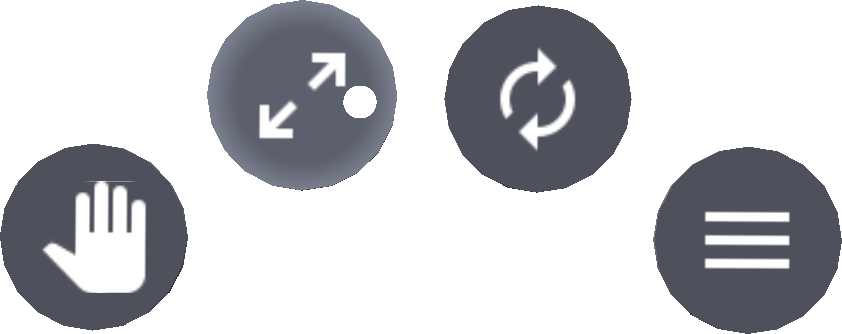
\includegraphics[height=2.5cm]{figures/context-menu-front}
    \subcaption{Kontextmenü aus Sicht des Nutzers} \label{fig:context-menu-front}
  \end{subfigure}
  \begin{subfigure}[b]{\fwidth}
    \centering
  	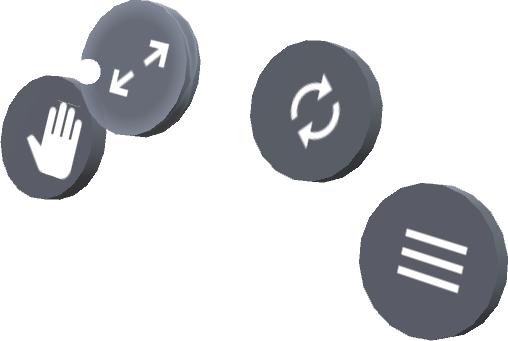
\includegraphics[height=2.5cm]{figures/context-menu-side}
  	\subcaption{Kontextmenü von der Seite} \label{fig:context-menu-side}
  \end{subfigure}
  \caption{Kontextmenü für den Waldboden im High-Fi Prototyp} \label{fig:context-menu}
\end{figure}

In Abbildung \ref{fig:context-menu-side} ist zu erkennen, dass der fokussierte Button räumlich hervorgehoben ist. Dies ist eine vor der AR noch nicht dagewesene Möglichkeit dem Nutzer haptisches Feedback zu geben. Angenommen $\vv{g}$ ist der Normalvektor der Blickrichtung des Nutzers, dann wird ein Button beim Fokussieren um $-\vv{g} \cdot x$ transformiert, wobei $x$ ein beliebiger Faktor ist. Bei der Ausführung der Air-Tap-Geste wird beim Schließen der Finger der Button um $\vv{g} \cdot x$ transformiert, sodass er wieder in seine Ausgangsposition gelangt. Sobald der Nutzer mit dem Öffnen der Finger den Air-Tap beendet, wird der Button wieder um $-\vv{g} \cdot x$ transformiert. Verlässt der Fokus den Button, wird er ebenfalls wieder in seine Ausgangsposition versetzt.

Mit diesem Prinzip wird einem Button ein haptisches Feedback verliehen und der Nutzer kann ihn räumlich "`eindrücken"'. Das Prinzip findet auch beim Windows-Menü der HoloLens Anwendung und zieht sich durch die gesamte UI des High-Fi Prototypen.

\section{Manipulation-Indicators}
\label{subsec:manipulation-indicators}
Mit dem Kontext-Menü des Waldbodens kann zwischen den beiden Interaktionsmodi umgeschalten werden, die mit der Manipulation-Geste ausgeführt werden. Bei der Manipulation-Geste weiß der Nutzer aber ohne weiter Hilfe nicht, wie er seine Hand bewegen muss, um die gewünschte Manipulation zu erreichen. Der Nutzer weiß nicht in welche Richtung der Wald vergrößert und in welche er verkleinert wird. Zudem sind mehrere Bewegungsachsen wie horizontal, vertikal oder diagonal denkbar. Deswegen ist es unerlässlich dem Nutzer Feedback zu geben. Dies wird mit den -- wie wir sie nennen -- \textit{Manipulation-Indicators} erreicht. Diese tauchen auf, sobald der Air-Tap gehalten wird und indizieren die möglichen Richtungen und deren Auswirkungen.

In Abbildung \ref{fig:manipulation} sind Manipulation-Indicators für das Beispiel des Skalierens dargestellt.

\begin{figure}[htb]
  \centering
  \begin{subfigure}[t]{\fwidth}
    \centering
    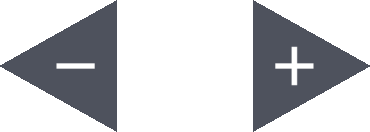
\includegraphics[height=1.5cm]{figures/manipulation}
    \subcaption{Initialer Zustand} \label{fig:manipulation}
  \end{subfigure}
  \begin{subfigure}[t]{\fwidth}
    \centering
  	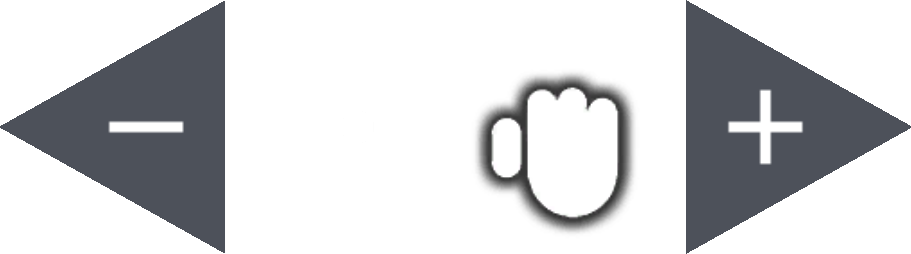
\includegraphics[height=1.5cm]{figures/manipulation-drag}
  	\subcaption{Darstellung des Deltas durch Bewegung der Pfeile} \label{fig:manipulation-drag}
  \end{subfigure}
  \caption{Manipulation-Indicators am Beispiel des Interaktions-Modus Skalieren} \label{fig:manipulation}
\end{figure}

Durch die Pfeile wird die Achse der Manipulation angegeben. In unserem Beispiel wird die Horizontale für die Skalierung verwendet. Durch die Symbole wird dem Nutzer eindeutig angezeigt, welche Richtung welche Auswirkung hat. Durch die Verschiebung der Pfeile um das Delta der Handposition, wird dem Nutzer zudem das Ausmaß seiner Eingabe widergespiegelt.

\section{Das App-Menü}
\label{sec:app-menu}

Bisher wurden Interaktionen behandelt, die nur bei einem vorhanden Wald relevant sind. Der Nutzer von CodeLeaves muss jedoch zuvor auswählen können, welche Software er überhaupt visualisieren möchte (Akz. \ref{acc:u-project-selection}). Auch müssen die dargestellten Informationen nach der Auswahl eines Projekts konfiguriert werden können (Akz. \ref{acc:s-metrics}, \ref{acc:s-thickness}, \ref{acc:d-metrics} und \ref{d-thickness}). Dafür wird ein zentrales \textit{App-Menü} eingeführt.

Für dieses Menü wurde sich an herkömmlichen Fenstern orientiert, wie sie bei Desktop-Systemen zu finden sind. Bevor näher auf den Inhalt des App-Menüs eingegangen wird, muss zunächst auf die Positionierung des Fensters im Raum eingegangen werden.

\subsubsection*{Positionierung}

Initial dient das App-Menü dazu ein Projekt auszuwählen bzw.\ eines von einer unterstützen Datenquelle zu importieren. Deshalb sollte das Menü nach dem Start der App in jedem Fall im Fokus des Nutzers platzieret werden, sodass dieser sofort mit CodeLeaves arbeiten kann. Dies kann mit dem in Abschnitt \ref{sec:interaction-hololens} vorgestellten Tag-along-Effekt bewerkstelligt werden. Für den initialen Zustand ist der Tag-along-Effekt des App-Menüs als nicht störend zu bewerten, da der Nutzer in jedem Fall mit dem Menü interagieren möchte und noch keine andren Inhalte vorhanden sind, die das Menü verdecken würde.

Nach der Auswahl eines Projekts kann der Tag-along-Effekt aber durchaus als störend empfunden werden, da er das Menü im Vordergrund hält und die Sicht auf den Wald versperrt. Das Fenster des App-Menüs muss demnach die Möglichkeit unterstützen stationär im Raum platziert oder ganz geschlossen zu werden.

Zweiteres kann mit einem Schließen-Button in einer Titelleiste realisiert werden, was dem Nutzer aus bekannten Systemen vertraut ist. Das erneute Öffnen kann und muss durch das Kontextmenü von Objekten des Waldes möglich sein. In Abbildung \ref{fig:context-menu} ist diese Möglichkeit im Kontextmenü des Waldbodens bereits zu sehen gewesen. Auch im Kontextmenü eines Blattes oder eines inneren Knotens sollte das App-Menü aufrufbar sein, da der Nutzer damit Eigenschaften der Blätter und inneren Knoten verändern kann.

Die Funktion des stationären Platzierens kann ebenfalls in der Titelleiste untergebracht werden. Analog zum "`Vollbild"' eines Desktop-Fensters, bei dem der Nutzer sich ausschließlich auf dieses konzentrieren möchte, wird neben dem Schließen-Button ein \textit{Tag-along-Button} eingeführt, der für das Ein- und Ausschalten des Tag-along-Effekts zuständig ist. Damit kann der Nutzer das Fenster jederzeit dort platzieren, wo es sich gerade befindet. Wird das App-Menü aus einem Kontextmenü aufgerufen, wird der Tag-along-Effekt aktiviert, sodass der Nutzer das Fenster nicht suchen muss, sondern es zu ihm kommt, sobald er es braucht.

Die Titelleiste kann für eine weitere Funktion genutzt werden. Wird bei Desktop-Systemen ein Drag-and-drop der Titelleiste durchgeführt, lässt das zugehörige Fenster verschieben. Dies ist in 3D ebenfalls möglich. Wird die Manipulation-Geste bei fokussierter Titelleiste durchgeführt, wird das Fenster des App-Menüs entsprechen im Raum verschoben. Durch die dreidimensionale Eingabe der Manipulation-Geste, kann der Drag-and-drop im Zweidimensionalen einfach in drei Dimensionen übertragen werden.

In dem High-Fi Prototyp wurden die beschriebenen Funktionen des App-Menüs bereits umgesetzt. In Abbildung \ref{fig:app-menu} kann das erstellte Menü betrachtet werden. Die Auswahl eines Projekts beschränkt sich dabei auf gespeicherte Beispielprojekte (Akz. \ref{acc:u-project-selection}).

\subsubsection*{Projektauswahl}

Für die produktive Einsetzung von CodeLeaves ist ein Import von neuen Projekten nötig (Akz. \ref{acc:u-import}). In dem Low-Fi Papier Prototyp in Abbildung \ref{fig:project-selection-mockup} ist die Interaktion mit zusätzlicher Import-Möglichkeit dargestellt.

\begin{figure}[htb]
  \centering
  \begin{subfigure}[t]{\textwidth}
    \centering
    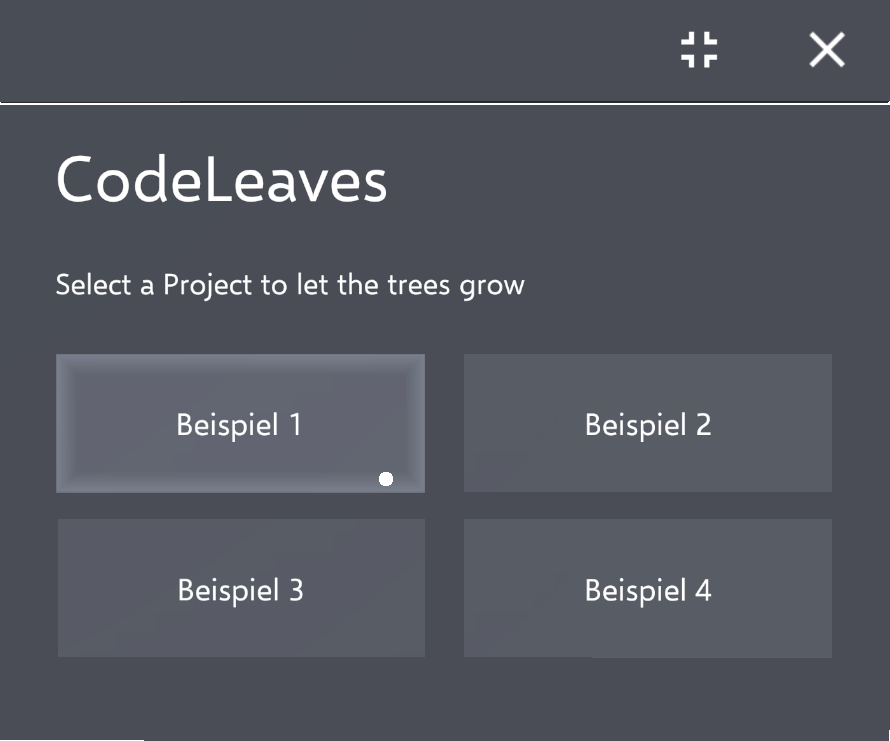
\includegraphics[width=.8\textwidth]{figures/project-selection}
    \subcaption{Initialzustand zur Auswahl eines Beispielprojektes und aktivem Tag-along} \label{fig:project-selection}
  \end{subfigure}
  \par\bigskip
  \begin{subfigure}[t]{\textwidth}
    \centering
  	
\includegraphics[width=.8\textwidth]{figures/title-bar}
  	\subcaption{Titelleiste mit deaktiviertem Tag-along} \label{fig:title-bar}
  \end{subfigure}
  \caption{High-Fi Prototyp der Projektauswahl im App-Menüs} \label{fig:app-menu}
\end{figure}

%Bei den hier vorgestellten Low-Fi Prototyp Darstellungen besteht kein Anspruch auf Vollständigkeit. Vielmehr müsste der Low-Fi Prototyp eine Evaluations-Phase mit Probanden durchlaufen, um diesen zu Bewerten und bei Bedarf zu überarbeiten. Auf diese Phase wird im Rahmen dieser Arbeit jedoch verzichtet, da es vor allem um das Design neuer Konzepte in der AR und das Grobkonzept gehen soll.

Bei der Projektauswahl hat der Nutzer die Wahl zwischen zwei Haupt-Tasks: Der Auswahl eines bereits betrachteten Projektes und dem Import von neuen Projekten. Die Interaktion bei einem Import ist für SonarQube beispielhaft im Anhang zu finden.

\begin{figure}[htb]
  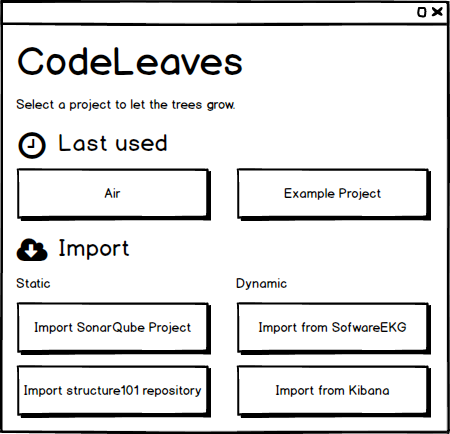
\includegraphics[width=.8\textwidth]{\figdir/project-selection-mockup}
  \caption{Low-Fi Prototyp der Projektauswahl im App-Menü}
  \label{fig:project-selection-mockup}
\end{figure}

Ist ein Projekt ausgewählt bzw.\ importiert, wird der Wald nach dem Layout generiert, das in Kapitel \ref{ch:layout} erarbeitet wurde. Danach wird dem Nutzer die Möglichkeit geboten, den Wald so anzupassen, dass er genau die Informationen zeigt, die der Nutzer sucht.

\subsubsection*{Einstellungen}

Dies kann er ebenfalls mit dem App-Menu erreichen, das sich nun in eine Schaltzentrale mit allen nötigen Einstellungen verwandelt. Im High-Fi Prototyp wurden nur essentielle Eistellungen eingebaut, die für die Nutzung des Prototyps unerlässlich sind. In Abbildung \ref{fig:settings} ist dagegen wiederum eine vollständige Low-Fi Prototyp Zeichnung zu sehen.

\begin{figure}[htb]
  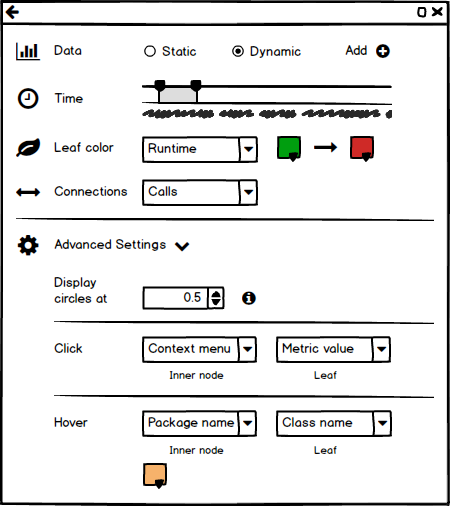
\includegraphics[width=.9\textwidth]{\figdir/app-menu-mockup}
  \caption{Low-Fi Prototyp für die Einstellungen im App-Menü}
  \label{fig:settings}
\end{figure}

Der Nutzer muss eine Metrik für die Farbe der Blätter (Akz. \ref{acc:s-metrics} und \ref{acc:d-metrics}) und ein Verbindungs-Typ für die Dicke der Wurzeln und Kanten (Akz. \ref{acc:s-thickness},  und \ref{d-thickness}) angeben können. Die Zuordnung von Metriken für die Farbe der Blätter und die Stärke der Verbindungen nehmen deshalb als Drop-down-Menüs zentrale Elemente in den Einstellungen ein.

Die zur Auswahl stehenden Metriken sind davon abhängig, ob der Nutzer gerade dynamische oder statische Daten betrachten möchte.

Deshalb wird als erstes die Wahl angeboten, ob statische oder dynamische Informationen betrachtet werden sollen. Mit dem "`Add"' neben dieser Auswahl kann der Nutzer Daten zu dem geladenen Projekt hinzufügen (Akz. \ref{acc:u-add-data}). Je nachdem welche Auswahl getroffen wird, kann der Nutzer darunter entweder einen Zeitpunkt -- in diesem Fall wird nur \textbf{ein} Schieberegler angezeigt -- oder einen Zeitraum angeben (Akz \ref{acc:s-timestamp} und \ref{acc:d-timespan}).

Die Drop-down-Menüs für die dargestellten Metriken passen sich ebenfalls der Auswahl von "`Data"' an. Damit sind die wichtigsten Einstellungsmöglichkeiten schon abgedeckt und der Nutzer kann die aktuell dargestellten Daten interaktiv erforschen.

D.\ Norman stellt im Interaction Design Klassiker \textit{The Design of Everyday Things} sieben allgemeingültige Prinzipien für gutes Interaction Design auf. Nach dem siebten Prinzip \textit{Constraints} sollten die möglichen Aktionen des Nutzers eigeschränkt werden, um die Aktionen zu lenken und den Nutzer nicht zu überfordern \cite{norman2013design}. Dies lässt sich auch auf die Einstellungen für CodeLeaves anwenden.

Mit den bisher beschriebenen Einstellungen ist der Nutzer bereits in der Lage den Wald als Ganzes zu konfigurieren. Weitere optionale Einstellungen werden deswegen in "`Advanced Settings"' gekapselt, sodass sich der Nutzer damit nicht auseinandersetzten muss, wenn er das nicht möchte. Der fortgeschrittene Nutzer findet dort jedoch nützliche Anpassungen.

Zum einen hat er die Möglichkeit den verfügbaren Eingabemöglichkeiten eine Aktion zuzuweisen (mehr dazu in Abschnitt \ref{sec:object-interaction}).

Zum anderen ist in den "`Advanced Settings"' die Einstellung "`Display circles at"' zu finden, die durch das Prototyping des High-Fi Prototyp entstanden ist.

\subsubsection*{Umschließende Kreise zur erleichterten Bedienung}
Die Kreise, die zur Visualisierung des Circle-Packings im Abbildung \ref{fig:Circle-Packing} dargestellt sind, haben sich auch für die Interaktion als überaus hilfreich erwiesen. CodeLeaves hat auf der HoloLens mit folgendem Problem umzugehen:

\begin{quote}
  \textit{Je kleiner der Wald skaliert wird, desto schwieriger wird die Interaktion mit einzelnen Blättern oder Kanten.}
\end{quote}

Abhilfe schaffen die umschließenden Kreise, die als Ziel der Interaktion dienen können. Ein Knoten besitzt bei aktivierten Kreisen als Alternative zur Kante für die Interaktion auch seinen Kreis, der deutlich mehr Fläche für die Interaktion bietet.

Abbildung \ref{fig:circle-hover} zeigt die Interaktion mit einem Kreis am Beispiel der Fokussierung. Auf diese Aktion wird im nächsten Abschnitt eingegangen.
 
\begin{figure}[htb]
  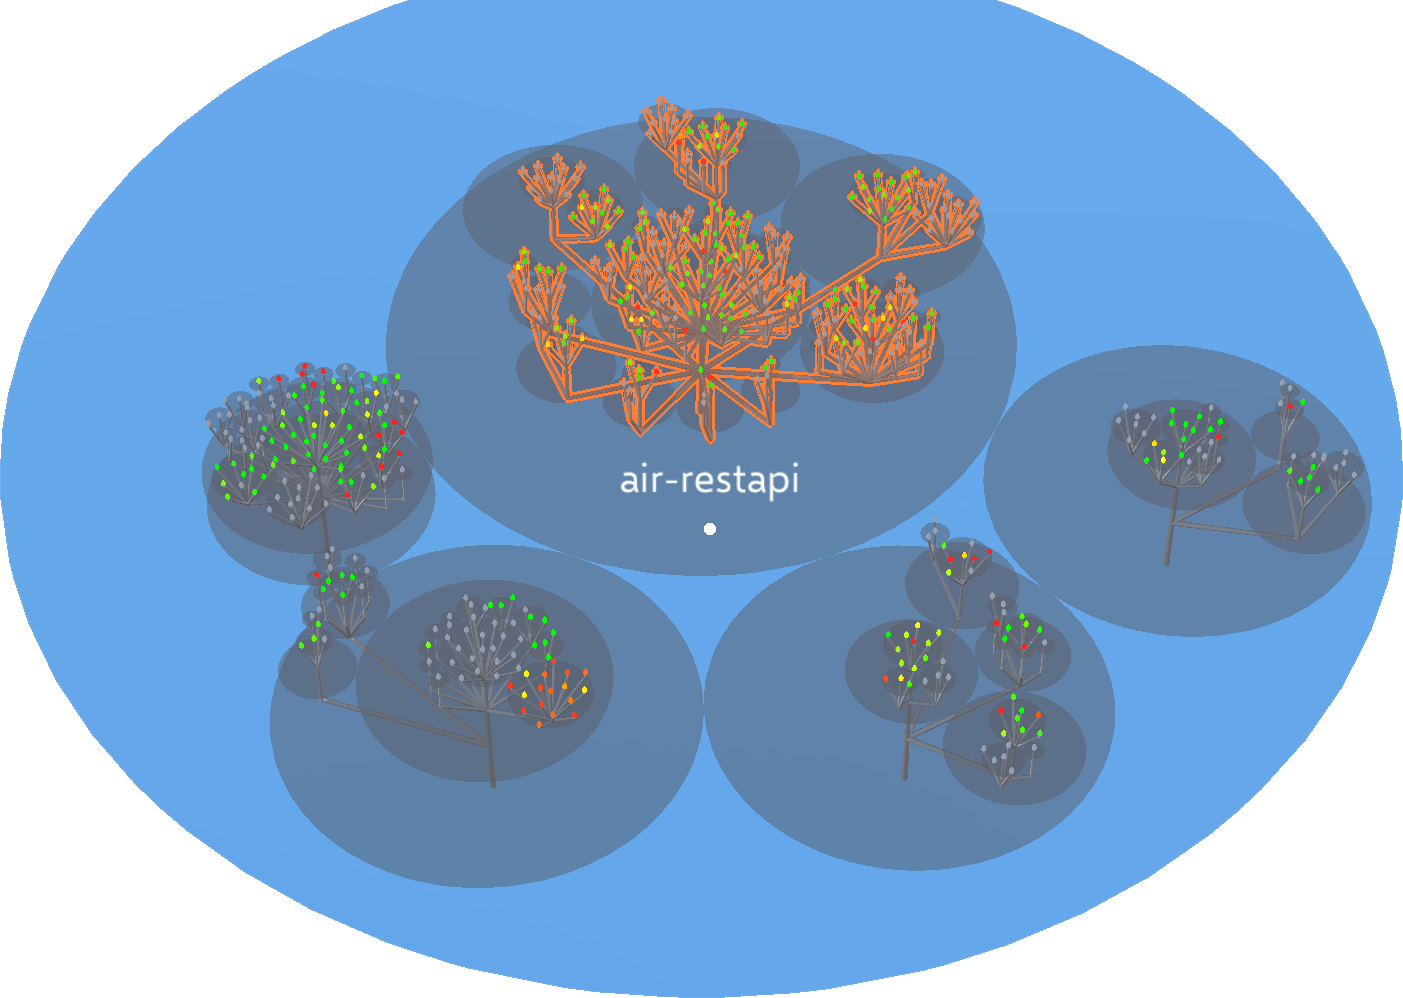
\includegraphics[width=.8\textwidth]{figures/circle-hover}
  \caption{Visualisierung der Kreise für leichtere Interaktion}
  \label{fig:circle-hover}
\end{figure}

Durch die Einstellung für die Kreise ist konfigurierbar ab welchem Skalierungsfaktor des Waldes die Kreise angezeigt werden. Standardmäßig würde dies der Fall sein, sobald die Interaktion mit einzelnen Blättern oder Kanten nicht mehr komfortabel möglich ist. Der Schwellenwert dafür müsste durch weiterführende Nutzer-Befragungen evaluiert werden.

\section{Interaktion mit Blättern, inneren Knoten und Wurzeln}
\label{sec:object-interaction}

Mit dem App-Menü haben wir die Möglichkeit die Daten auszuwählen, die der Wald darstellt. Was noch fehlt ist die direkte Interaktion mit den Objekten des Waldes -- mit den Blättern, inneren Knoten und Wurzeln. Mit der Blickrichtung und den verfügbaren diskreten Gesten der HoloLens, gibt es insgesamt vier verschiedene Eingabemöglichkeiten, mit denen der Nutzer mit den Objekten in Interaktion treten kann:

\begin{itemize}
  \item Fokus
  \item Tap (Air-Tap)
  \item Double-Tap
  \item Tap-and-hold
\end{itemize}

Da es aber für jedes Objekt mehr mögliche Aktionen als Eingabemöglichkeiten gibt, ist das Kontextmenü immer durch mindestens eine Eingabemöglichkeit erreichbar und bietet alle verfügbaren Aktionen an.

Bevor wir eine Übersicht aller Aktionen und deren mögliche Zuordnung betrachten, widmen wir uns zunächst dem Fokus.

\subsubsection*{Fokus}

A. Cooper ist in \cite{cooper2014face} der Meinung, dass ``constant [...] feedback is exactly what users need''. So sollte abgesehen von weiteren Auswirkungen dem Nutzer immer Feedback zum aktuellen Fokus gegeben werden. Der Nutzer muss zu jeder Zeit wissen, welches Objekt er gerade fokussiert, was dazu gehört und dass er damit interagieren kann. In CodeLeaves wird dies bei Objekten des Waldes durch einen farbigen Umriss erreicht. Bei inneren Knoten werden auch alle Nachfahren hervorgehoben, da auf fachlicher Ebene alle Unterpakete auch Teil eines Pakets sind. So ist zum Beispiel auch immer zu erkennen welche Äste zu welchem Baum gehören, auch wenn die Bäume hintereinander stehen.

Wird die Hervorhebung aber sofort aktiv, sobald die Blickrichtung ein Objekt trifft, hat das zur Folge, dass beim "`Blick schweifen lassen"' die Objekte nur kurz aufflackern. Bei der Entwicklung des High-Fi Prototyps konnte festgestellt werden, dass diese Art der Hervorhebung zu schnell und unangenehm ist.

Um das zu vermeiden, wird das Feedback des Fokus verzögert, sodass es erst sichtbar wird, sobald der Fokus einen bestimmten Zeitraum auf demselben Objekt verweilt. Ein passendes Pendant bei Desktop-Anwendungen wären Tooltips, die erst angezeigt werden, wenn der Mauszeiger über einem Element verweilt.

Für den festzulegenden Zeitraum wurde sich an den Arbeiten \cite{miller1956magical} und \cite{mishunov2015why} orientiert. Dort ist von der sogenannten \textit{Immediate Behaviour} die Rede, die in einem Zeitraum von 0,5 bis 1 Sekunde statt finden sollte. Dieser Zeitraum ist die Zeit, die ein Gesprächspartner gewöhnlich benötigt, um in einer Mensch-zu-Mensch Kommunikation zu antworten und die auch in Mensch-zu-Maschine Kommunikation eingehalten werden sollte.

Mit dieser Lösung ist es möglich sich im Wald in Ruhe umzuschauen und sobald der Fokus länger auf einem Objekt bleibt, wird das Objekt hervorgehoben. So weiß der Nutzer zu jeder Zeit mit welchem Objekt er gerade interagiert.

\subsubsection*{Übersicht über mögliche Aktionen}

In der Tabelle \ref{tab:actions} können alle verfügbaren Aktionen betrachtet werden. Die Icons in der zweiten Spalte befinden sich zur Wiedererkennung zum Teil auch in den Abbildungen des Low-Fi Prototypen der Kontextmenüs. In den letzten drei Spalten ist zu finden mit welcher Eingabe die Aktion für welches Objekt aufrufbar ist. Ist eine Zelle darin leer, ist die Aktion für das entsprechende Objekt nicht möglich. "`KM"' steht dafür, dass die Aktion über das Kontextmenü aufrufbar ist.

\renewcommand\tabularxcolumn[1]{m{#1}}
\newcommand{\icon}[1]{\vspace{-8px}\includegraphics[width=24px]{figures/icons/#1}}
\begin{tabularx}{\textwidth}{lm{1cm}L*{3}{C{2cm}}}
  \caption{Mögliche Aktionen und deren Erreichbarkeit}\label{tab:actions} \\
  \tableheader{6}{\textbf{ID} & \multicolumn{2}{l}{\textbf{Aktion}} & \textbf{Blatt} & \textbf{innerer Knoten} & \textbf{Wurzel}}
   1 & \icon{info} & Name der Klasse, des Pakets bzw.\
           der verbundenen Pakete anzeigen (Akz. \ref{acc:u-identify})& Fokus        & Fokus         & Fokus        \\
   2 & \icon{context-menu} & Kontextmenü aufrufen                     & Tap-and-hold & Tap-and-hold  & Tap-and-hold \\
   3 & \icon{metric} & Wert der aktuellen Metrik anzeigen
        (Akz. \ref{acc:s-metric-value} und \ref{acc:s-metric-value})  & Tap          &               &              \\
   4 & \icon{list} & Liste mit allen Metriken anzeigen                & KM           &               &              \\
   5 & \icon{direction-count} & Anzeigen wie vielen Verbindungen
        in welche Richtung gehen (Akz. \ref{acc:s-connection-count}
        und \ref{acc:d-connection-count})                             &              & Tap           & Tap          \\
   6 & \icon{connections} & Zugeordnete Verbindungen hervorheben
        (Akz. \ref{acc:s-leaf-connections},
        \ref{acc:d-leaf-connections},
        \ref{acc:s-connection-highlight} und
        \ref{acc:d-connection-highlight})                             & Double-Tap   & Double-Tap    & Double-Tap   \\
   7 & \icon{connections-in} & Eingehende Verbindungen hervorheben    & KM           & KM            &              \\
   8 & \icon{connections-out} & Ausgehende Verbindungen hervorheben   & KM           & KM            &              \\
   9 & \icon{right} & Verbindungen nach Rechts hervorheben            &              &               & KM           \\
  10 & \icon{left} & Verbindungen nach Links hervorheben              &              &               & KM           \\
  11 & \icon{web} & Verbindungen direkt anzeigen                      & KM           & KM            &              \\
  12 & \icon{mark} & Objekt zum späteren Wiederfinden markieren       & KM           & KM            & KM           \\
  13 & \icon{full-screen} & Wald so skalieren, dass die Auswahl das
           ganze Sichtfeld der HoloLens einnimmt                      &              & KM            &              \\
  13 & \icon{as-floor} & Knoten als neuen Waldboden verwenden
       (Akz. \ref{acc:s-drilldown})                                   &              & KM            &              \\
\end{tabularx}

Die Zuordnung der Aktionen zu den vorhanden Eingabemöglichkeiten kann, wie in Abschnitt \ref{sec:app-menu}, Abbildung \ref{fig:settings} zu sehen, bei Bedarf vom Nutzer angepasst werden. Dies ist sinnvoll, wenn der Nutzer mit einer anderen Zuweisung schneller oder komfortabler an gesuchte Informationen gelangt. Möchte der Nutzer zum Beispiel nur Klassen mit niedriger Testabdeckung identifizieren, ist es sinnvoll wie in Tabelle \ref{tab:actions} angegeben bei einem Air-Tap auf ein Blatt den Wert der Testabdeckung anzuzeigen. Ist der Nutzer jedoch ausschließlich an statischen Abhängigkeiten interessiert, kann er anstatt den standardmäßigen Double-Tap auch einen einfachen Air-Tap für die Anzeige der zugehörigen Verbindungen verwenden.

Im Folgenden werden einige Aktionen noch genauer beschrieben. \\

\newcommand{\inlineicon}[1]{
  \setlength\intextsep{0pt}
  \begin{wrapfigure}[2]{l}{24px}
    \vspace{-2px}
    \includegraphics[width=24px]{figures/icons/#1}
  \end{wrapfigure}
}

\begingroup

\inlineicon{info}\noindent Die Anzeige der Namen von Klassen und Paketen ist für deren Identifikation besonders wichtig, da der Nutzer nur so weiß, welchen Teil der Software er vor sich sieht. Der Fokus ist dafür komfortabel, da ein fokussiertes Objekt zwangsläufig immer das ist, wofür sich der Nutzer interessiert und der Nutzer nicht dauerhaft Air-Taps durchführen muss, um sich umzuschauen. Der angezeigte Name befindet sich aus Nutzersicht immer über dem Cursor und wird dem Abstand entsprechend so skaliert, dass der Text immer gleich groß erscheint. Wichtig ist dass der Text in der Entfernung des fokussierten Objekts angezeigt wird, und nicht etwa wie das Kontextmenü innerhalb von zwei Metern, da der Nutzer sonst immer zwischen unterschiedlichen Raumtiefen hin- und herschauen muss.\\

\inlineicon{context-menu}\noindent Das Kontextmenü ist für jedes Objekt aufrufbar, da nur so alle Aktionen erreichbar sind. Die Tap-and-hold-Geste eignet sich für das Kontextmenü, da diese Eingabe bei touchbasierten Eingabegeräten ebenfalls oft für Kontextmenüs verwendet wird.\\

\inlineicon{metric}\noindent Beim Blatt kann der genaue Wert einer Metrik durch einen einfachen Air-Tap aufgerufen werden. Durch die Liste aller Metriken, die der Nutzer über das Kontextmenü aufrufen kann, kann der Nutzer eine bestimmte Klasse genauer untersuchen, ohne die aktuelle Metrik umstellen zu müssen.\\

\inlineicon{direction-count}\noindent Mit der Anzahl der Verbindungen ist ersichtlich wie die Dicke der Verbindung zustande kommt.\\

\inlineicon{connections}\noindent Durch das Hervorheben der Verbindungen kann der Nutzer sehen, zu welchen Blättern die Verbindungen gehören. Die Anzahl der Verbindungen können dabei ebenfalls angezeigt werden. Dieser Fall ist am Beispiel einer Wurzel in Abbildung \ref{fig:root-interaction} illustriert. Führt der Nutzer ein Air-Tap auf eine Kante mit bereits hervorgehobener Verbindung aus, werden nur die Verbindungen hervorgehoben, die in der vorherigen Auswahl enthalten waren und die durch die ausgewählte Kante fließen. Mit diesem Prinzip kann jede Verbindung immer feiner Untersucht werden.\\

\begin{figure}[htb]
  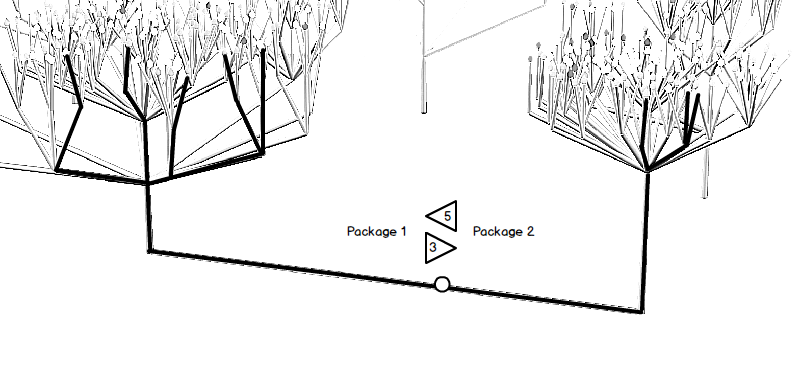
\includegraphics[width=\textwidth]{figures/root-interaction}
  \caption{Hervorhebung und Anzeige der Anzahl und Richtung von einzelnen Verbindungen einer Wurzel}
  \label{fig:root-interaction}
\end{figure}

\inlineicon{connections-in}\noindent Mit den Aktionen 7 - 10 ist es möglich eine Vorauswahl der hervorgehobenen Verbindungen zu treffen. Zum Beispiel würden im Szenario aus Abbildung \ref{fig:root-interaction} mit Aktion 9 nur die 3 Verbindungen gezeigt, die von Package 1 nach Package 2 fließen. Der Aufruf dieser Aktionen ist nicht nur im Kontextmenü, sondern auch durch den Air-Tap auf die Pfeile für die Richtungsangaben möglich. \\

\inlineicon{web}\noindent Jedes Objekt hat im Kontextmenü die Option die gerade ausgewählten Verbindungen auch direkt als Spinnweben anzuzeigen.\\

\inlineicon{mark}\noindent Aktion 12 ist komfortabel, wenn Interesse an bestimmten Klassen besteht und vielleicht unterschiedliche Daten und Metriken hintereinander ausgewählt werden und der Nutzer ein Objekt schnell wieder finden möchte.\\

\inlineicon{full-screen}\noindent Die Möglichkeit ein Paket so zu vergrößern oder zu verkleinern, dass es genau in das Sichtfeld der HoloLens passt, ist bei dem kleinen Sichtfeld der HoloLens eine Funktion, die die User-Experience durchaus positiv beeinflussen und den Workflow beschleunigen kann.\\

\endgroup

Abschließend zu Interaktion mit Blättern, Kanten und Wurzeln, ist in \ref{fig:leaf-contextmenu} das Kontextmenü für  Blätter dargestellt. Auf der rechten Seit (\ref{fig:leaf-contextmenu-connections}) sehen wir eine Unterauswahl, die aufgeht, sobald der Nutzer auf das Symbol der Verbindungen tippt. Auf diese Weise sind auch gruppierte Kontextmenüs möglich.

Die Kontextmenüs für Kanten und Wurzeln sind im Anhang zu finden.

\begin{figure}[htb]
  \centering
  \begin{subfigure}[b]{\fwidth}
    \centering
    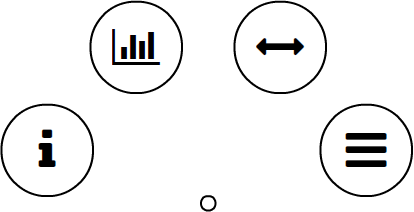
\includegraphics[scale=0.45]{figures/leaf-contextmenu}
    \subcaption{Initialer Zustand} \label{fig:leaf-contextmenu-initial}
  \end{subfigure}
  \hfill
  \begin{subfigure}[b]{\fwidth}
    \centering
  	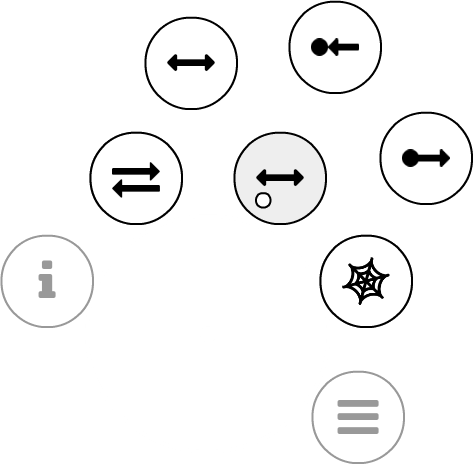
\includegraphics[scale=0.45]{figures/leaf-contextmenu-connections}
  	\subcaption{Unterauswahl für Verbindungen} \label{fig:leaf-contextmenu-connections}
  \end{subfigure}
  \caption{Kontextmenü für ein Blatt} \label{fig:leaf-contextmenu}
\end{figure}

\chapter{Zusammenfassung und Ausblick}
\label{ch:conclusion}

\section{Zusammenfassung}

Zu Beginn haben wir uns dem Thema AR genähert und evaluiert, wieso AR gut für 3D Softwarevisualisierung geeignet ist. Auf dieser Basis wurde im \ref{ch:concept}.\ Kapitel CodeLeaves vorgestellt, um das neue Konzept zu erfassen und dessen Stärken kennen zu lernen. Mit der Wald-Metapher können Software-Strukturen mit Bäumen hervorragend visualisiert werden. Die ausgewählte Software wird zum Wald, Pakete zu Bäumen und Ästen und Klassen werden zu Blättern. Ein Wurzelgeflecht verbindet einzelne Bäume.

Auf das Blätterdach lassen sich ausgezeichnet verschiedene Metriken anwenden. Mit einem sommerlichen Grün bis hin zu einem herbstlichen Rot verschafft der Wald mit einem Blick eine Übersicht über die gesamte Software. Besonders Bäume oder Äste mit rötlicher Laubfärbung stechen in einem sonst grünen Wald besonders gut hervor.

Nicht nur Metriken lassen sich mit CodeLeaves darstellen, auch Verbindungen zwischen einzelnen Klassen. Seien es statische Abhängigkeiten, oder dynamische Aufrufe -- CodeLeaves kann Verbindungen durch die vorhandenen Baumstrukturen aggregieren und so übersichtlich anzeigen. Was bei anderen Visualisierungen ein undurchdringliches Dickicht an Pfeilen ist, wird zur Dick der Kanten und Wurzeln. Je mehr aggregierte Verbindungen durch eine Kante oder Wurzel fließen, desto dicker wird sie. Durch diese Darstellung kann schon ohne jegliche Interaktion eine gute Übersicht über die Kopplung einer Software geschaffen werden.

Verbindungen können interaktiv ebenfalls direkt angezeigt werden und fügen sich als Spinnweben zwischen den Bäumen nahtlos in die Metapher des Waldes ein.

In Kapitel \ref{ch:data-model} wird ein Datenmodell entwickelt, das einerseits Schichtentrennung zwischen Backend, Business-logic und Presentation ermöglicht und andererseits die Visualisierung von statischen und dynamischen Daten ermöglichen. Diese Möglichkeit ist ein Alleinstellungsmerkmal von CodeLeaves.

Im Zuge dieser Arbeit wurde ein High-Fi Prototyp für die HoloLens entwickelt. Primäres Ziel dabei war es Algorithmen für die Generierung der 3D Baumstrukturen zu suchen und grundlegende Interaktionen zu implementieren.

Die verwendeten Algorithmen und die dafür nötige Mathematik wird in Kapitel \ref{ch:layout} beschrieben. Es wird gezeigt wie sich Verhalten in der Natur mit dem Goldenen Schnitt auf die Bäume von CodeLeaves übertragen lassen. Mit dem Sonnenblumen-Algorithmus werden Blätter eines Elternteils gleichmäßig auf einer Kreisfläche verteilt, sodass sie den gleichen Abstand zueinander haben.

Durch hierarchisches Circle-Packing werden die Knoten der Bäume so verteilt, dass Äste sich nicht überschneiden können und alle Blätter des Waldes von oben betrachtet sichtbar sind.

Im Zuge des High-Fi Prototypen wurde auch festgestellt, dass sich die HoloLens in der aktuellen Entwickler-Version nicht für die Betrachtung von sehr großen Software-Systemen eignet, da die Visualisierung sonst nicht mehr flüssig gerendert wird.

Neben dem Layout des Waldes wurde die Interaktion mit CodeLeaves intensiv behandelt. Dafür wurden in Kapitel \ref{ch:interaction-ar} Grundlagen erarbeitet. Die zur Verfügung stehenden Eingabemöglichkeiten der HoloLens wurden vorgestellt und allgemeine Herausforderungen der Interaktion in der AR beleuchtet. Mit reaktiver Programmierung wurde zudem praxisnah erläutert, wie Interaktionen in Unity sinnvoll umgesetzt werden können.

Zu guter Letzt wurden die im High-Fi Prototypen bereits umgesetzten Interaktionen in Kapitel \ref{ch:interaction} aufgegriffen und durch ein Low-Fi Prototypen ergänzt. Mit dem universellen Kontextmenü und den Manipulation-Indikators wurden Interaktions-Elemente eingeführt, die auch in anderen Anwendungen ausgezeichnet Verwendung finden können. Das erarbeitete Interaktions-Konzept ermöglicht es den Wald interaktiv bis ins Detail zu erkunden.

\section{Ausblick}

Mit dem High-Fi Prototyp wurden bereits die wichtigsten Schritte für eine einsatzfähige Softwarevisualisierung gegangen. Für den produktiven Einsatz sind jedoch noch einige Schritte zu gehen.

\paragraph{Datenanbindung} 

Der Import von Daten benötigt ein Interface, wie es in Abbildung \ref{fig:project-selection-mockup} und \ref{fig:sonarqube-import} skizziert ist. Neben SonarQube für die Struktur der Software und deren statischen Metriken gilt es weitere Import-Möglichkeiten anzubieten. Für statische Abhängigkeiten bietet sich \textit{strucute101}\footnote{Structure101 ist eine agile Architektur-Entwicklungs-Umgebung (ADE), mit der das Software-Entwicklungsteam eine Codebasis organisieren kann (aus dem Englischen aus \cite{headway2017structure101}).} an. Mit structure101 sind Abhängigkeiten auf Klassenebene verfügbar. Der Export der Daten von structure101 wurde bereits erfolgreich getestet und muss als nächsten Schritt in das Modell von CodeLeaves gebracht werden.

Für dynamische Daten lässt sich zum Beispiel das Software-EKG der QAware verwenden. Die EKG-Kollektoren sammeln dynamische Daten aus unterschiedlichen Datenquellen wie der Programmschnittstelle JMX und Windows Performance Counter \cite{weigend2011dynamische}. Das Software-EKG besitzt eine eigene UI zur Darstellung der gesammelten Daten. Statt dieser Visualisierung müssten die Daten in CodeLeaves importiert und auf die Struktur der Software übertragen werden.

\paragraph{Evaluation der Aggregation}

Liegen ausreichend Testdaten für Verbindungen in Form des Software-Meta-Modells vor, muss die Anzahl der Einzelverbindungen auf die Dicke der Kanten und Wurzeln übertragen werden. Die Erweiterung des Prototypen für Unterstützung dieser Funktionalität ist gering, da der Prototyp bereits unterschiedliche Dicken von Kanten und Wurzeln generieren kann. Jedoch muss diese Funktionalität mit realistischen Daten evaluiert werden.

\paragraph{Evaluierung des Interaktionskonzepts}

Das Interaktionskonzept, das im Rahmen dieser Arbeit erarbeitet wurde, muss mit Test-Nutzern evaluiert werden. In diesem Zuge kann das Konzept überprüft und bei Bedarf überarbeitet werden. Anschließend müssen die fehlenden Elemente wie die Kontextmenüs für Blätter, innere Knoten und Wurzeln ergänzt werden.\\

Mit dem Import von Daten, der Umsetzung der aggregierten Verbindungen und der vollständigen Umsetzung des evaluierten Interaktionskonzept ist CodeLeaves einsatzfähig. Mit der HoloLens sind darüber hinaus noch Erweiterungen möglich.

\paragraph*{Sprachsteuerung}

Durch die Sprachsteuerung, die in die HoloLens integriert ist, könnten einige Interaktionen eventuell noch komfortabler gestaltet werden. Die Arbeit mit dem Air-Tap kann für den Arm des Nutzers auf Dauer ermüdend sein. Die Sprachsteuerung kann daher für einige Interaktionen sinnvoll als Alternative zum Air-Tap genutzt werden. Auch zusätzliche Aktionen wie "`Zeige mir die Klasse \enquote*{ExampleClass}"' sind mit Sprachsteuerung möglich und besonders komfortabel.

\paragraph*{Nutzung für mehrere Nutzer}
Die Möglichkeit holographische Inhalte gleichzeitig mit anderen Nutzern teilen zu können, ist ein großer Vorteil der AR. Diese muss jedoch auch in HoloLens-Applikationen implementiert werden. Microsoft stellt dafür die \textit{HoloToolkit.Sharing}-Bibliothek zur Verfügung. Diese Bibliothek wurde ursprünglich für das Projekt \textit{OnSight} entwickelt, eine Zusammenarbeit zwischen einem Microsoft Studio und der NASA, um das Rover-Planungstool der NASA durch die Nutzung von HoloLens Geräten zu erweitern. Apps, die das Teilen unterstützen, laufen auf mehreren HoloLens Geräten gleichzeitig und kommunizieren und synchronisieren sich in Echtzeit, sodass Nutzer gemeinsam an einer Aufgabe arbeiten können \cite{microsoft2017sharing}.

Der Einbau der Möglichkeit den Wald gemeinsam zu erkunden, wäre eine überaus spannende weiterführende Aufgabe, die CodeLeaves noch attraktiver machen würde.\\


  